\documentclass[a4paper, 12pt, openany, oneside]{book} %chose the paper size and font size. Openany ensures that all all chapters and similar may begin at any page, not only odd pages. For the introductory pages and appendices we want openany, but for chapter pages in the main content we want chapters to begin only on odd pages (right hand side). The book class ensures that the margins are automatically adjusted such that left hand pages are slightly moved to the left and vice versa at the right, which makes the thesis very readable and good looking when printed in bound book format.
\usepackage[utf8]{inputenc} %to manage special characters
\usepackage[T1]{fontenc} %to manage special characters
\usepackage[Bjarne]{fncychap} %fancy chapter style (many more available, like Sonny or Lenny etc.)
\usepackage{fancyhdr} %to customize the headers
\usepackage[lmargin=1.5in, rmargin=1in, tmargin=1in, bmargin=1in]{geometry} %sets the margins for the pages
\setcounter{tocdepth}{2} %table of contents number depth for subsections (2 = x.x.x)
\setcounter{secnumdepth}{4} %numbering depth for headers for subsections in the text(4 = x.x.x.x)
\usepackage{url} %to include urls
\usepackage{listings} %include this if you want to include code in the thesis
\usepackage{amsmath,amssymb} %mathematical package
\usepackage{siunitx} %includes SI-units
\usepackage[bf]{caption} %makes float captions bold
\captionsetup[subfigure]{margin=8pt}
\usepackage{array, booktabs} %to make better tables
\usepackage{graphicx} %to include graphics
\usepackage{enumerate} %enumarte lists
\usepackage{float} %to include floats
\usepackage[export]{adjustbox} %to adjust floats
\usepackage{subfig} %to include subfigures
\usepackage{chngcntr} %will make it possible to change the counter for tables, figures etc. such as below
\counterwithout{figure}{section} %change counter for figures within sections (also possible to choose for each chapter
\counterwithout{table}{section} %change counter for tables within sections
\usepackage{color, xcolor} %edit e.g. text colors
\usepackage{hyperref}
\usepackage{cleveref}
\usepackage{appendix}
%\usepackage[backend = biber,
%            style = numeric,
%            date = long,     % Long: 24th Mar. 1997 | Short: 24/03/1997
%            sorting = none,
%            maxcitenames = 3,   % max names to include before et. al.
%            ]{biblatex} %customize the look of your citations and bibliography
\usepackage{natbib}
\bibliographystyle{agsm}
%\addbibresource{bibliography.bib} %declare the bibliography resource
\usepackage{comment} %to be able to comment out sections in the .tex files
\usepackage{afterpage} %to customize page commands such as below
\newcommand\myemptypage{
    \null
    \thispagestyle{empty}
    \addtocounter{page}{-1}
    \newpage
    } %sets new page command to insert an empty page without adding to the page counter or having a page number

\usepackage{listings}
\usepackage{color}
\usepackage{url}
    
\lstset{ 
    language=R,
    basicstyle=\ttfamily\small,
    commentstyle=\color{green},
    keywordstyle=\color{blue},
    numbers=left,
    numberstyle=\tiny\color{gray},
    stepnumber=1,
    numbersep=5pt,
    backgroundcolor=\color{white},
    showspaces=false,
    showstringspaces=false,
    showtabs=false,
    frame=single,
    captionpos=b,
    breaklines=true,
    breakatwhitespace=false,
    escapeinside={\%*}{*)},
}


\begin{document}
%%%%%%%%%%%%%%%%%%%%%%%%%%%%%%%%%%%%%%%%%%%%%%%%%%%%%%%%
%\begin{comment}
% The title page:
% For NTNU students this page will be generated automatically when submitting your paper, and should not be included in the final file from Latex. Delete or comment out the title page setup. The final report should then start with the first page being the abstract. I have included a title page here so it is possible to see how it may look like, and for those who does not get an automatically generated title page. Of course you will need to change the names and titles etc. to your case.

%the title page should be an odd page (right hand side)

\begin{titlepage}
\newgeometry{left=1.6in, right=2in}
\vspace*{1.5cm}

\noindent  \textcolor{gray}{\large August Arnstad} \\
\vspace{1cm}

\noindent \textbf{\Large Relative variable importance in Bayesian linear mixed models} \\
\vspace{0.5cm}

%\noindent {\large Any undertitle is written here} \\



\vspace{7cm}
\noindent TMA4500 Project thesis in Industrial Mathematics \\
Supervisor: Stefanie Muff \\
December 2023 \\

\vspace{0.2cm}
\noindent Norwegian University of Science and Technology \\
Faculty of Information Technology and Electrical Engineering \\
Department of Mathematical Sciences \\

\begin{figure}[h]
    
\includegraphics[width=0.28\textwidth]{Figures/ntnu_basic.png}
\end{figure}
\end{titlepage}
\restoregeometry
\myemptypage %empty page such that the abstract starts at the first right hand side after the title page
%\end{comment}
%%%%%%%%%%%%%%%%%%%%%%%%%%%%%%%%%%%%%%%%%%%%%%%%%%%%%%%%

% The pre-chapters
\chapter*{Abstract} %pre-chapters should not be numbered, hence the "*"
\pagenumbering{roman} %introductory pages should be roman
\setcounter{page}{1}
\addcontentsline{toc}{chapter}{\protect\numberline{}Abstract} %add the chapter to the table of contents, this is not automatically added when creating unnumbered chapters (*). Add it in a chapter style, and keep all chapters on the same numberline indent regardless of number or not on the chapter
Statistical inference about the parameters of a model is a fundamental part of statistical analysis. 
In many applications it is desirable to understand how important each covariate is in explaining the observed response variable.
By specifying the importance of each variable, researchers gain a better understanding of the complex relationships in the statistical model, thereby improving their knowledge and quality of research.
Currently, there are several methods that try to deduce the importance of variables in a statistical model.
These methods include testing a null hypothesis by using parameter estimates, confidence intervals or $p$-values
This thesis aims to provide a method that decomposes the model variance in a Bayesian framework, to emphasize statistical inference rather than threshold-based interpretations, for example regarding a covariate as significant if $p<0.05$.
\newline
\newline 
We introduce a Bayesian measure of variable importance, which we call the \textit{Bayesian Variable Importance} (BVI) method. 
The BVI method adapts the key aspects of established methods for decomposing the variance of a random intercept model, into the Bayesian framework.
To do this, we use the relative weights method as our starting point.
The relative weights method, which can be considered an approximation of more computationally exhausting methods, projects correlated covariates into an uncorrelated space.
In the respective space the Bayesian model is fit, and the results are back-transformed to the original covariate space. 
The results include posterior distributions for each model covariate and the calculated variance that each covariate contributes to the full model variance. 
Furthermore, the package \texttt{BayesianImportance} is developed to implement the Bayesian Variable Importance method in the statistical software R.
\newline 
\newline 
From a simulation study it is shown that the Bayesian Variable Importance method provides a computationally fast and proper decomposition of the model variance.
Analysis on a single, simulated dataset is shown, highlighting the statistical inference one can obtain from the BVI method.
The results, such as posterior distributions, are discussed in further detail and further work is outlined.
It is discussed that there are many possibilities with the BVI method going forward and that relative importance in a Bayesian framework is an area where much work can be done in the future. 


 %insert the chapter text from the files

\chapter*{Preface}
\addcontentsline{toc}{chapter}{\protect\numberline{}Preface} 
This thesis, written during the fall semester 2023, is the finalization of the course TMA4500 Specialization Project.
The project constitutes 15 ECTS and focuses on introducing a Bayesian variable importance measure.
During the spring semester 2024, I will further extend the work presented in this thesis through a 30 ECTS master's thesis.
\newline
\newline
In the process of creating this thesis, some tools that use artificial intelligence have been used.
Mainly, I have used OpenAI's large language model ChatGPT to help me solve problems I encountered when programming, get input on the structure and flow of my text and some help with grammar and spelling. 
Most importantly, I wish to stress that all text and findings in this thesis are my own work, and that I have not used artificial intelligence tools to generate any content. 
\newline
\newline
I want to thank my supervisor Stefanie Muff for her excellent guidance and support throughout the project. 
I look forward to continuing our work during the spring of 2024.

\tableofcontents
%\addcontentsline{toc}{chapter}{\protect\numberline{}Contents}

%add to table of contents list of figures and tables, and insert list of figures and tables
\addcontentsline{toc}{chapter}{\protect\numberline{}\listfigurename}
\listoffigures
\addcontentsline{toc}{chapter}{\protect\numberline{}\listtablename}
\listoftables


% \chapter*{Abbreviations}
% \addcontentsline{toc}{chapter}{\protect\numberline{}Abbreviations}
% % Put in your abbreviations here

List of all abbreviations in alphabetic order:

\begin{itemize}
    \item \textbf{EDA} Exploratory Data Analysis
    \item \textbf{GNNS} Global Navigation Satellite System
    \item \textbf{Mamsl} meter above mean sea level
    \item \textbf{NTNU} Norwegian University of Science and Technology
    \item \textbf{PCA} Principal Component Analysis
    \item \textbf{KUK} Kunst und Kultur
    
\end{itemize}
% \newpage
% \myemptypage
%add an empty non-counted page by the command below in order to get the first chapter on the left hand side, if needed (check your page number so that the first chapter is on an odd page)


%%%%%%%%%%%%%%%%%%%%%%%%%%%%%%%%%%%%%%%%%%%%%%%%%%%%%%%%
%Customize the layout of the main content of your thesis

\pagestyle{fancy} %set customized page style for header
\fancyhf{} %clear header and footer fields
\renewcommand{\headrulewidth}{0pt} %set to no rule
\fancyhead[LE, RO]{\thepage} %set the page number at left for even, right for odd pages
\fancyhead[RE, LO]{\leftmark} %set the chapter name at right for even, left for odd pages
%is is possible to design the header with the chapter as you wish, e.q. only the chapter or only the name, all lowercase instead etc.
%you could also design the footer if you wish, for example:
%\fancyfoot[LE, RO]{\thepage}
\setlength{\headheight}{14.49998pt} %set the header height


%%%%%%%%%%%%%%%%%%%%%%%%%%%%%%%%%%%%%%%%%%%%%%%%%%%%%%%%
%main content 

\pagenumbering{arabic}
\chapter{Introduction}
\label{ch:introduction}
% \begin{itemize}
%     \item Intro basic ((predictors and regressors bear the same meaning and are used interchangeably))
%     \item p-values
%     \item $R^2$ coefficient
%     \item Naive approaches 
%     \item Presenting established methods (LMG, PMVD, RW)
%     \item Bayesian framework and its usage in natural sciences 
%     \item What we want to accomplish
%     \item R-package 
%     \item Rough outline of thesis
% \end{itemize}
Statistical models that aim to model a response from a set of covariates can be very useful in various fields, if interpreted properly.
To be able to interpret the models correctly, it is often of interest to decide on what covariates that provide statistical evidence \citep{muff2022rewriting} for the response. 
Determining statistical evidence and quantifying the proportion of variance a covariate explains in the response is no trivial task, which has been and still is a wide topic applicable to many sciences.
The term \textit{statistical evidence} is suggested as an alternative to the more popular term \textit{statistical significance} based on the pitfalls that the term statistical significance impose.
\newline
\newline 
Arguably the historically most prominent way of deciding whether or not a covariate is statistically significant is the $p$-value, which was made widespread by Ronald Fisher \citep{Fisher1925}.
The $p$-value is calculated by performing a hypothesis test on the covariates regression coefficient, which tests the null hypothesis that the regression coefficient is zero against the alternate hypothesis that the regression coefficient is different from zero.
The result of the hypothesis test is determined by comparing the $p$-value to a significance level $\alpha$, frequently set to be $\alpha=0.05$.
If the $p$-value is lower than $\alpha$ one rejects the null hypothesis and claims that the regression coefficient is not zero and therefore the covariate is statistically significant in explaining the response, and vice versa if the $p$-value is larger than $\alpha$.
Following \citet{Goodman2008}, the $p$-value is defined as $\mathbb{P}(X \geq x \lvert H_0)$, where $H_0$ is the null hypothesis, $X$ is some statistic of the random variable, e.g. mean or variance, and is itself a random variable while $x$ is the observed value of this statistic from the data.
This definition can be written in words as \textit{The probability of the observed, or a more extreme, result, if the null hypothesis were true} \citep{Goodman2008}.
\newline
\newline
Although the $p$-value is such a popular tool for determining hypothesis tests, this method of determining statistical significance is subject to much criticism. 
Some of the criticism addresses that the $p$-value is often highly misinterpreted, as in \citet{Goodman2008} where twelve misconceptions regarding the $p$-value is discussed.
Another line of criticism points to the rigid way of deciding statistical significance. 
Once a significance level $\alpha$ is chosen, statistical significance is determined in a binary way, based on $\alpha$.
If the $p$-value is calculated to be smaller than $\alpha$ we say that the covariate is statistically significant and vice versa. 
This way of concluding can lead to inflation bias, also known as $p$-hacking \citep{HeadHolman_2015}, which is the phenomenon of researchers testing "several statistical analyses and/or data eligibility specifications"\citep{HeadHolman_2015}, that give significant results based of the $p$-value and report only these results.
In this sense, one can $p$-hack and eventually obtain significance with respect to $p$-values for almost any covariate, significant or not \citep{Simmons_significance}.
% The first of the twelve misconceptions is stated as \textit{If $p=0.5$, the null hypothesis has only a $5$\% chance of being true}, which can lead one to believe that the likelihood of concluding correctly or falsely can be attributed to the data \citep{Goodman2008}.
% This cannot be the case, as the $p$-value is calculated by assuming the null hypothesis to be true, and therefore cannot be a measure of the probability that the null hypothesis is false. 
% Further, another misconception based on the $p$-value that may confuse researchers, is the idea tha \textit{A statistically significant finding is clinically important} \citep{Goodman2008}. 
% This can be disproven by realising that the $p$-value does not tell us anything about the magnitude of the statistical significance. 
% It may very well be that we calculate a $p$-value that disagrees with the null-hypothesis, but the magnitude of the covariate is too small to be considered clinically important.
% \newline
% \newline
% Another line of criticism points to the rigid way of deciding statistical significance. 
% Once a significance level $\alpha$ is chosen, statistical significance is determined in a binary way, based on $\alpha$.
% If the $p$-value is calculated to be smaller than $\alpha$ we say that the covariate is statistically significant and vice versa. 
% This way of concluding can lead to inflation bias, also known as $p$-hacking \citep{HeadHolman_2015}, which is the phenomenon of researchers testing "several statistical analyses and/or data eligibility specifications"\citep{HeadHolman_2015}, that give significant results based of the $p$-value and report only these results.
% In this sense, one can $p$-hack and eventually obtain significance with respect to $p$-values for almost any covariate, significant or not \citep{Simmons_significance}.
% \newline
% \newline
% Despite the abundant criticism of determining significance based solely on $p$-values, we do not dismiss the valuable information that a $p$-value contains.
% According to \citet{Goodman2008}, Fisher initially inteded the interpretation of a $p$-value below the significance level to be treated as a "worthy of attention", rather than rigourous evidence that disputes the null hypothesis.
% Therefore, we do not wish to exlude the $p$-value in research, rather state that one should not misinterpret the $p$-value and realise that the information it carries is limited. 
\newline
\newline
Despite the abundant criticism of determining significance based solely on $p$-values, we do not dismiss the valuable information that a $p$-value contains. 
Rather, the focus should be on supplementing the $p$-value with methods that provide more insight into how well the covariates explain the response.
Instead of determining if a covariate provides evidence or no evidence, it can be preferred to determine the proportion of variance that a covariate explains in the response.
By not deciding on the binary outcome evidence or no evidence, and instead referring to predictable variance \citep{johnson_relative_weights} from the covariates, the interpretations become less rigid and less prone to misinterpretations.
This proportion of variance is commonly called the \textit{relative importance} of the covariate and some commonly used tools to quantify the relative importances of covariates are  
\begin{enumerate}[i]
    \item \textbf{Effect sizes:} An intuitive approach is to look at the size of the regression coefficients, more specifically the squared value of the standardized regression coefficients. This is useful to get a comparable measure between covariates if they are independent, but if the covariates are correlated the uncertainty in coefficient estimates are heavily affected. 
    Therefore, the results become hard to trust and correct interpretations are difficult to obtain. %as the correlation might increase or decrease the regression coefficient in a fashion that is troublesome to interpret.
    \item \textbf{Confidence intervals:} Given that we have estimated the effect size of a covariate, it would be reasonable to create a confidence interval for the estimate. The confidence interval would give us a range of effect sizes that can be evaluated as statistically consistent with the data. 
    The problem with confidence intervals is that the standard procedure for calculating them has its foundation in the $p$-value, so relying on a confidence interval would effectively be the same as relying on a $p$-value.
    \item \textbf{Information criteria:} A popular variable selection tool in regression models are information criteria such as AIC \citep{Akaike_AIC} and BIC \citep{Schwarz_BIC}, that can even be used to compare non-nested models. 
    Both the AIC and BIC provide a natural measure for the unique information contained in one covariate, but that does not account for information shared between correlated covariates, making it hard to interpret the result in this case.
    \item \textbf{Methods decomposing the $R^2$:} The $R^2$ value is a measure of the variance in the response explained by the statistical model. It is a very popular and intuitive measure of model fit, so if one can find a reasonable decomposition of the $R^2$ in terms how much the covariates contribute to it, this would be easy for the many researches already familiar with $R^2$ to interpret.
    The decomposition of the $R^2$ value could be done in several ways, for example by looking at the $R^2$ of the model containing only the covariate of interest, or the difference in $R^2$ when adding the covariate of interest to a model with multiple covariates. Once more correlated covariates can pose challenges when interpreting the results, so a decomposition of the $R^2$ must properly account for correlated covariates.
\end{enumerate}
All the above methods for determining the importance of covariates to a response can be misleading if correlation between covariates is present.
As a consequence, a measure of relative covariate importance that can accurately address the difficulty of correlated covariates and at the same time being intuitive enough to become widespread, is needed.
\newline 
\newline
The topic of relative variance importance has been subject to a lot of academic work from different perspectives \citep{gromping_relaimpo,johnson_relative_weights}. 
One line of thinking is proposed by \citet{Lindeman1980} which focuses on decomposing the $R^2$ by assessing models containing different subsets of the covariates.
The method, commonly named LMG after the authors, considers all possible orderings of how covariates are added to the null model and then finds the mean increase of $R^2$ for each covariate.
Averaging over orderings is common practice in statistics to reduce variance, so the LMG has established itself as a robust method. 
Multiple extensions of the LMG has been proposed, including into fields as dominance analysis \citep{budescu1993dominance} and game theory \citep{Lipovetsky_GameTheory} where it is deduced the LMG method and the Shapley value \citep{Shapley1953StochasticG} are equivalent.
The downside to averaging over orderings is the computational complexity imposed when the orderings are many, since this requires a great number of permutations.
\newline
\newline
To address the computational complexity of the LMG method, another approach is to project correlated covariates in to an orthogonal space, use the effect size of covariates in this space and then transform them back onto the correlated covariates.
The projection of the original covariates involves well known matrix approximation techniques and in the orthogonal space the problem reduces as the correlation is no longer present.
This approach has been proposed, and improved, independently by multiple scientists \citep{johnson_minimization_trace, Fabbris1980, Genizi_relative_weights,johnson_relative_weights}, and will be called the relative weights (RW) method going forward.
The relative weights method can be seen as an approximation of the LMG method which dramatically reduces the complexity, and "might be the method of choice"\citep{Gromping_2015} if the LMG method is not computationally feasible.
\newline
\newline
A feature that is absent in both the LMG and the relative weights method, is the ability to handle random effects and non-normal responses.
Very often, a linear regression model is not sufficient to explain all the information researchers have at their disposal.
The data gathered by researchers often contain natural groupings, which can be implemented with a linear mixed model (LMM) as random intercepts or random slopes.
Further, the response might be better modelled using a non-normal distribution which can be done by using a generalized linear model (GLM) instead of the standard linear regression.
So far an effort to extend the LMG and the RW method to handle random intercepts has been done \citep{matre} and this effort provides a useful extension.
Developing methods capable of handling random slopes and non-normal responses are therefore strongly desirable in the future, as this would help researchers interpret a greater scope of statistical models.
% \newline 
% \newline
% Another line of thinking is proposed by \citet{Lindeman1980} which focuses on decomposing the $R^2$ by assessing models containing different subsets of the covariates.
% The method, commonly named LMG after the authors, consideres all possible orderings of how covariates are added to the null model and then finds the mean increase of $R^2$ for each covariate.
% Averaging over orderings is common practic in statistics to reduce variance, so the LMG has established itself as a robust method. 
% Multiple extensions of the LMG has been proposed, including into fields as dominance analysis \citep{budescu1993dominance} and game theory \citep{Lipovetsky_GameTheory} where it is deduced the LMG method and the Shapley value \citep{Shapley1953StochasticG} are equivalent.
% The downside to averaging over orderings is the computational complexity imposed when the orderings are many.
% Since the relative weights method can be considered an approximation of the LMG method, \citet{Gromping_2015} states that the relative weights method "might be the method of choice" if the LMG method is not feasible.
\newline
\newline 
Moreover, both the LMG and the relative weights method are methods for calculating relative importance in a frequentist framework. 
However, in recent years the advancements made in computational techniques, such as INLA, has lead to an increased interest for the unique possibilities within the Bayesian framework as described in \citet{mcelreath2020statistical}.
The Bayesian framework deals with distributions rather than point estimates and therefore presents a fundamental variance, or uncertainty, in these distributions.
This allows researchers to interpret findings with respect to a distribution with some variance, rather than a single point estimate.
Consequently, Bayesian methods are increasingly popular \citep{hackenberger2019bayes} and can provide attractive alternatives for improving clinical trials \citep{lee2012bayesian}.
For these reasons, we argue that a robust and trustworthy relative importance measure in the Bayesian framework is desirable in the same way as its frequentist counterpart.
Furthermore, it would be strongly desirable with a Bayesian analogy to the LMG and RW method that is suited to properly address random effects and non-normal responses.
\newline
\newline
This thesis will consider the resources outlined above as well as extensions that have been proposed \citep{matre}, and with this basis try to put forward an analogous relative importance measure in the Bayesian framework.
For the time being this relative importance measure will be compatible with random intercepts and can hopefully be further extended in the future.
Mainly focusing on the relative weights method, we will combine this method with the integrated nested Laplace approximation(INLA) technique.
This will allow us to interpret the results from a Bayesian perspective and see how it compares to more established methods from the frequentist framework.
The implementation of this Bayesian relative importance analogy will be done in R, where an R package will be developed.
Our hopes are that this R package, along with instructions on its usage, will be easy for researchers to use and give insightful information into their research.
This R package can be found at \url{https://github.com/AugustArnstad/BayesianImportance}.
\newline 
\newline 
To begin, \Cref{ch:theory} will present necessary theory regarding the regression models considered and relative importance measures. 
In \Cref{ch:method} the methodology for how we develop our importance measure and conduct a simulation study is put forth, and the accompanying results are given in \Cref{ch:results}.
The empirical results and general considerations are discussed in \Cref{ch:discussion}, where also further work is outlined, and the following conclusion is found in \Cref{ch:conclusion}.
Lastly, \Cref{ap:github-repository} and \Cref{ap:bayesian-importance} contain the GitHub repository in which the R package was built and an example of its usage respectively.



% To be able to gain more insight one can evaluate the proportion of variance in the response explained by the covariates in the model, often called the $R^2$.
% The $R^2$ value is a very frequently used measure of model fit, which has become popular due to its intuitive nature.
% Since 


% Further,  often named the \textit{importance} of a covariate.

% As alternatives to assess the statistical significance, or importance, of covariates in a statistical model, a wide variety of tools for model interpretation has been proposed.
\cleardoublepage
%the cleardoublepage command ensures that the next text page is on the right-hand side (odd page) and produces a blank page if necessary to achieve that, as all chapters should begin on the right hand side


\chapter{Theory}
\label{ch:theory}
%equations, bib. \\

%Should I state that regressors, coefficients etc are all names that mean the regression coefficients?
%Am I allowed to use words as thesis and paper for this project? E.g "in this paper..."

\section{Linear regression models}
In the following section we will follow the derivations and results of \citet{GLMM_book} and \citet{GLMM_book_old}, however the book might have used scalar notation.
\subsection{Multiple linear regression}
Linear regression aims to model the relationship between a response $y_i, i\in\{1, 2, ..., n\}$ and covariates $\mathbf{x}_i$, where $\mathbf{x}_i = (x_{i, 1}, x_{i, 2}, ..., x_{i, p})$, by estimating the regression coefficients $\boldsymbol{\beta} = (\beta_0, \beta_1, ..., \beta_p)$. The linear regression can be written in matrix form as
\begin{equation}
    \label{eq:lin_reg}
    \mathbf{y} = \mathbf{X}\boldsymbol{\beta} + \boldsymbol{\varepsilon} \ , 
\end{equation}
where $\boldsymbol{\varepsilon}=(\varepsilon_1, \varepsilon_2, ..., \varepsilon_n)$ is the random error term. It is assumed that the response is independent, and the error term is independent and identically distributed(iid) following a normal distribution with mean zero and variance $\sigma^2$, \textit{i.e.} $\varepsilon_i \sim \mathcal{N}(0, \sigma^2)$. 
By inspection one can state that, given the covariates $\mathbf{X}$, 
\begin{equation}
    \begin{split}
        \mathbb{E}(\mathbf{y} \lvert \mathbf{X}) = \mathbb{E}(\mathbf{X}\boldsymbol{\beta} + \boldsymbol{\varepsilon}) = \mathbf{X}\boldsymbol{\beta} \ ,  \\
        \text{Var}(\mathbf{y} \lvert \mathbf{X}) = \text{Var}(\mathbf{X}\boldsymbol{\beta}) + \text{Var}(\boldsymbol{\varepsilon}) = \text{Var}(\boldsymbol{\varepsilon}) = \sigma^2\mathbf{I} \ ,
    \end{split}
\end{equation}
where $\mathbf{I} \in \mathbb{R}^{n \times n}$ is the identity matrix. 
It is then straightforward to see that $\mathbf{y}$ follows the conditional normal distribution
\begin{equation}
    \mathbf{y} \lvert \mathbf{X} \sim \mathcal{N}_n(\mathbf{X}\boldsymbol{\beta}, \sigma^2 \mathbf{I})
\end{equation}
and from this distribution of $\mathbf{y}$ it can be shown that the likelihood function is expressed as
\begin{equation}
    \mathcal{L}(\boldsymbol{\beta}, \sigma^2 \lvert \mathbf{y}) \propto \sigma^{-n/2}\exp\left(-\frac{1}{2\sigma^2}(\mathbf{y}-\mathbf{X}\boldsymbol{\beta})^T(\mathbf{y}-\mathbf{X}\boldsymbol{\beta})\right)
\end{equation}
and that the maximum likelihood estimator (MLE) of $\boldsymbol{\beta}$, which maximizes the likelihood, is given by
\begin{equation}
    \label{eq:beta_hat}
    \hat{\boldsymbol{\beta}} = (\mathbf{X}^T\mathbf{X})^{-1}\mathbf{X}^T\mathbf{y} \ .
\end{equation}

\subsection{Linear mixed models (LMM's)}
\label{sec:LMM}
Data often comes in clustered form, for example due to repeated measurements of the covariate over time. 
Clustered data violate with the assumption of independent responses in linear regression and must be properly accounted for. One solution to this is to introduce random effects that are cluster specific, but independent of the fixed effects and the other clusters. Let the population contain $m$ underlying clusters, with $n_j\ , j=1, ..., m$ observations in each cluster, so that $\mathbf{y} \in \mathbb{R}^{(N \times 1)}$ where $N = \sum_{j=1}^m n_j $. Assume that we investigate $q$ random effects, including a random intercept and $q-1$ random slopes, such that the random effects vector can be written as 
\begin{equation}
    \label{eq:alpha}
    \boldsymbol{\alpha} = (\boldsymbol{\alpha}_1, ..., \boldsymbol{\alpha}_{m})^T \ ,
\end{equation}
where each $\boldsymbol{\alpha}_j \in \mathbb{R}^{q \times 1}$ is assumed independent and represents the random effects for cluster $j$ and has length $q$. For a cluster $j$ the vector $\boldsymbol{\alpha}_j \sim \mathcal{N}_q(\mathbf{0}, \mathbf{Q})$ where $\mathbf{Q}$ is the $q \times q$ unknown covariance for the random effects, assumed to be positive definite. 
If the random effects for each cluster are independent of each other, the covariance matrix $\mathbf{Q} = \text{diag}(\tau_0^2, ..., \tau_q^2)$.
The linear mixed model now takes the form
\begin{equation} \label{eq:LMM}
    \mathbf{y} = \mathbf{X}\boldsymbol{\beta} + \mathbf{U}\boldsymbol{\alpha} + \boldsymbol{\varepsilon} \ ,
\end{equation}
where $\mathbf{X} \in \mathbb{R}^{N \times p}$ is the design matrix for the fixed effects, $\boldsymbol{\beta} \in \mathbb{R}^{p \times 1}$ are the regression coefficients for the fixed effects, $\mathbf{U} = \text{diag}(\mathbf{U_j}) \ , \in \mathbb{R}^{N \times q}$ is the design matrix for the random effects and $\mathbf{U}_j \in \mathbb{R}^{n_j \times q}$ is the design matrix for cluster $j$. 
Since $\boldsymbol{\alpha}$ is a random variable, the parameter to estimate is the variance of each random effect $\mathbf{Q}_{kk}=\tau_k^2$ and their covariance $\mathbf{Q}_{k, l} = \tau_{k, l}$, where $k, l =1, ..., q$. 
In this model the independence between clusters are conserved for the response as a whole, but it expresses the correlation that observations of the same cluster have through the random effects.
As for the simple linear regression it is assumed that $\mathbf{X}\boldsymbol{\beta}$ is fixed, and that $\mathbf{U}$ is given, so they do not contribute to the model's variance. Therefore, the conditional expectation $\mathbb{E}(\mathbf{y} \lvert \mathbf{X}, \mathbf{U}) = \mathbf{X}\boldsymbol{\beta}$ is easily obtained, and the conditional variance can be calculated as
\begin{equation} \label{eq:cond_var_LMM}
    \text{Var}(\mathbf{y} \lvert \mathbf{X}, \mathbf{U}) = \text{Var}(\mathbf{X}\boldsymbol{\beta}  + \mathbf{U}\boldsymbol{\alpha} + \boldsymbol{\varepsilon}) = \mathbf{U}\text{Var}(\boldsymbol{\alpha})\mathbf{U}^T + \sigma^2\mathbf{I} = \mathbf{U}\mathbf{G}\mathbf{U}^T + \sigma^2\mathbf{I} \ ,
\end{equation}
where $\mathbf{I}\in \mathbb{R}^{N\times N}$ and $\mathbf{G} \in \mathbb{R}^{mq \times mq}$ is the block diagonal covariance matrix of the random effects, with $\mathbf{Q}_j$ along the diagonal for $j=1, ..., m$. 
As we assume that the random effects are independent of the fixed effects, and that the random error term is iid for each observation, the conditional distribution of $\mathbf{y}$ follows that of a sum of independent normal distributions, \textit{i.e.}
\begin{equation}
    \mathbf{y} \lvert \mathbf{X}, \mathbf{U} \sim \mathcal{N}_n(\mathbf{X}\boldsymbol{\beta}, \mathbf{U}\mathbf{G}\mathbf{U}^T + \sigma^2\mathbf{I}) \ .
\end{equation}

% \subsection{Generalized linear mixed models(GLMMs)}
% The linear regression model can be generalized to include more complex relationships between the response and the covariates. The linear regression and linear mixed model assumes that the response can be modelled as a linear combination of the fixed and random effects which, as we have seen, leads to the conditional distribution of the response being a normal distribution.
% Instead of considering only the normal distribution as the model for the response, one can consider responses coming from some distribution among the exponential family.
% Assume now that each response $y_{i, j}$, where $j =1, ..., m$ denotes the cluster and $i=1, ..., n_j$, are conditionally independent given the fixed and random effects following some distribution in the exponential family, \textit{i.e.}

% \begin{equation}
%     f(y_{i, j} \lvert \theta_{i, j}, \phi) = \exp\left(\frac{(y_{i, j}\theta_{i, j} - b(\theta_{i, j}))}{a(\phi)} + c(y, \phi) \right) \ ,
% \end{equation}
% where $\theta_{i, j}$ is the vector of natural parameters, $\phi$ is a dispersion parameter and $\theta_{i, j}$ is a canonical parameter if $\phi$ is known. The natural parameters are, in our case, the regression model so $\theta_{i, j} = \mathbf{x}_{i, j}^T\boldsymbol{\beta} + \mathbf{u}_{i, j}^T \boldsymbol{\alpha}_{j}$, where $\mathbf{x}_{i, j}$ and $\mathbf{u}_{i, }$ are the $i$-th columns of the submatrices $\mathbf{X}_{j}$ and $\mathbf{U}_{j}$ of the larger design matrices $\mathbf{X}$ and $\mathbf{U}$ respectively, for cluster $j$. The generalization of the LMM lies in deriving that
% \begin{equation}
%     \mathbb{E}(y_{i, j} \lvert \theta_{i, j}) = \frac{d}{d\theta_{i, j}}b(\theta_{i, j}) = \mathbf{x}_{i, j}^T\boldsymbol{\beta} + \mathbf{u}_{i, j}^T \boldsymbol{\alpha}_j \ ,
% \end{equation}
% in the case that the distribution is normalizable and $\frac{d}{d\mathbf{\theta_{i, j}}}b(\mathbf{\theta_{i, j}})$ as well as $\frac{d^2}{d\mathbf{\theta_{i, j}}^2}b(\mathbf{\theta_{i, j}})$ exists. Thus, we can define a linear predictor 
% \begin{equation}
%     \eta_{i, j} = (\mathbf{x}_{i, j})^T\boldsymbol{\beta} + \mathbf{u}_{i, j}^T \boldsymbol{\alpha}_j = g(\mathbb{E}(y_{i, j} \lvert \theta_{i, j})) \ ,
% \end{equation}
% and in matrix form
% \begin{equation}
%     \boldsymbol{\eta} = \mathbf{X}\boldsymbol{\beta} + \mathbf{U}\boldsymbol{\alpha} = g(\mathbb{E}(\mathbf{y} \lvert \boldsymbol{\theta})) \ ,
% \end{equation}
% for some strictly monotonic, so that it has a bijection and therefore corresponds to a unique conditional mean, link function $g(\cdot)$. 
% In the case of a conditional normal distribution for $\mathbf{y}$ the link function is the identity function, but the model now allows for non-normal responses and is generalized to grasp general distributions within the exponential family. 


%As discussed for the linear mixed model the expectation, also called the linear predictor, of the response is assumed to have a linear relationsship with the response.
%The linear relationsship is not a necessity, and thus we can generalize the concept of linear mixed models into the GLMMs. This is done by linking the expectation of the response to the linear predictor through a monotonic link function $g(\cdot)$, \textit{i.e.}
%\begin{equation}
%    g(\mu_i) = \eta_i = \mathbf{x}_i^T\boldsymbol{\beta} + \mathbf{z}_i^T\boldsymbol{\gamma} \ .
%\end{equation}  


%\subsection{Generalized linear mixed models(GLMMs)}
%The linear regression model can be generalized to include more complex relationships between the response and the covariates. Often, the model is improved if one allows for random effects to occur. These random effects can be specific to a group of the observations or specific to an individual observation that is subject to repeated measurements.
%Consider the following model in matrix notation
%\begin{equation}
%    \mathbf{y} = \mathbf{X}\boldsymbol{\beta} + \mathbf{Z}\boldsymbol{\gamma} + \boldsymbol{\varepsilon}, \hspace{20mm} \mathbf{Z} \in \mathbb{R}^{n\times q}, \boldsymbol{\gamma} \in \mathbb{R}^{q \times 1} \ ,
%\end{equation}
%where $\mathbf{y}$ represents the observations, $\mathbf{X}$ and $\mathbf{Z}$ are design matrices for the covariates $\boldsymbol{\beta}$ and $\boldsymbol{\gamma}$ respectively and $\boldsymbol{\varepsilon}$ are random errors. 
%Now the covariates $\boldsymbol{\beta}$ are treated as fixed effects while the vector $\boldsymbol{\gamma}$ represent the random effects. 
%The random effects are assumed to be distributed with mean zero and covariance matrix $\mathbf{G}$, \textit{i.e.} $\boldsymbol{\gamma} \sim \mathcal{N}(0, \mathbf{G})$ where $\mathbf{G}$ is a known covariance matrix. It is the standard to assume that $\boldsymbol{\gamma}$ and $\boldsymbol{\varepsilon}$ are uncorrelated and that $\text{Var}(\boldsymbol{\gamma}) = \mathbf{G}$ and $\text{Var}(\boldsymbol{\varepsilon}) = \mathbf{R}$ involve some unknown dispersion/variance parameters. The key difference now is that the random effects will contribute to a group specific difference, which is not captured by the fixed effects.
%This has been shown to give improved results and is particularly useful for modelling trait values between related individuals in biology(REFERENCE).
%It is possible to generalize the model even further, namely by utilizing generalized linear mixed models(GLMMs). Via a monotonic link function $g(\mu_i)=\eta_i$, where $\mu_i$ represents the expected value of observation $i$, the response variable can be linked to the linear predictor 
%\begin{equation}
%    g(\mu_i) = \eta_i = \mathbf{x}_i^T\boldsymbol{\beta} + \mathbf{z}_i^T\boldsymbol{\gamma} \ .
%\end{equation}
%This allows for the response variable to be non-normal, which is often the case in practice. The link function is chosen to be the identity function for linear regression, the logit function for logistic regression and the log function for Poisson regression.
%We will later see how one can utilize this relationship in the INLA method which allows for fast computation of the posterior distribution of the random effects.


\section{Relative variable importance in linear regression} 
In a regression setting with multiple regression coefficients, it is often desirable to be able to assign each coefficient with a measure of its relative importance to the model.
The relative importance of predictor $X_i$ is defined in other words as the contribution to explained variance from $X_i$.
Assigning relative importance is no trivial task, as correlation among covariates poses a challenge in assessing the relative importance of each covariate.
\newline
\newline
\subsection{Correlation among covariates in linear regression}
Correlation among covariates is to be expected, as it is natural in many scenarios. However, if the correlation is very strong, this poses some serious problems when interpreting the linear regression model.
The covariates $\mathbf{x}_i$ in a linear regression are assumed to be linearly independent, so that the design matrix $\mathbf{X}$ has full rank.
If the design matrix is not of full rank, that is one or more covariates are perfectly correlated, the model \eqref{eq:lin_reg} is said to be \textit{multicollinear} \citep{Poole_OFarrell_1971}. 
From equation \eqref{eq:beta_hat} one can see that if the matrix $\mathbf{X}$ is not of full rank, the term $(\mathbf{X}^T\mathbf{X})^{-1}$ is not invertible and the MLE of $\boldsymbol{\beta}$ does not exist. 
Further, the variance of the MLE of $\boldsymbol{\beta}$ grows as the correlation between covariates grows \citep[p. 116]{GLMM_book}. A larger variance in $\boldsymbol{\hat{\beta}}$ also leads to larger standard errors and larger $p$-values for $\boldsymbol{\hat{\beta}}$, making it hard to assess the model.
Both coefficients and covariates affect the total marginal model variance, which can be decomposed as
\begin{equation}
    \label{eq:var_y_full}
    \text{Var}(\mathbf{y}) = \text{Var}(\mathbf{X}\boldsymbol{\beta}) + \text{Var}(\boldsymbol{\varepsilon}) = \boldsymbol{\beta}^T\mathbf{V}\boldsymbol{\beta} + \sigma^2_{\varepsilon} = \sum_{j=1}^p\beta_j^2v_j +\sum_{j=1}^{p-1}\sum_{k=j+1}^{p} \beta_j\beta_k\sqrt{v_jv_k}\rho_{jk} + \sigma_{\varepsilon}^2 \ ,
\end{equation}
\citep{gromping_relaimpo} where $\mathbf{V} = \text{Cov}(\mathbf{X})$ is the $p \times p$ covariance matrix of the covariates which is assumed to be positive definite, $\boldsymbol{\beta}$ is the $p \times 1$ vector of regression coefficients, $v_j$ the regressor variances for $j=1, ..., p$ found along the diagonal of $\mathbf{V}$ and $\rho_{jk}$ the inter-regressor correlations between regressor $j$ and $k$.
The middle term in \ref{eq:var_y_full} consist of the covariance between the covariates and this term makes it hard to assess the relative importance of each covariate. 
To assign each covariate with an importance, we need to consider relative importance measures that can handle the correlation among covariates.
% However, if the correlation is very strong, this poses some serious problems when interpreting the linear regression model.
% The covariates $\mathbf{x}_i$ in a linear regression are assumed to be linearly independent, so that the design matrix $\mathbf{X}$ has full rank. If the design matrix is not of full rank, that is one or more covariates are perfectly correlated, the model \eqref{eq:lin_reg} is said to be \textit{multicollinear} \citep{Poole_OFarrell_1971}. 
% From equation \eqref{eq:beta_hat} one can see that if the matrix $\mathbf{X}$ is not of full rank, the term $(\mathbf{X}^T\mathbf{X})^{-1}$ is not invertible and the MLE of $\boldsymbol{\beta}$ does not exist. 
% Further, if the covariates $\mathbf{X}$ are highly correlated the matrix $(\mathbf{X}^T\mathbf{X})$ is ill-conditioned and the MLE of $\boldsymbol{\beta}$ is unstable numerically \citep{curto_pinto_2009}. 
% This numerical unstability from including highly correlated covariates also "inflates the standard errors of the estimates" \citep{budescu1993dominance} and makes assesing the \textit{relative importance} of covariates difficult, which will be discussed later.

\subsection{Relative importance measures}
\label{sec:rel_imp}
In \citet{gromping_relaimpo} two importance measures are advocated, namely LMG and Proportional marginal variance decomposition (PVMD).
Before we describe the LMG, and another measure, relative weights, proposed by \citet{johnson_relative_weights}, we will first consider general aspects of decomposing the variance of a linear model.
All the methods to be discussed analyze how the regressors compete to compose the models $R^2$ value. The $R^2$ is a very popular measure of how much of the variance in the response variable is explained by the model, since it is both intuitive and easy to interpret.
In a frequentist framework, the $R^2$ is defined as
\begin{equation}
    R^2 = 1 - \frac{(\mathbf{y}-\mathbf{X}\boldsymbol{\beta})^T(\mathbf{y}-\mathbf{X}\boldsymbol{\beta})}{(\mathbf{y}-\bar{\mathbf{y}})^T(\mathbf{y}-\bar{\mathbf{y}})} \ ,
\end{equation}
where $\bar{\mathbf{y}}$ is the mean vector of $\mathbf{y}$. 
Instead of referring to the $R^2$ value alone, going forward this thesis will focus on decomposing the $R^2$ of the linear regression model. 
This decomposition is done in order to assess the relative importance, or variance explained, of each covariate in the model.
In the case of uncorrelated covariates, 
\begin{equation}
    \text{Var}(\mathbf{y}) = \sum_{j=1}^p\beta_j^2v_j + \sigma_{\varepsilon}^2 \ ,
\end{equation}
and the $R^2$ is therefore consistent with the total variance of the response variable \citep{gromping_relaimpo}. 
This consistency provides a natural decomposition of the $R^2$ in terms of contribution from each covariate, as each predictor $X_i$ contributes $\beta_i^2v_i$ to the total response variance.
A naive decomposition of covariate importance is then starting with the empty model with $R^2=0$, and adding one covariate at a time. The increase in $R^2$ is then the importance of the covariate added.
% The marginal variance of the response variable is given by
% \begin{equation}
%     \label{eq:var_y_full}
%     \text{Var}(\mathbf{y}) = \text{Var}(\mathbf{X}\boldsymbol{\beta}) + \text{Var}(\boldsymbol{\varepsilon}) = \boldsymbol{\beta}^T\mathbf{V}\boldsymbol{\beta} + \sigma^2_{\varepsilon} = \sum_{j=1}^p\beta_j^2v_j +\sum_{j=1}^{p-1}\sum_{k=j+1}^{p} \beta_j\beta_k\sqrt{v_jv_k}\rho_{jk} + \sigma_{\varepsilon}^2 \ ,
% \end{equation}
%\citep{gromping_relaimpo} where $\mathbf{V} = \text{Cov}(\mathbf{X})$ is the $p \times p$ covariance matrix of the covariates which is assumed to be positive definite, $\boldsymbol{\beta}$ is the $p \times 1$ vector of regression coefficients, $v_j$ the regressor variances for $j=1, ..., p$ found along the diagonal of $\mathbf{V}$ and $\rho_{jk}$ the inter-regressor correlations between regressor $j$ and $k$.
\newline
\newline
Due to the popularity of $R^2$, it is desirable to also be able to decompose the $R^2$ in the case of correlated covariates, such that it is consistent with the variance of the response.
In (\ref{eq:var_y_full}) the response variance is split into three parts, the first two sums which comes from the regressors and the latter term which is the variance of the error. 
It is the middle term that poses the problem of assigning importance to each covariate, since it contains the covariance between the covariates.
The literature has established some conditions that relative importance measures should fulfill, so that they can be interpreted and compared in a sensible manner \citep{gromping_relaimpo}. As listed in \citet{gromping_relaimpo}, the methods should have
\begin{enumerate}
    \label{list:criteria}
    \item \textbf{Proper decomposition}: The model variance should be decomposed into shares for each regressor that sum up to the total variance, and the method shall allocate the shares to each regressor.
    \item \textbf{Non-negativity}: Each share of the variance should be non-negative.
    \item \textbf{Exclusion}: If a regressor is excluded from the model, $\beta_j=0$, its share of the variance should be zero.
    \item \textbf{Inclusion}: If a regressor is included in the model, $\beta_j \neq 0$, its share of the variance should be positive.
\end{enumerate}
Before moving on the such methods, some notation in accordance with \citet{gromping_relaimpo} will be introduced, namely
\begin{equation}
    \text{evar}(S) = \text{Var}(Y) - \text{Var}(Y \lvert X_j, j\in S) 
\end{equation} 
and
\begin{equation}
    \text{svar}(M \lvert S) = \text{evar}(M \cup S) - \text{evar}(S) \ ,
\end{equation} 
where $S$ is a subset of regressors, $\text{Var}(Y \lvert X_j, j\in S)$ denotes the variance of $Y$ conditioned on $X_j, j\in S$ being fixed, $\text{evar}(S)$ is the explained variance of the regressors in $S$ and $\text{svar}(M \lvert S)$ is the gain in variance explained by adding regressors from the subset $M$ to the model that already contains the regressors $S$. 

\subsection{Naive decompositions}
\label{sec:naive_decomp}
To make it clear that some simple decompositions fail the conditions of relative importance measures, we will consider two naive approaches for decomposing the $R^2$. 
We denote the $R^2$ of a linear regression with regressors $X_1, \dots, X_p$ as $R^2(\{1, \dots, p\})$ and the relative importance of regressor $X_i$ as $\text{RI}(\{i\})$
\newline
\newline
The first naive method is to fit a model with all regressors $p$, and then fit a model with all regressors excluding regressor $i$. The relative importance of $X_i$ is then the difference $R^2(\{1, \dots, p\}) - R^2(\{1, \dots, p\} \setminus i)$.
To show how this fails the conditions of relative importance measures, an example from \citet{matre} is discussed. The example considers the simple case 
\begin{equation}
    Y=X_1+X_2 \ , \text{Var}(X_1) = \text{Var}(X_2)=1 \ , \text{Cov}(X_1, X_2)=0.9 \ .
\end{equation}
The $R^2$ of the model with both covariates is $R^2(\{1, 2\})=1$, since the covariates $X_1, X_2$ explain fully the response $Y$. Then one would expect that the importance of $X_1$ and $X_2$ is $0.5$ each, since they both explain half of the response variance.
Using the proposed decomposition, one would calculate
\begin{equation}
    \text{Ri}(\{2\}) = R^2(\{1, 2\}) - R^2(\{1\}) = 1 - \frac{\text{Cov}(Y, X_1)^2}{\text{Var}(Y)\text{Var}(X_1)} = 1- \frac{1.9^2}{3.8} \approx 0.05 \ ,
\end{equation}
where it is used that for the simple linear regression, the $R^2$ is given by the squared correlation coefficient between the response and the regressor.
By symmetry $\text{Ri}(\{1\})=\text{Ri}(\{2\})$, so the sum of the relative importances is $0.1$. However, the total explained variance of the model is $1$, so this decomposition violates the proper decomposition condition.
This decomposition only assign importances to the regressor based on the information that the regressor does not share with any other regressors. Therefore, it does not take into account the shared information and the importance estimated is too low.
\newline
\newline
Another naive decomposition would be to compare the relative importance of a model with one regressor $i$ to the empty model, \textit{i.e.} the model with no covariates. 
The empty model has an $R^2=0$ and therefore for $X_1$ in the above example we would have
\begin{equation}
    \text{Ri}(\{1\}) = R^2(\{1\}) - R^2(\{\emptyset\}) = \frac{\text{Cov}(Y, X_1)^2}{\text{Var}(Y)\text{Var}(X_1)} = \frac{1.9^2}{3.8} \approx 0.95 \ .
\end{equation}
Once more by symmetry we have $\text{Ri}(\{2\})=\text{Ri}(1)$, so the sum of the relative importances is $1.9$, violating the proper decomposition condition.
Conversely to the first naive approach, this decomposition assigns importances based on the full information contained in the regressor. Therefore it overestimates the importance of each variable, since the shared information is accounted for twice.
\newline
\newline
As we have seen from these naive approaches, the task of decomposing the $R^2$ value is far from trivial, and calls for more sophisticated methods.

\subsection{LMG - A proper decomposition}
\label{sec:lmg}
A method that handles correlation among covariates, and is frequently reinvented\citep{gromping_relaimpo} from different approaches, is the LMG method.
Therefore we shall discuss it, as it serves an important role as a leading method for assigning relative variable importance.  
The LMG method takes use of averaging over orders, meaning that it permutes the index set $\{1, ..., p\}$  of the regressors $(p-1)!$ times, excluding the intercept, and sequentially adds the regressors to the model for each permuted index set.
By adding regressors sequentially for each permutation, one can investigate how the importance of the regressors vary depending on what other regressors are included, which is useful when they are correlated.
This is justified by the assumption that there is no relevant ordering of the regressors in the index set \citep{kruskal_lmg_1987}.
For each regressor added, starting with none, it allocates a share of explained variance, or importance, and then adds a new regressor.
The final allocated share to the regressor is the average of the allocated shares to that regressor for all permutations of the set of regressors indices. 
This would mean that for two correlated regressors whose importance share varies depending on which is added first, would receive an averaged importance.
Averaging over orders is a statistical tradition \citep{kruskal_lmg_1987} and gives a robust assessment of each regressor's importance by considering different orderings of how they are added to the model. 
The iterative process for the regressors $\{X_0, X_1, X_2, X_3\}$, where $X_0$ is the intercept, would be
\begin{enumerate}
    \item Considering $\{X_1, X_2, X_3\}$,  $X_1$ is added to the model, and the share of explained variance allocated to $X_1$ is $\text{svar}(\{1\} \lvert \emptyset)$. $X_2$ is added and allocated a share of $\text{svar}(\{2\} \lvert \{1\})$, and lastly $X_3$ is added and allocated a share of $\text{svar}(\{3\} \lvert \{1, 2\})$.
    \item Considering $\{X_1, X_3, X_2\}$,  $X_1$ is added to the model, and the share of explained variance allocated to $X_1$ is $\text{svar}(\{1\} \lvert \emptyset)$. $X_3$ is added and allocated a share of $\text{svar}(\{3\} \lvert \{1\})$, and lastly $X_2$ is added and allocated a share of $\text{svar}(\{2\} \lvert \{1, 3\})$.
\end{enumerate}
The above iteration is repeated for all 6 possible permutations of orderings among regressors to obtain the final result.
This iterative process gives rise to the general formula for share of explained variance allocated to $X_1$ by the LMG method with $p$ regressors \citep{gromping_relaimpo},
\begin{equation}
    \label{eq:LMG}
    \text{LMG}(1) = \frac{1}{p!} \sum_{S \subseteq \{2, ..., p\}} n(S)! (p - n(S)-1)! \text{svar}(\{1\} \lvert S) \ ,
\end{equation} 
where $n(S)$ is the number of regressors in $S$.
Equation \eqref{eq:LMG} averages the increase in $R^2$, $\text{svar}(\{X_i\})$, when adding the covariate of interest, $X_i$, over all possible orderings of covariates. 
This mean increase over orderings is assigned as the proportion of $R^2$ explained by $X_i$.
The LMG method fulfills all but the exclusion criteria described previously \citep{gromping_relaimpo}, but \citet{gromping_relaimpo} argues that this "must be seen as a natural result of model uncertainty" and therefore that this criterion is not indispensable.
Therefore, we find it also suitable for our purposes to focus on the three other criteria.
The setback of the LMG method is naturally the great computational expense that the permutations require, namely $2^{p-1}$ summations \citep{gromping_relaimpo}. 

\subsection{Relative weights for linear regression}
\label{sec:relativeweights}
A method that takes advantage of the straightforward decomposition of the variance when the covariates are uncorrelated is the relative weights method \citep{johnson_relative_weights}, which will now be discussed.
\newline
\newline
The relative weights method proposes an alternative to the LMG, which is significantly less computationally expensive. 
Intuitively, the relative weights method projects the matrix $\mathbf{X}$ into an orthogonal column space, resulting in a matrix $\mathbf{Z}$ with orthogonal columns.
The matrix $\mathbf{Z}$ is then an approximation of $\mathbf{X}$ and will be used as the design matrix in the regression. Since the columns of the design matrix $\mathbf{Z}$ are orthogonal, each covariate is uncorrelated. 
This allows us to decompose the variance in the straightforward manner as mentioned earlier.
% As is mentioned above, decomposing the variance with uncorrelated predictors is straightforward. To see this, one can with out loss of generalization, standardize the repsonse to have the zero-vector as mean and the identity matrix as variance. Then it is clear that the marginal variance can be found as
% \begin{equation}
%     \text{Var}(\mathbf{y}) = \text{Var}(\mathbf{X}^T\boldsymbol{\beta} + \boldsymbol{\varepsilon}) = \boldsymbol{\beta}^T\text{Var}(X)\boldsymbol{\beta} + \sigma^2 = \boldsymbol{\beta}^T\boldsymbol{\beta} + \sigma^2 \ ,
% \end{equation}
% so for each predictor the contribution to the full explained variance is the corresponding regression coefficient squared. This property lies the foundation for the relative weights method, which will now be considered.
\newline
\newline
In relative weights one uses the singular value decomposition \citep{relative_weights_nimon_oswald}, to project the real-valued design matrix $\mathbf{X}$ into an orthonormal matrix $\mathbf{U} \in \mathbb{R}^{n \times n}$ containing the eigenvectors of $\mathbf{X}\mathbf{X}^T$, an $n\times p$ diagonal matrix $\mathbf{D}$ containing the singular values of $\mathbf{X}$ and another orthonormal matrix $\mathbf{V} \in \mathbb{R}^{p \times p}$ containing the eigenvectors of $\mathbf{X}^T\mathbf{X}$ such that
%The above matrix relations differ from Matre, double check them!
\begin{equation}
    \mathbf{X} = \mathbf{UDV^T} \ .
\end{equation}
From the Eckhart-Young-Mirsky theorem \citep{mirsky-theorem} and following the derivations of \citet{johnson_minimization_trace}, one can state that the matrix $\mathbf{X}$, of rank $r$, can be approximated by a matrix $\mathbf{Z} = \mathbf{U}\mathbf{V}^T$ of rank $k\leq r$ such that the difference under the squared Frobenius norm
\begin{equation}
    \lVert \mathbf{X} - \mathbf{Z} \rVert_F^2 = tr \left( (\mathbf{X} - \mathbf{Z})^T(\mathbf{X} - \mathbf{Z}) \right) \ ,
\end{equation}
is minimized. The relative weights approximation now utilizes the matrix \citep{johnson_relative_weights} $\frac{1}{\sqrt{n-1}}\mathbf{{Z}}$, where the factor $\frac{1}{\sqrt{n-1}}$ is the standardization factor for $\mathbf{Z}$ \citep{matre}, and regresses on $\mathbf{Z}$ to find the MLE $\boldsymbol{\beta_Z}$ as
\begin{equation}
    \begin{aligned}
        \boldsymbol{\beta_Z} & = (\mathbf{Z}^T\mathbf{Z})^{-1}\mathbf{Z}\mathbf{y} \\
        & = \left((n-1) \mathbf{VU}^T\mathbf{UV}^T \right)^{-1} \sqrt{n-1}\mathbf{VU}^T\mathbf{y} \\
        & = \frac{1}{\sqrt{n-1}}\mathbf{V}\mathbf{U}^T\mathbf{y} \ .
    \end{aligned}
\end{equation} 
As $\mathbf{Z}$ is orthogonal, the relative importance for each column $\mathbf{z_i}$ with respect to the response $\mathbf{y}$ can be found as the square of $\beta_{Z, i}^2$, denoted as $\boldsymbol{\beta_Z}^{[2]}$. 
The notation $\boldsymbol{\xi}^{[2]}$ for some $\boldsymbol{\xi}$ represents the Schur product of $\boldsymbol{\xi}$ with itself, \textit{i.e.} element wise squaring of each element in $\boldsymbol{\xi}$.
Once these importances are obtained, \citet{johnson_relative_weights} argues that we should regress $\mathbf{X}$ on $\mathbf{Z}$ to obtain the weights that relate the importance of each column of $\mathbf{Z}$ to each column of $\mathbf{X}$. These weights can be calculated as the matrix
\begin{equation}
    \boldsymbol{\Lambda} = (\mathbf{Z}^T\mathbf{Z})^{-1}\mathbf{Z}^T\mathbf{X} = (\mathbf{V}\mathbf{U}^T\mathbf{U}\mathbf{V}^T)^{-1}\mathbf{V}\mathbf{U}^T\mathbf{U}\mathbf{D}\mathbf{V}^T = \mathbf{V}\mathbf{D}\mathbf{V}^T \ ,
\end{equation}
and since $\mathbf{Z}$ is orthogonal, the contribution from a column of $\mathbf{z_i}$ with respect to a column $\mathbf{x}_j$ is the squared entry $\boldsymbol{\Lambda}_{ij}^2$.
The contribution from a column $\mathbf{x}_j$ with respect to the response $\mathbf{y}$, \textit{i.e.} the relative importance, is then estimated as the matrix product \citep{johnson_relative_weights}
\begin{equation}
    \label{eq:RI_lambda}
    \text{RI}(\mathbf{X}) = \boldsymbol{\Lambda}^{[2]} \boldsymbol{\beta_Z}^{[2]} \ , 
\end{equation}
with $\text{RI}$ as a column vector where each entry $j$ contains the estimate of the relative importance corresponding to column $j$ of $\mathbf{X}$.
In \citet[section 2.5.3]{matre} it is shown that the relative weights method fulfills the criteria same three criteria as the LMG method, because $\mathbf{Z}$ and $\mathbf{X}$ are linear combinations of each other and due to the properties of $\boldsymbol{\Lambda}$.
The relative weights method will be considered later on, when we use the transformation of $\mathbf{X}$ to $\mathbf{Z}$ in a Bayesian setting.


\subsection{$R^2$ for LMM's}
\label{sec:R2_LMM}
The $R^2$ value introduced earlier refer to a linear regression setting, and so it is desirable to obtain an analogous value for random effect models.
When extending a model to include random effects, one must decide whether one also wants to account for the variance explained by these random effects in the calculations of the $R^2$ value.
A simple and intuitive way is presented in \citet{nakagawa2013general}. To ease notation we write, $\sigma^2_f = \boldsymbol{\beta}^T \boldsymbol{\Sigma_{\mathbf{X^TX}}}\boldsymbol{\beta}$ for the variance captured by the fixed effects. Similarly we write $\sigma_{\alpha}^2$ for the total variance of random effects and $\sigma^2_{\varepsilon}$ for the variance of the random error. 
The proposed definition of the marginal $R^2$ for LMM's is then
\begin{equation}
    R^2_{\text{marg}} = \frac{\sigma^2_f}{\sigma^2_f + \sigma^2_{\alpha} + \sigma^2_{\varepsilon}} \ .
    \label{eq:R2_LMM_marginal}
\end{equation}
and similarly for the conditional $R^2$ we have
\begin{equation}
    R^2_{\text{cond}} = \frac{\sigma^2_f + \sigma^2_{\alpha}}{\sigma^2_f + \sigma^2_{\alpha} + \sigma^2_{\varepsilon}} \ ,
    \label{eq:R2_LMM_conditional}
\end{equation}

\subsection{Extensions of the LMG and relative weights method}
Extensions for both the LMG and the relative weights method have been proposed so that they can decompose the $R^2$ also for random intercept models \citep{matre}. 
The extended LMG, denoted as the ELMG, method uses the same permutations as described for the regular LMG, and now decomposes the $R^2$ value for the random intercept model instead.
This $R^2$ is described in \Cref{sec:R2_LMM} and effectively divides the variance of the response into the variance of the fixed effects, the random effects and the random error.
From this decomposition, the only extension needed for the LMG formula is to include also the random intercepts as model components, which gives \citep{matre}
\begin{equation}
    \text{LMG}(1) = \frac{1}{(p+q)!} \sum_{S \subseteq \{2, ..., p\}} n(S)! ((p+q) - n(S)-1)! \text{svar}(\{1\} \lvert S) \ ,
\end{equation}
where $p$ denote fixed effects and $q$ denotes random effects. It is equivalent to the original LMG method \eqref{eq:LMG} except that here the random intercepts are treated as categorical fixed effects, where we do not consider the columns but rather the whole predictor, either completely in the model or not.
\newline
\newline
To create the extended relative weights (ERW) method, \citet{matre} uses the same transformation of data as for the relative weights method to project the covariates into an orthogonal space. 
Then the fixed effects are treated as one separate block, either in the model or not, and then uses the LMG approach to distribute a share of $R^2$ to each random intercept.
The fixed effects will receive a joint share, which is distributed by using the relative weights method.
Since the LMG approach is used for the $q$ random effects and the block of fixed effects, the complexity of the ERW will follow that of the LMG method for $q+1$ covariates.
\newline 
\newline
Both extensions described comes with new considerations \citep[for full details]{matre}, for example that the inclusion criteria now should read "If a regressor $\beta_j \neq 0$, or a random intercept $\alpha$ with $\sigma^2(\alpha) > 0$, is included in the model then its share of the variance should be positive".
\section{The Bayesian framework}
% Add citations here, think the Fahrmeir book covers it
The above discussion is rooted in the so called frequentist framework, implying that the parameters are treated as fixed and the uncertainty is quantified by the sampling distribution of the data. The Bayesian framework, on the other hand, treats the parameters as random variables and the uncertainty is quantified by the posterior distribution of the parameters.
\subsection{General idea}
The Bayesian framework is based on a generalization of Bayes theorem \citep[see Proposition 3]{bayes_1763} to functions, which states that 
\begin{equation}
    \pi(\boldsymbol{\theta} \lvert \mathbf{y}) = \frac{\pi(\mathbf{y} \lvert \boldsymbol{\theta})\pi(\boldsymbol{\theta})}{\pi(\mathbf{y})} \ ,
\end{equation}
where $\pi(\boldsymbol{\theta} \lvert \mathbf{y})$ is the posterior distribution of the parameters $\boldsymbol{\theta}$ given the data $\mathbf{y}$, $\pi(\mathbf{y} \lvert \boldsymbol{\theta})$ is the likelihood function, $\pi(\boldsymbol{\theta})$ is the prior distribution of the parameters and $\pi(\mathbf{y})$ is the marginal distribution of the data. 
These distributions give rise to many new perspectives and interpretations. Often one only considers the posterior in terms of being proportional to the product of the likelihood and prior, namely
\begin{equation}
    \pi(\boldsymbol{\theta} \lvert \mathbf{y}) \propto \pi(\mathbf{y} \lvert \boldsymbol{\theta})\pi(\boldsymbol{\theta}) \ .
\end{equation}
The proportionality is useful because the marginal distribution of the data is often intractable, and thus the posterior is only known up to a constant.
From well established sampling methods, such as Markov Chain Monte Carlo, this is enough to eventually be able to sample effectively from the posterior distribution. If a prior is proposed, and one can express the likelihood, the posterior can be computed and also updated as more data becomes available. 
\newline
\newline
The fundamental perspective of distributions instead of point estimates are what that separates the Bayesian framework from a frequentist setting, and allows for different interpretations.
In natural sciences, measurements are often performed by professionals over a time period, and it is therefore useful to have a model that can adjust as more data becomes available. This is what the likelihood function allows for as it models the parameters as a function of the current data.
Further, the prior allows for inclusion of some prior information about the parameters, which is often the case in natural sciences. These can be specified by experts in the field or by previous studies. Lastly, the fundamental uncertainty of the Bayesian framework is very useful.
Since everything is modelled as a distribution, a corresponding variance is calculated. This variance can be a useful quantity for making statistical inference about the parameters one wishes to estimate. It also allows for capturing the fundamental uncertainty of measuring physical quantities. 

\subsection{Bayesian LMMs}
When one wants to apply the idea of linear mixed models in the Bayesian framework some key aspects change, and we will follow the logic of \citet{gelman2015Bayesian} to explain this theory in our setting. Considering a model as in (\ref{eq:LMM}) we have four parameters, namely $\boldsymbol{\beta}$, $\boldsymbol{\alpha}$, $\sigma^2_{\alpha}$ and $\sigma^2_{\varepsilon}$, where $\boldsymbol{\beta}$ and $\boldsymbol{\alpha}$ are model parameters dependent on $\sigma^2_{\alpha}$ and $\sigma^2_{\varepsilon}$ which are called hyperparameters.
In a Bayesian framework these parameters are treated as random variables instead of values with a true, but unknown value, meaning that we must specify a distribution for the parameters. The posterior distribution of the model parameters will depend on the hyperparameters and the latent structure we assume the model to have. To define the prior distributions $\pi(\sigma^2_{\alpha})$ and $\pi(\sigma^2_{\varepsilon})$ of the hyperparameters, one assumes they are independent and chooses a distribution based on the prior information available. In this thesis we will use the Penalised Complexity priors, or PC priors \citep{simpson2017penalising}.
If one assumes independence of the random effects and the fixed effects these priors will allow us, through methods discussed later in section \ref{sec:INLA_framework}, to derive marginal posterior distributions for the model parameters and sample from these. From these distributions we can obtain statistics such as posterior means and modes, posterior variances and credible intervals.
 

% When one wants to apply the idea of linear mixed models in the Bayesian framwork, some key aspects change. Considering a model as in \ref{eq:LMM} we have three model parameters, namely $\boldsymbol{\beta}$, $\sigma^2_{\alpha}$ and $\sigma^2_{\varepsilon}$, where the distribution of $\boldsymbol{\beta}$ depends on the model hyperparameters $\sigma^2_{\alpha}$ and $\sigma^2_{\varepsilon}$. In a Bayesian framework these model parameters will be treated as random variables instead of fixed. This means that we must specify a dsitribution for the model parameters, which is called the prior distribution.
% A prior distribution on $\pi(\boldsymbol{\beta}, \sigma^2_{\alpha}, \sigma^2_{\varepsilon})$ can be chosen in many ways based on the prior information one has about the parameters, but in this thesis we will use the Penalised Complexity priors, or PC priors \citep{simpson2017penalising}.
% Usually one assumes the priors on the hyperparameters to be independent and from these priors, one can find the posterior of the model parameters that depend on the hyperparameters from Bayes theorem.
% This now allows us to include prior information and supplement this prior with the information contained in the data expressed in the likelihood function and the posterior of the model parameters that depend on the hyperparameters.
% One 

% When one wants to apply linear regression in a Bayesian framework, some key aspects change. Instead of viewing the model parameters as fixed, they will be treated as random variables. This means that we must specify a distribution for the model parameters, which under classic assumptions, are $\boldsymbol{\beta}$ and $\sigma^2$.



% To arrive at a analytic solution for the posterior, conjugate priors on these parameters will be introduced. A prior on $\pi(\boldsymbol{\beta}, \sigma^2)$ is conjugate to the likelihood function if it has the same functional form with respect to $\boldsymbol{\beta}$ and $\sigma^2$ as the likelihood function. This means that the posterior distribution will have the same functional form as the prior, which makes it easier to compute. 
% Following Bayes theorem one may write the joint distribution as $\pi(\boldsymbol{\beta}, \sigma^2) = \pi(\boldsymbol{\beta} \lvert \sigma^2)\pi(\sigma^2)$, where this will now depend on the data. 


% It can be shown that by choosing $\pi(\sigma^2)$ as the inverse-gamma distribution, \textit{i.e.} $\sigma^2 \sim \mathcal{IG}(\alpha_0, \beta_0)$, where $\alpha_0$ and $\beta_0$ are the shape and scale parameters, respectively, one can find the conditional distribution of $\boldsymbol{\beta}$ on $\sigma^2$ to be
% the multivariate normal distribution $\boldsymbol{\beta} \sim \mathcal{N}(\boldsymbol{\mu}_0, \sigma^2\mathbf{\Lambda}^{-1}_0)$, where $\boldsymbol{\mu}$ is the mean vector and $\mathbf{\Lambda}$ is the precision matrix. 
% Utilizing these priors, the posterior can be expressed from Bayes theorem, up to a normalizing constant, as
% \begin{equation}
%     \begin{aligned}
%             \pi(\boldsymbol{\beta}, \sigma^2 \lvert \mathbf{y}, \mathbf{X}) & \propto  \pi(\mathbf{y} \lvert \mathbf{X}, \boldsymbol{\beta}, \sigma^2)\pi(\boldsymbol{\beta} \lvert \sigma^2)\pi(\sigma^2) \\
%             & \propto \sigma^{-n/2}\exp\left(-\frac{1}{2\sigma^2}(\mathbf{y}-\mathbf{X}\boldsymbol{\beta})^T(\mathbf{y}-\mathbf{X}\boldsymbol{\beta})\right) \sigma^{-p/2}\exp\left(-\frac{1}{2\sigma^2}(\boldsymbol{\beta}-\boldsymbol{\mu}_0)^T\mathbf{\Lambda}_0(\boldsymbol{\beta}-\boldsymbol{\mu}_0)\right) \sigma^{-\alpha_0-1}\exp\left(-\frac{\beta_0}{\sigma^2}\right) \\
%             & \propto \sigma^{-(n+p+2\alpha_0)/2}\exp\left(-\frac{1}{2\sigma^2}\left(\mathbf{y}^T\mathbf{y} - 2\mathbf{y}^T\mathbf{X}\boldsymbol{\beta} + \boldsymbol{\beta}^T\mathbf{X}^T\mathbf{X}\boldsymbol{\beta} + \boldsymbol{\beta}^T\mathbf{\Lambda}_0\boldsymbol{\beta} - 2\boldsymbol{\beta}^T\mathbf{\Lambda}_0\boldsymbol{\mu}_0 + \boldsymbol{\mu}_0^T\mathbf{\Lambda}_0\boldsymbol{\mu}_0 + \beta_0\right)\right) \\
%             & \propto \pi(\boldsymbol{\beta}, \lvert \sigma^2, \mathbf{y}, \mathbf{X})\pi(\sigma^2 \lvert \mathbf{y}, \mathbf{X}) \\
%             & = \mathcal{N}(\boldsymbol{\mu}_n, \sigma^2\mathbf{\Lambda}^{-1}_n)\mathcal{IG}(\alpha_n, \beta_n)
%     \end{aligned}
% \end{equation}
% where 
% \begin{equation}
%     \begin{aligned}
%         \boldsymbol{\mu}_n &= (\mathbf{X}^T\mathbf{X} + \mathbf{\Lambda}_0)^{-1}(\mathbf{X}^T\mathbf{y} + \mathbf{\Lambda}_0\boldsymbol{\mu}_0) \\
%         \mathbf{\Lambda}_n &= \mathbf{X}^T\mathbf{X} + \mathbf{\Lambda}_0 \\
%         \alpha_n &= \alpha_0 + \frac{n}{2} \\
%         \beta_n &= \beta_0 + \frac{1}{2}\left(\mathbf{y}^T\mathbf{y} + \boldsymbol{\mu}_0^T\mathbf{\Lambda}_0\boldsymbol{\mu}_0 - \boldsymbol{\mu}_n^T\mathbf{\Lambda}_n\boldsymbol{\mu}_n\right) \ .
%     \end{aligned}
% \end{equation}
% Depending on the dataset one is thus able to obtain the statistics of interest, e.g. the variance and mode of the distributions. 

\subsection{Appropriate definition of $R^2$ for the Bayesian framework}
We wish to estimate relative importance in a Bayesian framework and report the distribution of $R^2$. To do this we must first consider how $R^2$ can be correctly defined and generalized in the Bayesian framework. 
\subsection{$R^2$ for Bayesian linear regression}
\label{sec:bayes_R2}
When working in the Bayesian framework, the definition of $R^2$ is not as straightforward as in the classical framework. The classical definition of $R^2$ for linear regression is written as
\begin{equation}
    R^2 = 1 - \frac{\sum_{i=1}^{n}(y_i - \hat{y}_i)^2}{\sum_{i=1}^{n}(y_i - \bar{y})^2} \ ,
\end{equation}
where $\hat{y}_i$ is the predicted value of $y_i$ and $\bar{y}$ is the mean of the observed values of $y$. However, if one was to compare models based on this metric in the Bayesian framework, the denominator would not be fixed. With a variable denominator one cannot accurately interpret a change in $R^2$ value when comparing models. 
\citet{gelman2017rsquared} proposed a definition of the $R^2$ for the Bayesian linear regression that will be considered in the following. Consider a draw $s$ of the parameters $\boldsymbol{\beta}$ from the posterior distribution. Then, the proposed definition is
\begin{equation}
    \label{eq:bayes_r2}
    R_s^2 = \frac{\boldsymbol{\beta}_s^T \boldsymbol{\Sigma_{\mathbf{X^TX}}}\boldsymbol{\beta}_s}{\boldsymbol{\beta}_s^T \boldsymbol{\Sigma_{\mathbf{X^TX}}}\boldsymbol{\beta}_s + \sigma^2_s} \ ,
\end{equation}
where $\boldsymbol{\Sigma_{\mathbf{X^TX}}}$ is the covariance matrix of the design matrix $\mathbf{X}$ and $\sigma^2_s$ is the variance of the error term which can be sampled from the posterior distribution.
Contrary to the classical definition this definition of $R^2$ contains only the estimated values from our model and not the observed values. The reasoning behind this is to carry this inherent uncertainty in the Bayesian framework by not using point estimates from the posterior mean, but rather averaging over a posterior distribution. %Should I cite Gelman here?
Drawing enough samples from \eqref{eq:bayes_r2} one would eventually obtain also a distribution for the $R^2$ value.

\subsection{$R^2$ for Bayesian LMM's}
\label{sec:bayes_R2_LMM}
Since the Bayesian framework allows us to sample from the posterior distributions of both random and fixed effects, one can extend the conditional and marginal $R^2$ proposed by \citet{gelman2017rsquared} to the LMM case. 
The respective generalization can be found directly as
\begin{equation}
    \label{eq:R2_bayes_LMM_cond}
    R_{s, \text{marg}}^2 = \frac{\boldsymbol{\beta}_s^T \boldsymbol{\Sigma_{\mathbf{X^TX}}}\boldsymbol{\beta}_s}{\boldsymbol{\beta}_s^T \boldsymbol{\Sigma_{\mathbf{X^TX}}}\boldsymbol{\beta}_s + \sigma_{\alpha, s}^2 + \sigma_{\varepsilon, s}^2} \ ,
\end{equation} 
and
\begin{equation}
    \label{eq:R2_bayes_LMM_marg}
    R_{s, \text{cond}}^2 = \frac{\boldsymbol{\beta}_s^T \boldsymbol{\Sigma_{\mathbf{X^TX}}}\boldsymbol{\beta}_s + \sigma_{\alpha, s}^2}{\boldsymbol{\beta}_s^T \boldsymbol{\Sigma_{\mathbf{X^TX}}}\boldsymbol{\beta}_s + \sigma_{\alpha, s}^2 + \sigma_{\varepsilon, s}^2} \ ,
\end{equation}
where the subscript $s$ denotes samples from the marginal posteriors of the parameters in question, \textit{i.e.} $\boldsymbol{\beta}, \sigma_{\alpha}^2$ and $\sigma_{\varepsilon}^2$.
These definitions of the $R^2$ highlight exactly the fundamental advantage of the Bayesian framework. Since the $R^2$ is also treated as a random variable, it has a distribution which can be used for statistical inference. 
Moreover, one can relate the $R^2$ more directly to the frequentist framework by using the posterior means or modes from the distributions of $\boldsymbol{\beta}, \sigma_{\alpha}^2$ and $\sigma_{\varepsilon}^2$ in \eqref{eq:R2_LMM_conditional} and \eqref{eq:R2_LMM_marginal}. This approach can be favorable for comparing methods.

\section{The INLA framework}
\label{sec:INLA_framework}
As we have seen, the analytical posterior is possible to obtain for the Bayesian linear regression model. However, in the case of GLMMs, the posterior distribution is not in general analytically tractable \citep{fong2010Bayesian}. This calls for the use of numerical methods, such as Markov Chain Monte Carlo (MCMC) methods, to be able to sample from the posterior distribution. 
Such methods are computationally expensive, and require careful analysis to justify convergence and mixing of the Markov chains to the posterior distribution. Therefore it is desirable, under certain conditions, to look at other methods that are more computationally efficient.
In this thesis we will consider the alternative, namely the Integrated Nested Laplace Approximation (INLA) method \citep{gomezrubio2020inla}.
\newline
\newline
The INLA method is an alternative to the classical Marko Chain Monte Carlo methods, that has significant advantages at the cost of assuming a certain structure.
In order to apply INLA, consider the vector of observations $\mathbf{y} = (y_1, ..., y_n)$, which may also contain missing values. 
Given an appropriate link function $g(\mu_i)=\eta_i$, we can model the observations as independent given the linear predictor
\begin{equation}
    \eta_i = \alpha + \sum_{j=1}^{n_{\beta}} \beta_j z_{ji} + \sum_{k=1}^{n_{f}} f^{(k)}(u_{ki}) + \varepsilon_i \ , \hspace{10mm} i=1, ..., n \ ,
\end{equation}
where $\alpha$ is the intercept, $\beta_j$ are the regression coefficients for the covariates $z_{ji}$, $f^{(k)}$ are random effects for the vector of covariates $\mathbf{\{u_{k}\}}_{k=1}^{n_f}$ and $\varepsilon_i$ is the error term.
This gives rise to the key assumption that the INLA method needs in order to be applicable, namely that the latent field $\mathbf{x}$, denoted as
\begin{equation}
    \mathbf{x} = (\eta_1, ..., \eta_n, \alpha, \beta_1, ..., \beta_{n}) \ ,
\end{equation}
is a Gaussian Markov Random Field (GMRF). Further, it is assumed that observations are independent given this latent field and the latent field is distributed according to some hyperparameters $\boldsymbol{\theta}$.
The structure of the GMRF is given by a precision matrix $\mathbf{Q(\theta)}$, which is sparse and can be represented by a graph $\mathcal{G} = (\mathcal{V}, \mathcal{E})$. 
This along with the assumed conditional independence makes computations very fast and is why INLA is effective.
Now, the posterior distribution of the latent field $\boldsymbol{x}$ is given by
\begin{equation}
    \pi(\boldsymbol{x}, \boldsymbol{\theta} \lvert \mathbf{y}) = \frac{\pi(\mathbf{y} \lvert \boldsymbol{x}, \boldsymbol{\theta}) \pi(\boldsymbol{x} \lvert \boldsymbol{\theta}) \pi(\boldsymbol{\theta})}{\pi(\boldsymbol{y})} \propto \pi(\mathbf{y} \lvert \boldsymbol{x}, \boldsymbol{\theta}) \pi(\boldsymbol{x} \lvert \boldsymbol{\theta}) \pi(\boldsymbol{\theta}) \ ,
\end{equation}
where $\pi(\mathbf{y} \lvert \boldsymbol{x}, \boldsymbol{\theta})$ is the likelihood, $\pi(\boldsymbol{x} \lvert \boldsymbol{\theta})$ is the posterior of the latent field and $\pi(\boldsymbol{\theta})$ is the prior.
Since it is assumed that observations are independent given the latent field, we can further express
\begin{equation}
    \pi(\mathbf{y} \lvert \boldsymbol{x}, \boldsymbol{\theta}) = \prod_{i\in \mathcal{I}} \pi(y_i \lvert x_i, \boldsymbol{\theta}) \ ,
\end{equation}
where the index set $\mathcal{I} \subset \{1, 2, 3, \ldots, n\}$ only includes actual observed data. %SHOULD I INCLUDE MORE HERE? 
The INLA method now attempts to estimate the marginals of the latent effects and the hyperparameters. These marginals are given by
\begin{equation}
    \label{eq:INLA_marginals}
    \pi(x_l \lvert \mathbf{y}) = \int \pi(x_l \lvert \boldsymbol{\theta}, \mathbf{y}) \pi(\boldsymbol{\theta} \lvert \mathbf{y}) d\boldsymbol{\theta} \ ,
\end{equation}
and 
\begin{equation}
    \label{eq:INLA_marginals_hyperparameters}
    \pi(\theta_k \lvert \mathbf{y}) = \int \pi(\boldsymbol{\theta} \lvert \mathbf{y}) d\boldsymbol{\theta}_{-k} \ ,
\end{equation}
\citep{gomezrubio2020inla} respectively, $\boldsymbol{\theta}_{-k}$ is the vector of hyperparameters excluding element $\theta_k$ and the latter integral is possible to integrate numerically due to the low dimension of $\boldsymbol{\theta}$ \citep{rue2009inla}. The approximations of these integrals are omitted, see \citet{rue2009inla} for the full details. 
Lastly, the joint posterior distribution can be approximated from the so-called Skew Gaussian Copula class, as specified in \citet{rue2021joint}, and allows for sampling from the joint distribution. 
The INLA method is implemented in the R-package \texttt{R-INLA} \citep{gomezrubio2020inla} and is used in this thesis to fit the models and draw from the obtained posteriors. We note that for the random effects INLA outputs the precision for the parameters involved, which is defined as the inverse covariance matrix. For the posterior marginal distribution of variance for the random effects the package has a function for transforming the precision marginal to the variance marginal. The priors used for the models in this thesis follow the recommendations of penalizing priors by \citet{simpson2017penalising}.


% \section{Figure, table and citations templates}

% \noindent The text below shows an example of how to align equations on the equal sign, with only one reference for both. This may be useful for when they are linked and are actually only one equation but splitting them up makes it more readable. \\

% \begin{equation}
% \begin{aligned}
%         a &= \sin^{2}(\Delta\phi/2) + \cos(\phi_{1})\cdot\cos(\phi_{2})\cdot\sin^{2}(\Delta\lambda/2)\\
%         d &= 2R\cdot\arcsin(\sqrt{a})
% \end{aligned}
% \label{eqn:haversine}
% \end{equation} \\


% \noindent The whole equation can be referenced as "equation \eqref{eqn:haversine}", here showing the Haversine formula. One may also align sub-equations such that they are numbered the same but have a letter differentiating them as shown below. This can be used when they are linked, but you will need to reference both individual parts.

% \begin{subequations}
% \begin{align}
%     SSD 
%         & \quad = \sum_{i=1}^{n} (\vec{x_{i}}-\vec{\mu_{q}})^{2} \label{eq:ssd}\\[15pt] %creates more space between the sub-equations
%     SSE 
%         & \quad = \sum_{q=1}^{k} \delta_{rq} SSD \label{eq:sse}
% \end{align}
% \label{eqn:subeqn}
% \end{subequations} \\

% \noindent These equations can be refrenced by their spesific sub-equation as "equation \eqref{eq:ssd}", or by the whole group as "equations \eqref{eqn:subeqn}". The "double backslashes" in the .tex creates line spaces and gives more room around the equations and paragraphs. Use them as you think feels right. 



% \subsection{Tables and footnotes}

% Here is an example of both a regular table with data and a table with split headers, for scientific usage. Do not use horizontal/vertical rulers between the data, or encase the table with rulers. \\

% \begin{table}[ht!]
% \centering
%     \begin{tabular}{ m{3cm} m{2.5cm} m{2.5cm} m{2.5cm} m{2cm} } 
%     \toprule
%     \toprule
%     \textbf{Statistic} & \textbf{Velocity} & \textbf{Altitude} & \textbf{1/Angle} & \textbf{Temp.} \\
%     \midrule
%     Mean    & 122.68    & 240.98   & 93.75     & 13.95 \\[1.3ex]
%     Std     & 224.51    & 145.88   & 60.39     & 4.44  \\[1.3ex]
%     Q1      & 28.00     & 111.60   & 34.15     & 10.60 \\[1.3ex]
%     Median  & 63.00     & 223.20   & 99.59     & 13.30 \\[1.3ex]
%     Q3      & 137.00    & 359.10   & 151.99    & 16.70 \\[1.3ex]
%     Min     & 0.00      & 1.00     & 0.00      & 3.30  \\[1.3ex]
%     Max     & 14519.00  & 616.70   & 180.00    & 32.10 \\[1.3ex]
%     \bottomrule
%     \bottomrule
%     \end{tabular}
% % the square brackets after \caption gives the table a proper title in the list of tables, instead of just inserting the beginning of the table caption
% \caption[Dynamic feature statistics with outliers]{Table of dynamic feature statistics where outliers are included, for all data points. Velocity is given in \textit{m/h}, the altitude in \textit{mamsl}, the inverse trajectory angle in 1/degrees, and temperature in degrees Celsius.}
% \label{table:stat_fliers}
% \end{table}


% \begin{table}[ht!]
% \centering
%     \begin{tabular}{ m{3cm} m{5cm} m{3cm} } 
%     \toprule
%     \toprule
%     \textbf{Area 1} & \textbf{Start date} & \textbf{End date} \\
%     \midrule
%     2018    & 03.06    & 29.06                       \\[1.3ex]
%     2019    & 03.06    & 03.07 or 31.08\footnotemark \\[1.3ex]
%     2020    & 03.06    & 05.09                       \\[1.3ex]
%     \midrule
%     \textbf{Area 2} & \textbf{Start date (farm 1/2)} & \textbf{End date} \\
%     \midrule
%     2012    & 09.06            & 07.09               \\[1.3ex]
%     2013    & 23.06 / 15.06    & 25.08               \\[1.3ex]
%     2014    & 05.06 / 25.06    & 10.09               \\[1.3ex]
%     2015    & 13.06 / 03.07    & 06.09               \\[1.3ex]
%     2016    & 17.06            & 22.07               \\[1.3ex]
%     \bottomrule
%     \bottomrule
%     \end{tabular}
% \caption[Selected time ranges for all data]{Selected time ranges for the data in all areas and all years.}
% \label{table:time_ranges}
% \end{table}

% \footnotetext{A footnote explaining something.}



% \subsection{A single figure}

% Figure \ref{fig:latlong} is included as an example. The square brackets before the caption description contains the title of the figure, which is what will be written in the list of figures. This should be short and concise. The same layout applies to tables and other floats. Remember to change the title as well as the caption if you are copying these examples. In the list of figures and tables all the different floats will be grouped together by chapter. Remember to always reference all your figures and tables in the text at least once.

% \begin{figure}[H]
%   \centering
%   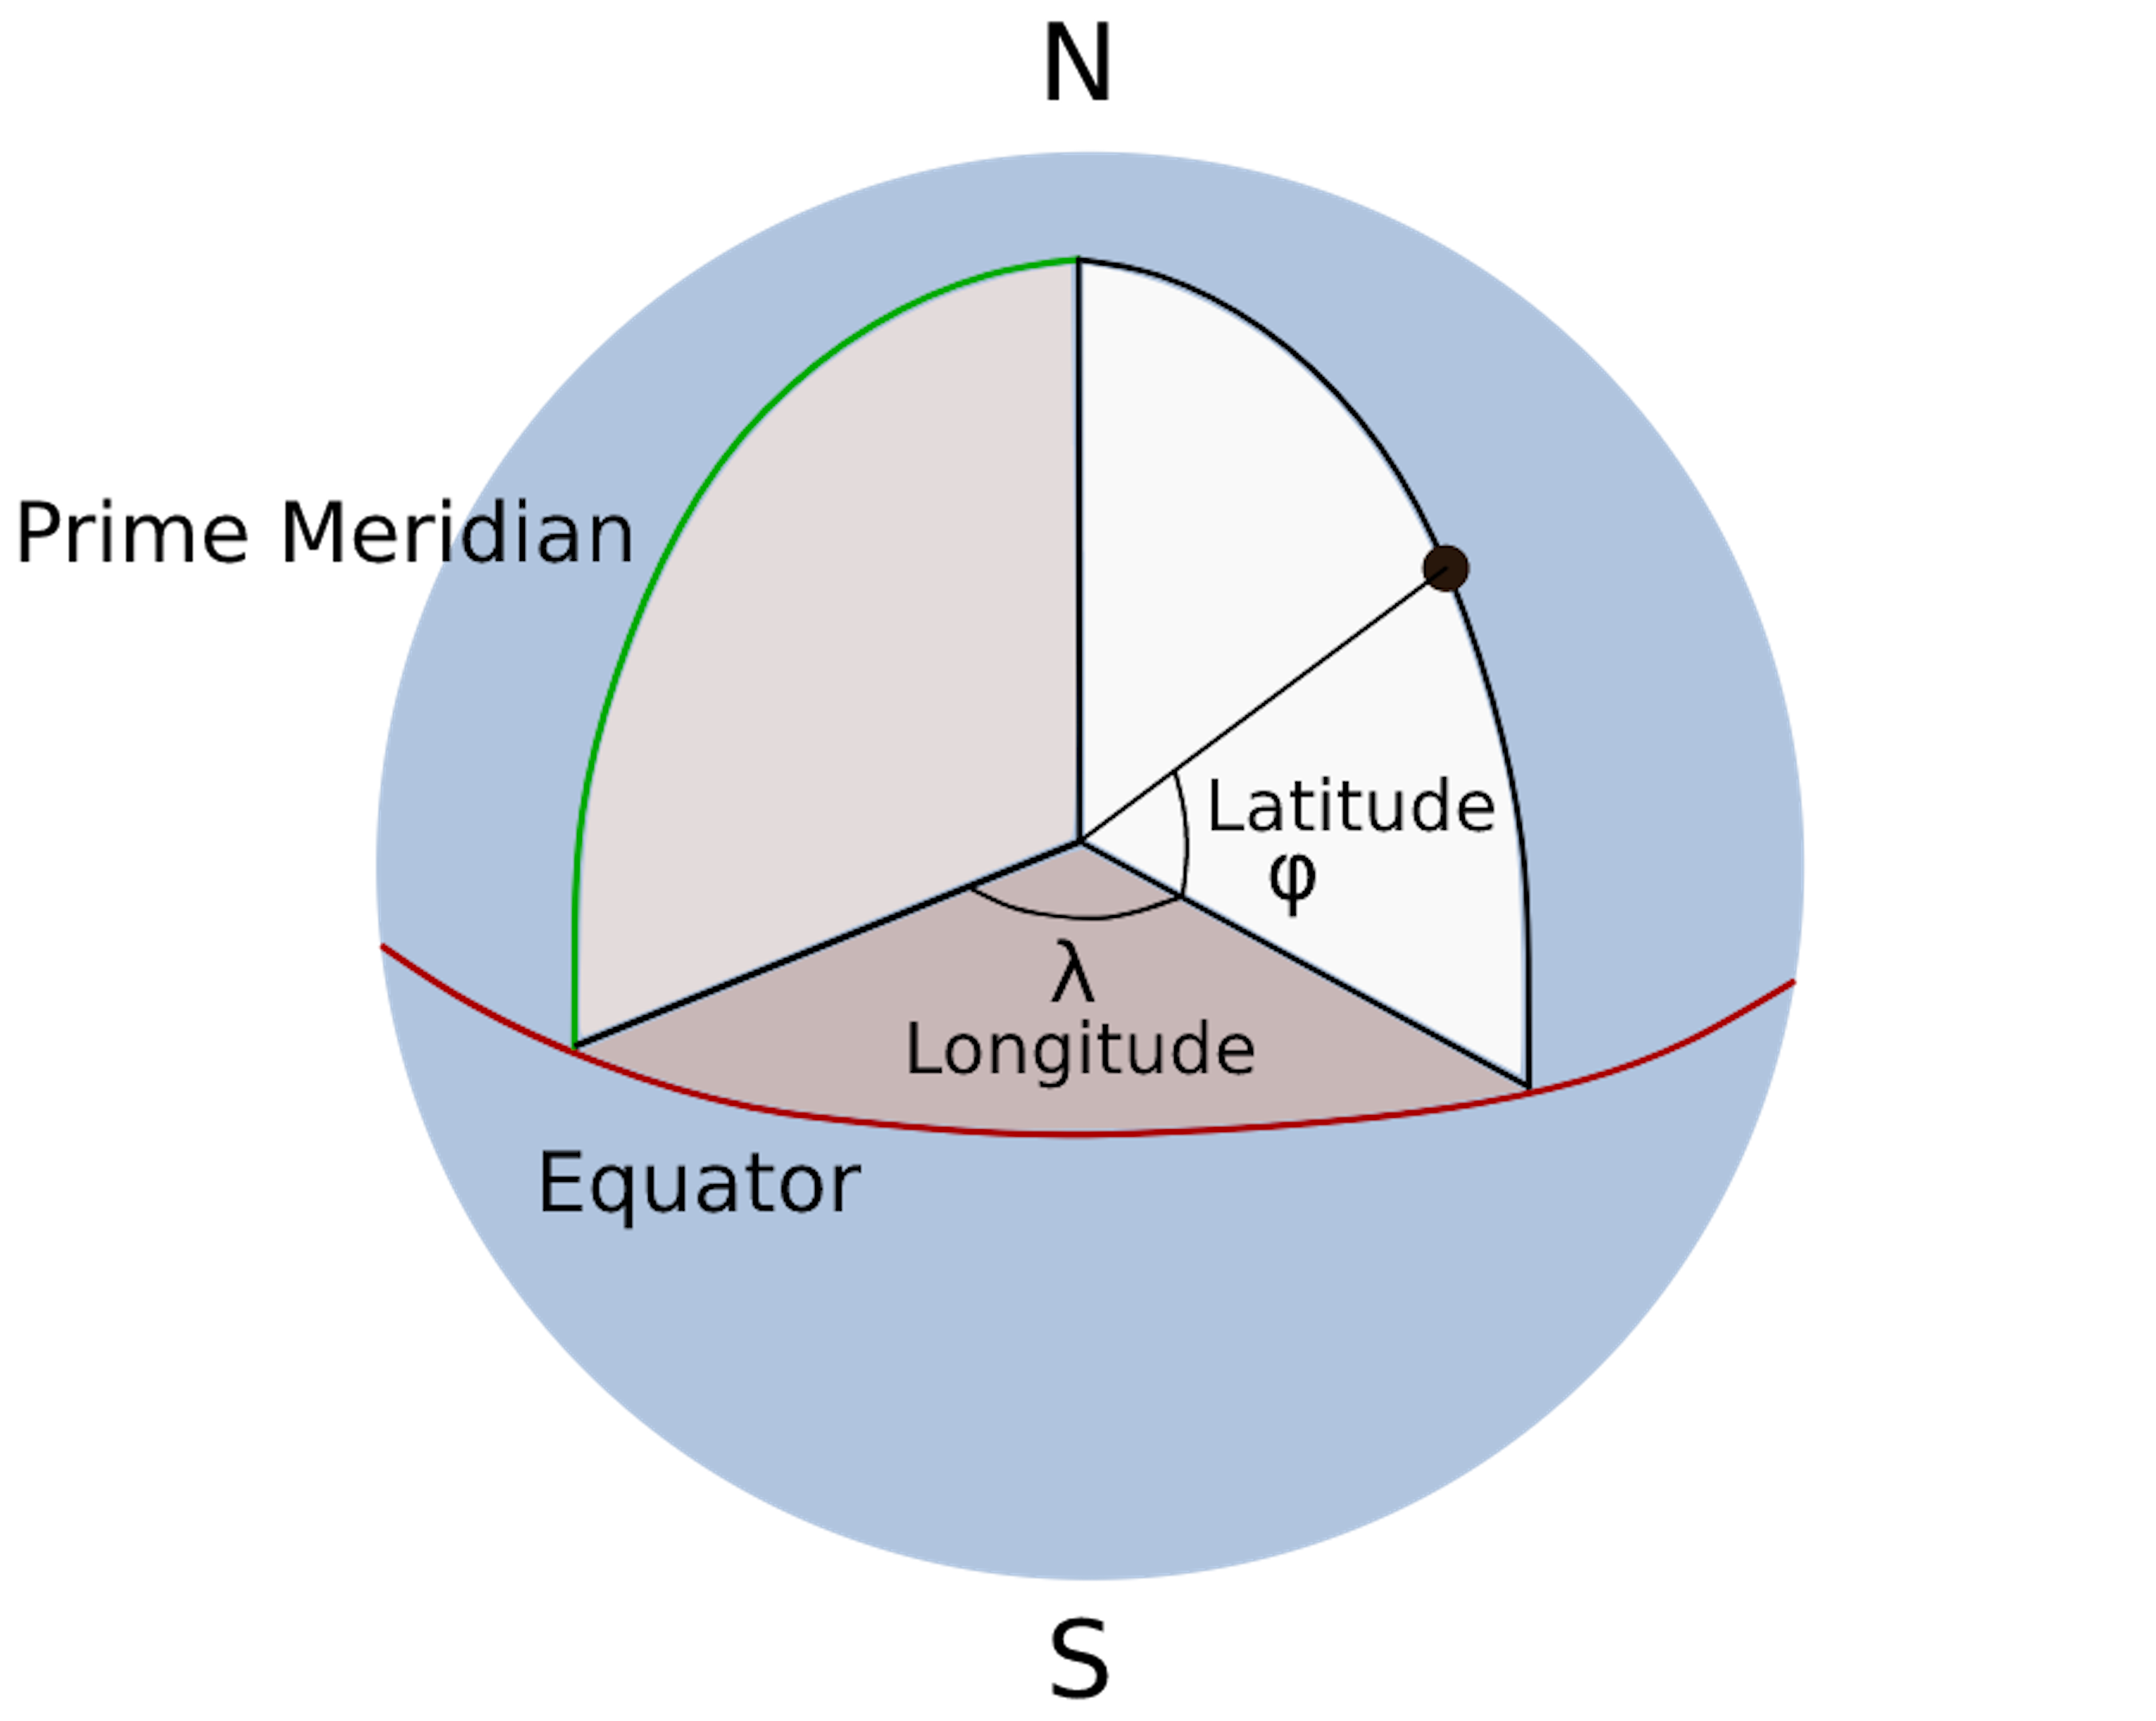
\includegraphics[width=0.9\textwidth]{Figures/latlong.png}
%   \caption[Illustration of latitude and longitude]{Illustration of the earth, and how latitudes and longitudes are calculated with respect to the equator and the prime meridian.}
%   \label{fig:latlong}
% \end{figure}


% \subsection{How to access tables and figures from the Simulation study}
% Here is a table for a single covariance level:
% % latex table generated in R 4.2.1 by xtable 1.8-4 package
% Thu Dec 14 12:52:54 2023
\begin{table}[ht]
\centering
\begin{tabular}{lrrr}
  \hline
Method & Mean & Quantile\_2.5 & Quantile\_97.5 \\ 
  \hline
Relaimpo & 0.125211 & 0.116182 & 0.133762 \\ 
  BVI & 0.125146 & 0.117180 & 0.133329 \\ 
  ELMG & 0.125138 & 0.117082 & 0.133092 \\ 
  ERW & 0.125130 & 0.117086 & 0.133242 \\ 
   \hline
\end{tabular}
\end{table}


% Here is one of the violin plots. The formatting of these might need som altering as it does not appear to nice right now. 
% \begin{figure}[ht]
%     \centering
%     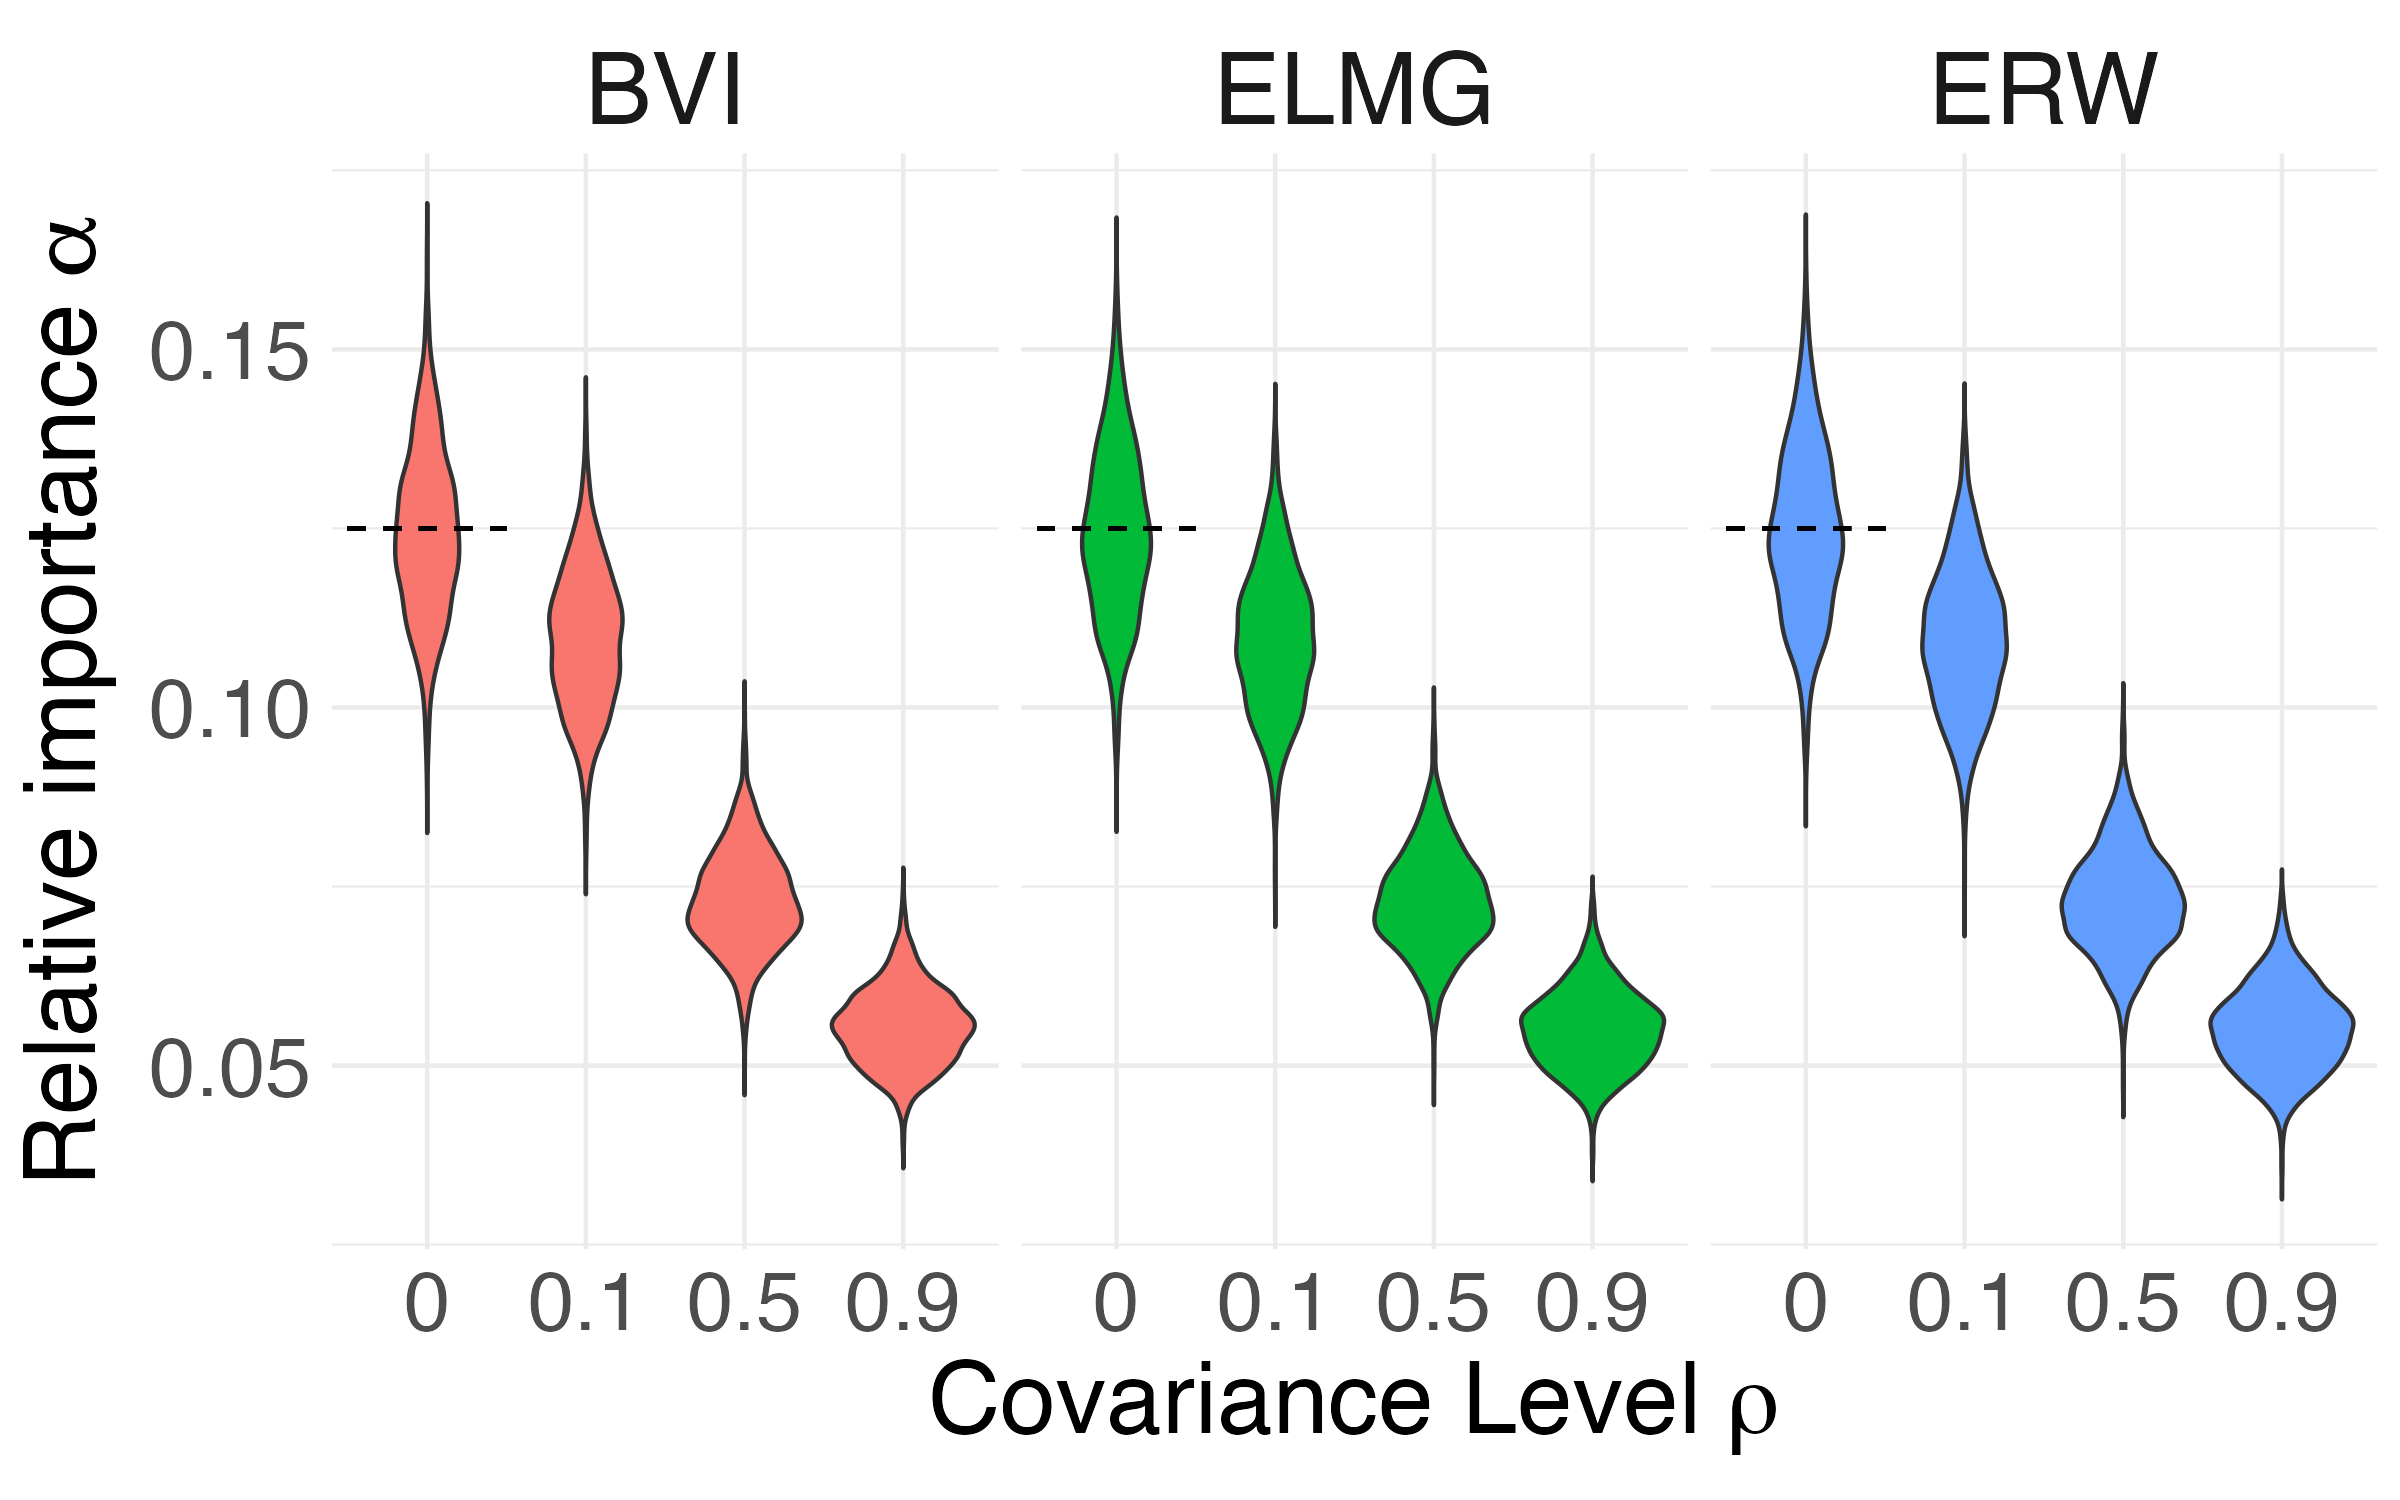
\includegraphics[width=\linewidth]{Figures/ViolinPlots/Variance_gamma.png}
%     \caption{Caption for the figure.}
%     \label{fig:my_label}
% \end{figure}



% \subsection{Citations}
% Here are some examples on how to reference a source (where none is relevant to the text but just for illustration purposes only). One may citet a single reference by calling \citet{wolves_of_mount_mckinley}, or several in the same bracket by calling \citet{machine_learning, clustering_impossibility} when they are all related to the same statement. There are many different styles on how to citet, and how the layout and order of your citation style is presented. This is my favorite, as I find it neat and tidy \citet{sheep}. It will show up in order of appearance in the references section.
\cleardoublepage

%Regarding theory chapter:
%Need to decide if we back transform via lambda or not
%Need some feedback on the theory to make everything correct. 
%More specifically chapters 2.1, 2.5 and 3.1


\chapter{Methods}
\label{ch:method}
\section{Variable importance in a Bayesian framework}
\label{sec:implementation}
We now propose a method for calculating relative variable importance in a Bayesian framework, which we call Bayesian Variable Importance (BVI). 
The BVI method is based on the idea that the relative weights approach, introduced in \Cref{sec:relativeweights}, combined with its extension \citep{matre} can be used to fit a Bayesian LMM.
With this basis we believe that it is possible to create a Bayesian relative importance measure, by taking the new framework into account.
%The BVI method is based on the relative weights approach introduced in \Cref{sec:relativeweights} and extended by \citet{matre}, to fit a Bayesian LMM using INLA, which is described in \Cref{sec:INLA_framework}.
When considering the fixed effects there are multiple established methods to compare results with. Here, we compare our results to the previously discussed methods LMG \citep{gromping_relaimpo}, the extended LMG (ELMG) and the extended relative weights (ERW) \citep{matre}.
The ELMG and the ERW are extensions of the LMG and relative weights methods respectively, to be compatible with the linear mixed models.
This thesis will focus on linear mixed models containing only random intercepts. 
More general methods with random slopes and GLMM's with a link function not corresponding to a normal distribution are not in the scope of this thesis.

\subsection{Relative variable importance calculations}
First, we must incorporate the matrix transformation from the relative weights method for the Bayesian framework.
The orthogonal matrix $\mathbf{Z}$ is generated from only the fixed effects $\mathbf{X}$, which corresponds to the variables for the fixed effects also in the Bayesian framework. Therefore, we can apply this transformation before the Bayesian analysis is performed.
This transformation includes standardizing the data to be centered around zero and a standard deviation of one unit variance, as well as orthogonalizing the design matrix.
\newline
\newline
The variance decomposition of the random intercept model takes the form
%The variance decomposition of the above explained model using $\mathbf{Z}$ is
\begin{equation}
    \text{Var}(\mathbf{y}) = \text{Var}(\mathbf{X}\boldsymbol{\beta}_{\mathbf{X}} + \mathbf{U}\boldsymbol{\alpha} + \boldsymbol{\varepsilon}) = \boldsymbol{\beta}_{\mathbf{X}}^T\text{Var}(\mathbf{X})\boldsymbol{\beta}_{\mathbf{X}} + \mathbf{U}\mathbf{G}\mathbf{U}^T + \sigma_{\varepsilon}^2\mathbf{I} = 1  \ ,
    \label{eqn:Variance_random}
\end{equation}
where $\mathbf{U}$ is now a sparse block matrix where each block $\mathbf{U}_j \in \mathbb{R}^{n_j \times q}$ is a matrix of ones, $n_j$ the number of observations in cluster $j$, $q$ the number of random intercepts and $\mathbf{G}$ is a blockdiagonal matrix with $\mathbf{Q}$ on the diagonal.
In the special case of an independent and identically distributed (iid) random intercept model, this variance decomposition can be simplified.
With several, independent random intercepts, each intercept $\boldsymbol{\alpha}_j$ contributes $\sigma^2_{\alpha_j}$ to the total model variance, making $\mathbf{G}$ a diagonal matrix, so the total variance of the model can be decomposed as
\begin{equation}\label{eq:variance_theoretical_x}
    \text{Var}(\mathbf{y}) = \sum_{i=1}^p \beta_{i, \mathbf{X}}^2 v_{i, \mathbf{x}_i} + 2 \sum_{i=1}^p \sum_{k=i+1}^p \beta_{i, \mathbf{X}}\beta_{k, \mathbf{X}}\sqrt{v_{i, \mathbf{x}_i}v_{k, \mathbf{x}_k}}\rho_{ik} + \sum_{j=1}^q \sigma^2_{\alpha_j} + \sigma^2_{\epsilon} = 1 \ ,
\end{equation}
where $\beta_{i, \mathbf{X}}$ is the vector of regression coefficients when regressing $\mathbf{y}$ on $\mathbf{X}$, $v_{i, \mathbf{x}_i}$ is the variance of the $i$'th column $\mathbf{x}_i$ and $\rho_{ik}$ is the correlation between the $i$'th and $k$'th columns. 
However, with the relative weights method, we approximate the design matrix $\mathbf{X}$ with the orthogonal matrix $\mathbf{Z}$. 
Consequently, the variance of each column in $\mathbf{Z}$, $v_{i, \mathbf{z}_i}$, is equal to one and the correlation $\rho_{ik}$ between the columns is zero. 
Therefore, the total variance in \eqref{eq:variance_theoretical_x} can be approximated by
\begin{equation}\label{eq:variance_rw}
    \text{Var}(\mathbf{y}) \approx \sum_{i=1}^p \beta_{i, \mathbf{Z}}^2 + \sum_{j=1}^q \sigma^2_{\alpha_j} + \sigma^2_{\epsilon} \ ,
\end{equation}
where $\beta_{i, \mathbf{Z}}$ is the vector of regression coefficients when regressing $\mathbf{y}$ on $\mathbf{Z}$, $\beta_{i, \mathbf{Z}}^2$ represents the variance of column $\mathbf{z}_i$, $\sigma_{\alpha_j}^2$ the variance of $\boldsymbol{\alpha}_j$ and $\sigma^2_{\varepsilon}$ the variance of $\boldsymbol{\varepsilon}$.
To map the importances of each column in $\mathbf{z}_i$ back to the importance of the columns $\mathbf{x}_i$, we regress $\mathbf{Z}$ on $\mathbf{X}$ to obtain the matrix $\boldsymbol{\Lambda}$ as in \Cref{sec:relativeweights}.
The final model variance obtained from this setup, can then be estimated as 
\begin{equation}
    \label{eq:variance_calc}
    \text{Var}(\mathbf{y}) \approx \sum_{i=1}^p \text{RI}(\mathbf{x}_i) + \sum_{j=1}^q \sigma^2_{\alpha_j} + \sigma^2_{\epsilon} \approx \sum_{i=1}^p (\Lambda^{[2]}\beta_{\mathbf{Z}}^{[2]})_i + \sum_{j=1}^q \sigma^2_{\alpha_j} + \sigma^2_{\epsilon} \ ,
\end{equation}
where $\mathbf{x}_i$ is column $i$ of $\mathbf{X}$.  
Since the response is standardized the relative importance, or proportion of variance explained, of regressor $X_i$ is given by $\Lambda^{[2]}\beta_{\mathbf{Z}}^{[2]}$ and the relative importance of random intercept $\boldsymbol{\alpha}_j$ is given by $\sigma^2_{\alpha_j}$.
\subsection{Handling the model fit with INLA}
\label{sec:BVI_handling}
Once $\mathbf{Z}$ has been created from the projection of $\mathbf{X}$ into the orthogonal space, a model of the response, which has the form as explained in \Cref{sec:LMM}, is fit using $\mathbf{Z}$ as the design matrix and INLA. 
INLA is our preferred computational tool to fit the Bayesian LMM since it is very efficient, especially for large data sets and complex models.
After the model is fit, INLA provides the approximate marginal posterior distribution of each component in $\boldsymbol{\beta}_{\mathbf{Z}}$, the precision of $\boldsymbol{\alpha}$, the precision of $\boldsymbol{\varepsilon}$ and allows us to sample from the joint posterior distribution $\pi(\boldsymbol{\beta}_{\mathbf{Z}}, \boldsymbol{\alpha}, \boldsymbol{\varepsilon} \lvert \mathbf{y})$. 
Since each random intercept and the random errors are assumed to be iid, the marginal distributions of the precisions represent the full distributions of the precisions. 
The respective distributions are then inverted, so that they correspond to the distribution of the variances for $\boldsymbol{\alpha}$ and $\boldsymbol{\varepsilon}$. 
Since the response is standardized, these variance distributions correspond to a distribution of the proportion of variance explained by each random intercept, i.e. a distribution of their relative importance.
For the fixed effects, samples of $\boldsymbol{\beta}_{\mathbf{Z}}$ from the joint posterior are drawn, squared and transformed with \eqref{eq:RI_lambda}, to represent a sampled distribution of the individual relative importance. 
We must sample $\boldsymbol{\beta}_{\mathbf{Z}}$ from the approximate joint distribution since the marginal distributions only describe the behavior of individual components of $\beta_{i, \mathbf{Z}}$ in isolation, and therefore does not take correlation between them into account.
Using INLA functionality, for a sample $\boldsymbol{\beta}_{s, \mathbf{Z}}$ from the approximate joint distribution we can estimate the relative importance for each column in $\mathbf{X}$ by
\begin{equation}
    \text{RI}(\mathbf{X})_s = \boldsymbol{\Lambda}_{s}^{[2]} \boldsymbol{\beta}_{s, \mathbf{Z}}^{[2]} \ ,
\end{equation}
where, $\text{RI}(\mathbf{X})_s$ is a column vector where entry $j$ is the estimate of the relative importance of column $j$ in $\mathbf{X}$ from the sample $\boldsymbol{\beta}_{s, \mathbf{Z}}$.
By repeating this process for multiple samples, one can obtain an estimate of the posterior distribution of each element in $\text{RI}(\mathbf{X})$.
From the estimated posterior distribution of elements in $\text{RI}(\mathbf{X})$ and the marginal distributions of $\boldsymbol{\alpha$ and $\boldsymbol{\varepsilon}}$ we can obtain the model $R^2$ distribution in the Bayesian framework as described by equations \eqref{eq:R2_bayes_LMM_cond} and \eqref{eq:R2_bayes_LMM_marg}.
The advantage of having the posterior distributions instead of point estimates is prominent in natural sciences where one might have complex data structures, since it carries a fundamental uncertainty.
% I dont know where to place the above sentence, but I think it is important to mention!!!!!!



% \section{Extending the relative weights method to the Bayesian linear regression with random intercepts}
% %Need a review of this section!
% The relative weights method proposes a transformation to the covariates in a linear regression. Since the same covariates would also be considered to be fixed effects in a Bayesian setting, one can apply the relative weights transformation to the design matrix $\mathbf{X}$ also in a Bayesian framework.
% After obtaining the orthogonal matrix $\mathbf{Z}$, random effects $\boldsymbol{\alpha}$ that are assumed independent of the fixed effects can be introduced. 
% A model can now be fit with the matrix $\mathbf{Z}$ containing the fixed effects and $\boldsymbol{\alpha}$ as the random effects.
% If one now in addition standardizes the response of this model, the proportion of variance explained by each fixed and random effects can be 
% These would contribute to the model variance as described in sections \ref{sec:R2_LMM} and \ref{sec:bayes_R2_LMM}.


% %NEED TO DECIDE IF WE BACK TRANSFORMS THE IMPORTANCES VIA $\boldsymbol{\Lambda}$ OR NOT. 
% \begin{equation}
%         \text{Var}(\mathbf{y}) = \text{Var}(\mathbf{Z}^T\boldsymbol{\beta}_{\mathbf{Z}} + \mathbf{U}\boldsymbol{\alpha} + \boldsymbol{\varepsilon}) = \boldsymbol{\beta}_{\mathbf{Z}}^T\text{Var}(\mathbf{Z})\boldsymbol{\beta}_{\mathbf{Z}} + \mathbf{U}\mathbf{G}\mathbf{U}^T + \sigma_{\varepsilon}^2\mathbf{I}  \ .
%         \label{eqn:Variance_random}
% \end{equation}
% Now a few simplifications can be made for the random intercept model. The matrix $\mathbf{Z}$ now has variance equal to one, the random intercepts are pairwise independent and we have scalar variances for each random intercept. Taking into consideration the form that $\mathbf{U}$ takes for the random intercept model, we can decompose the conditional variance as 
% \begin{equation} \label{eqn:Variance_random_intercept}
%     \text{Var}(\mathbf{y}) = \text{Var}(\mathbf{Z}^T\boldsymbol{\beta}_{\mathbf{Z}} + \mathbf{U}\boldsymbol{\alpha} + \boldsymbol{\varepsilon}) = \boldsymbol{\beta}_{\mathbf{Z}}^T\boldsymbol{\beta}_{\mathbf{Z}} + \mathbf{U}\mathbf{G}\mathbf{U}^T + \sigma_{\varepsilon}^2\mathbf{I}  \ .
% \end{equation}
% where $\mathbf{U}$ is now a sparse block matrix where each block $\mathbf{U}_j \in \mathbb{R}^{n_j \times q}$ is a matrix of ones with size and $\mathbf{G}$ is a diagonal matrix with $\mathbf{G}_{jj} = \sigma_{\alpha_j}^2$. The resulting matrix $\mathbf{U}\mathbf{G}\mathbf{U}^T$ contains the variance of all random intercepts in the model along its diagonal.
% The \texttt{R-INLA} package allows us to model this as well as sample from the posterior distribution of all variance components.
% Thus if one performs the transformation of $\mathbf{X}$ through the relative weights method, and applies INLA with the design matrix $\mathbf{Z}$ along with the random effects, we are able to decompose the variance of the model following \eqref{eqn:Variance_random_intercept}.




%. To calculate the relative variable importance(RVI) we use the posterior mean of the coefficients $\boldsymbol{\beta}$ and $\boldsymbol{\alpha}$ and calculate the RVI for each fixed effect as
%\begin{equation}
%    \text{RVI}_i = \frac{\beta_i^2}{\text{Var}(y)} \hspace{5mm} i=1, ..., p \ ,
%\end{equation}
%and for each random intercept as 
%\begin{equation}
%    \text{RVI}_j = \frac{\sigma^2_{\alpha_j}}{\text{Var}(y)} \hspace{5mm} j=1, ..., q \ .
%\end{equation}
%Using the posterior means allow for easier comparisons with the LMG and relative weights methods


% Write more about the possibility of obtaining a posterior distribution of the variance explained?


%Should I do the simulation study again, but with different regression coefficients and some negative correlation?

\section{Simulation study}
\label{sec:simulations}
To evaluate the performance of our proposed method, BVI, a simulation study was conducted. The study investigates how the BVI compares to the relative importance decomposition(Relaimpo) presented in \citet{gromping_relaimpo} and the two methods presented in \citet{matre}.
The Relaimpo method uses the LMG decomposition and considers only fixed effects and can therefore only be compared with the BVI in the fixed effects. The two methods in \citet{matre}, ELMG and the ERW, are extensions of the LMG and relative weights methods respectively, to include random intercepts.
These extensions allow us to compare the results for the random intercept model to our BVI method. The decompositions of the variance in \eqref{eq:variance_theoretical_x} can be used to compare the theoretical variance explained in a model against the results from Bayesian Variable Importance method.
Since the response $\mathbf{y}$ is standardized, each relative importance assigned to a distinct effect is analogous to a proportion or percentage of the total variance of $\mathbf{y}$.
\newline
\newline
To simulate the data we consider the model as in \eqref{eq:LMM}, with a sample size $n=10^4$, $\boldsymbol{\alpha}=(\alpha_1, ..., \alpha_m)$ where $\alpha_i \stackrel{iid}{\sim} \mathcal{N}(0, \tau^2=1)$ as a single random intercept for $m=200$ clusters of $n_j=50$ observations each, $\mathbf{X} \sim \mathcal{N}(\boldsymbol{\mu},\Sigma) \in \mathbb{R}^{n \times p}$, where $\boldsymbol{\mu}=(1, 2, 3)$, $\Sigma_{ii} = 1, \Sigma_{i, k}=\rho_{i, k}, k\neq i$ and $p=3$ consisting of three fixed effects, $\mathbf{U}$ as a desgin matrix of appropriate dimension and a random error $\varepsilon_i \stackrel{iid}{\sim} \mathcal{N}(0, \sigma^2=1)$. 
Further, the true vector of regression coefficients is set to be set to be $\boldsymbol{\beta}_{\mathbf{X}}=(1, \sqrt{2}, \sqrt{3})^T$ so the total model, including an intercept column of ones, can be written as
\begin{equation}
    \label{eq:simulation_model}
    \mathbf{y} = \mathbf{1} + \mathbf{X}\boldsymbol{\beta}_{\mathbf{X}} + \mathbf{U}\boldsymbol{\alpha} + \boldsymbol{\varepsilon} \ ,
\end{equation}
The data is standardized, meaning that $\sigma^2_{\mathbf{y}}=1$, $\boldsymbol{\beta}_{\mathbf{X}}=(\sqrt{1/8}, \sqrt{2/8}, \sqrt{3/8})^T$ and $\sigma^2_{\alpha}=\sigma^2_{\varepsilon} = 1/8$.
This standardization allows us to easily compare and interpret results as proportions of the total variance of $\mathbf{y}$.
\newline
\newline
From this setup, the theoretical variance of the response is
\begin{equation}
    \label{eq:variance_theoretical_simulation}
    \text{Var}(\mathbf{y}) = \beta_{1, \mathbf{X}}^2 + \beta_{2, \mathbf{X}}^2 + \beta_{3, \mathbf{X}}^2 + 2\sum_{j=1}^{3}\sum_{k=j+1}^{3} \beta_{j, \mathbf{X}}\beta_{k, \mathbf{X}}\rho_{jk} + \sigma_{\alpha}^2 + \sigma^2_{\varepsilon} \ .
\end{equation}
as in \eqref{eq:variance_theoretical_x} and the theoretically correct relative importances for uncorrelated data are
\begin{equation}
    \begin{aligned}
        \text{RI}(\mathbf{x}_1) =  \beta_{1, \mathbf{X}}^2& = \text{RI}(\alpha) = \sigma^2_{\alpha} = \frac{1}{8} \hspace{1mm}, \hspace{1mm} \text{RI}(\mathbf{x}_2) = \beta_{2, \mathbf{X}}^2 = \frac{2}{8} \hspace{1mm}, \hspace{1mm} \text{RI}(\mathbf{x}_3) = \beta_{3, \mathbf{X}}^2 = \frac{3}{8} \ . 
    \end{aligned}
\end{equation}
Further, the theoretically expected marginal and conditional $R^2$ values can be calculated from \ref{eq:variance_theoretical_simulation} as the variance of the fixed effects divided by the total variance and the variance of the fixed effects and random intercepts divided by the total variance respectively. 
The $R^2$ values are listed in \Cref{table:1}.
\begin{table}[ht]
    \centering
    \begin{tabular}{lrr}
    \hline
    $\rho$ & $R^2_{\text{marg}}$ & $R^2_{\text{cond}}$\\ 
    \hline
    $0$ & $0.750$ &  $0.875$ \\ 
    $0.1$ & $0.781$ & $0.890$ \\ 
    $0.5$ & $0.852$ & $0.926$\\ 
    $0.9$ & $0.889$ & $0.945$\\ 
    \hline
    \end{tabular}
    \caption{The theoretically correct marginal variance explained (left column) and conditional variance explained (right column) for different correlation levels between the fixed effects.}
    \label{table:1}
\end{table}
These values provide an empiric way of checking if our method fulfills the proper decomposition criteria listed in \Cref{sec:rel_imp}, by seeing if the relative importances for each effect sum to the model $R^2$.
\newline
To investigate how different correlations between the fixed effects are handled by the method, we consider four different correlation levels between the fixed covariates in our data. That is achieved by letting $\rho_{1, 2} = \rho_{1, 3} = \rho_{2, 3}$ take on the values $\{0, 0.1, 0.5, 0.9$\}.
For each correlation level, we simulate $N=1000$ datasets and fit each of the four methods BVI, Relaimpo, ELMG and ERW.
To get a comparable measure from the Bayesian framework to the frequentist framework, we use the posterior means of the sampled posterior distribution of $\text{RI}(\mathbf{X})$ when estimating \eqref{eq:variance_calc}.
It can here be noted that in the BVI method the approximated posterior marginals for each predictor, as well as the sampled posterior distribution of $\boldsymbol{\beta}_{\mathbf{Z}}$ and $\text{RI}(\mathbf{X})$, are available for each dataset. 


% To easily compare the BVI method with the Relaimpo, the ELMG and ERW methods in the frequentist framework, one can insert the posterior means or modes of the estimates for $\beta_i$ and the variances of $\alpha_j$ and $\varepsilon$ in \eqref{eq:variance_rw}.
% However, more inference can be made since we have the marginal posterior distribution of each component.





\cleardoublepage

\chapter{Results}
\label{ch:results}
% \section{Relative weights accuracy}

% \section{Posterior distributions compared to proportion of variance explained}

% I picture running a linear regression model with different correlation values for two, three and maybe 4 covariates and discuss the effects of this.

% \subsection{Linear regression}
% \subsubsection{Analytical solutions}
% \subsubsection{Impact of correlated data}

% \subsection{Linear regression with a random intercept}

% \subsection{Linear regression with two or more random intercept}

% \subsection{LMM's?}

% \subsection{Analytical solutions(if included)}

% \section{Interpretations, findings and $R^2$}
\section{Insights from the simulation study}
To present the results of the simulation study we consider each effect separately in different plots, that is we show results for the importance of variables $X_1, X_2, X_3$ and the random effect $\boldsymbol{\alpha}$, in distinct plots. 
We used violin plots to visualize the estimated quantities, as they contain much information in a compact way. The violin plot is analogous to a density plot, but the density is shown along the $y$-axis and mirrored about the $y$-axis to form a symmetrical shape. Each violin therefore displays the distribution of our simulated estimates.
Lastly, we consider how our BVI model estimates the conditional and marginal $R^2$ values from a Bayesian perspective, comparing these results to the $R^2$ value obtained from the decompositions by the Relaimpo, ELMG, and ERW methods, where the first method only considers models without random effects. 
\subsection{Relative importance of the fixed effects}
\label{sec:relimp_fixed}
In \Cref{fig:relimp_X1,fig:relimp_X2,fig:relimp_X3} the distribution of the relative importance allocated to each fixed effect from the simulations are shown.
There are four different distributions for each method, which corresponds to the four different correlation levels. 
The horizontal dashed line displays the theoretically correct relative importance when the covariates are pairwise independent. 
\newline
\newline
In general, it can be seen that the distributions in the case of uncorrelated data are unbiased with some variation around the theoretically correct relative importance.
For a correlation of $\rho=0.1$ the distributions of the estimates are shifted marginally compared to the uncorrelated case for all methods.
The importance attributed to $X_1$ and $X_2$, in \Cref{fig:relimp_X1}a and \Cref{fig:relimp_X2}b respectively, is larger when compared to the uncorrelated case, whereas the importance attributed to $X_3$ in \Cref{fig:relimp_X3}c is smaller.
All methods seem to shift the relative importance estimate for the covariate with the same amount in the same direction.
This shift is both expected and desirable, when considering the values found in \Cref{table:1} for the theoretically correct variance explained. 
Therefore, we should expect our method to assign different shares when we have various levels of covariate correlation, which it does.
This trend continues for the correlation level $\rho=0.5$, where the distributions are shifted further in the same directions as for $\rho=0.1$.
Lastly, for $\rho=0.9$ we see the largest reallocation of the distributions, which follows the same trend as for the other correlation levels.
\newline
\newline
The rise in importance for $X_1$ and $X_2$ for increasing correlation can be understood by the relation $\mathbf{Z}\boldsymbol{\Lambda}=\mathbf{X}$ in the relative weights method. 
When the matrix $\mathbf{X}$ is not correlated, $\boldsymbol{\Lambda}$ is close to the identity matrix, but with an increase in correlation the diagonal elements grows smaller and off diagonal elements grow larger.
An increase in off diagonal values would for $X_1$ and $X_2$ imply that a larger value is multiplied with $\beta_3^2$, which is larger than $\beta_1^2$ and $\beta_2^2$. 
Therefore, it is expected to see a rise in importance as correlation increases for $X_1$ and $X_2$, and the opposite for $X_3$.
In all figures, the BVI method is in agreement with the other methods when allocating importance for different correlation levels.
The width of the distributions seem to become lower as the correlation increases, most notably for $\rho=0.9$, where the distributions exhibit significantly smaller dispersion than for $\rho=0$.
Generally all methods seem to follow the same trends and produce similar results for all three fixed effects. 
As correlation increases the trend is that the relative importance assigned to $X_1$ and $X_2$ increases, in contrast to the decrease in relative importance assigned to $X_3$.
\newline
\newline
In general, the BVI method is in agreement with the theoretical results for uncorrelated data derived in \Cref{ch:method} and is consistent with the other three methods for correlated fixed effects. 
\begin{figure}[H]
  \centering
    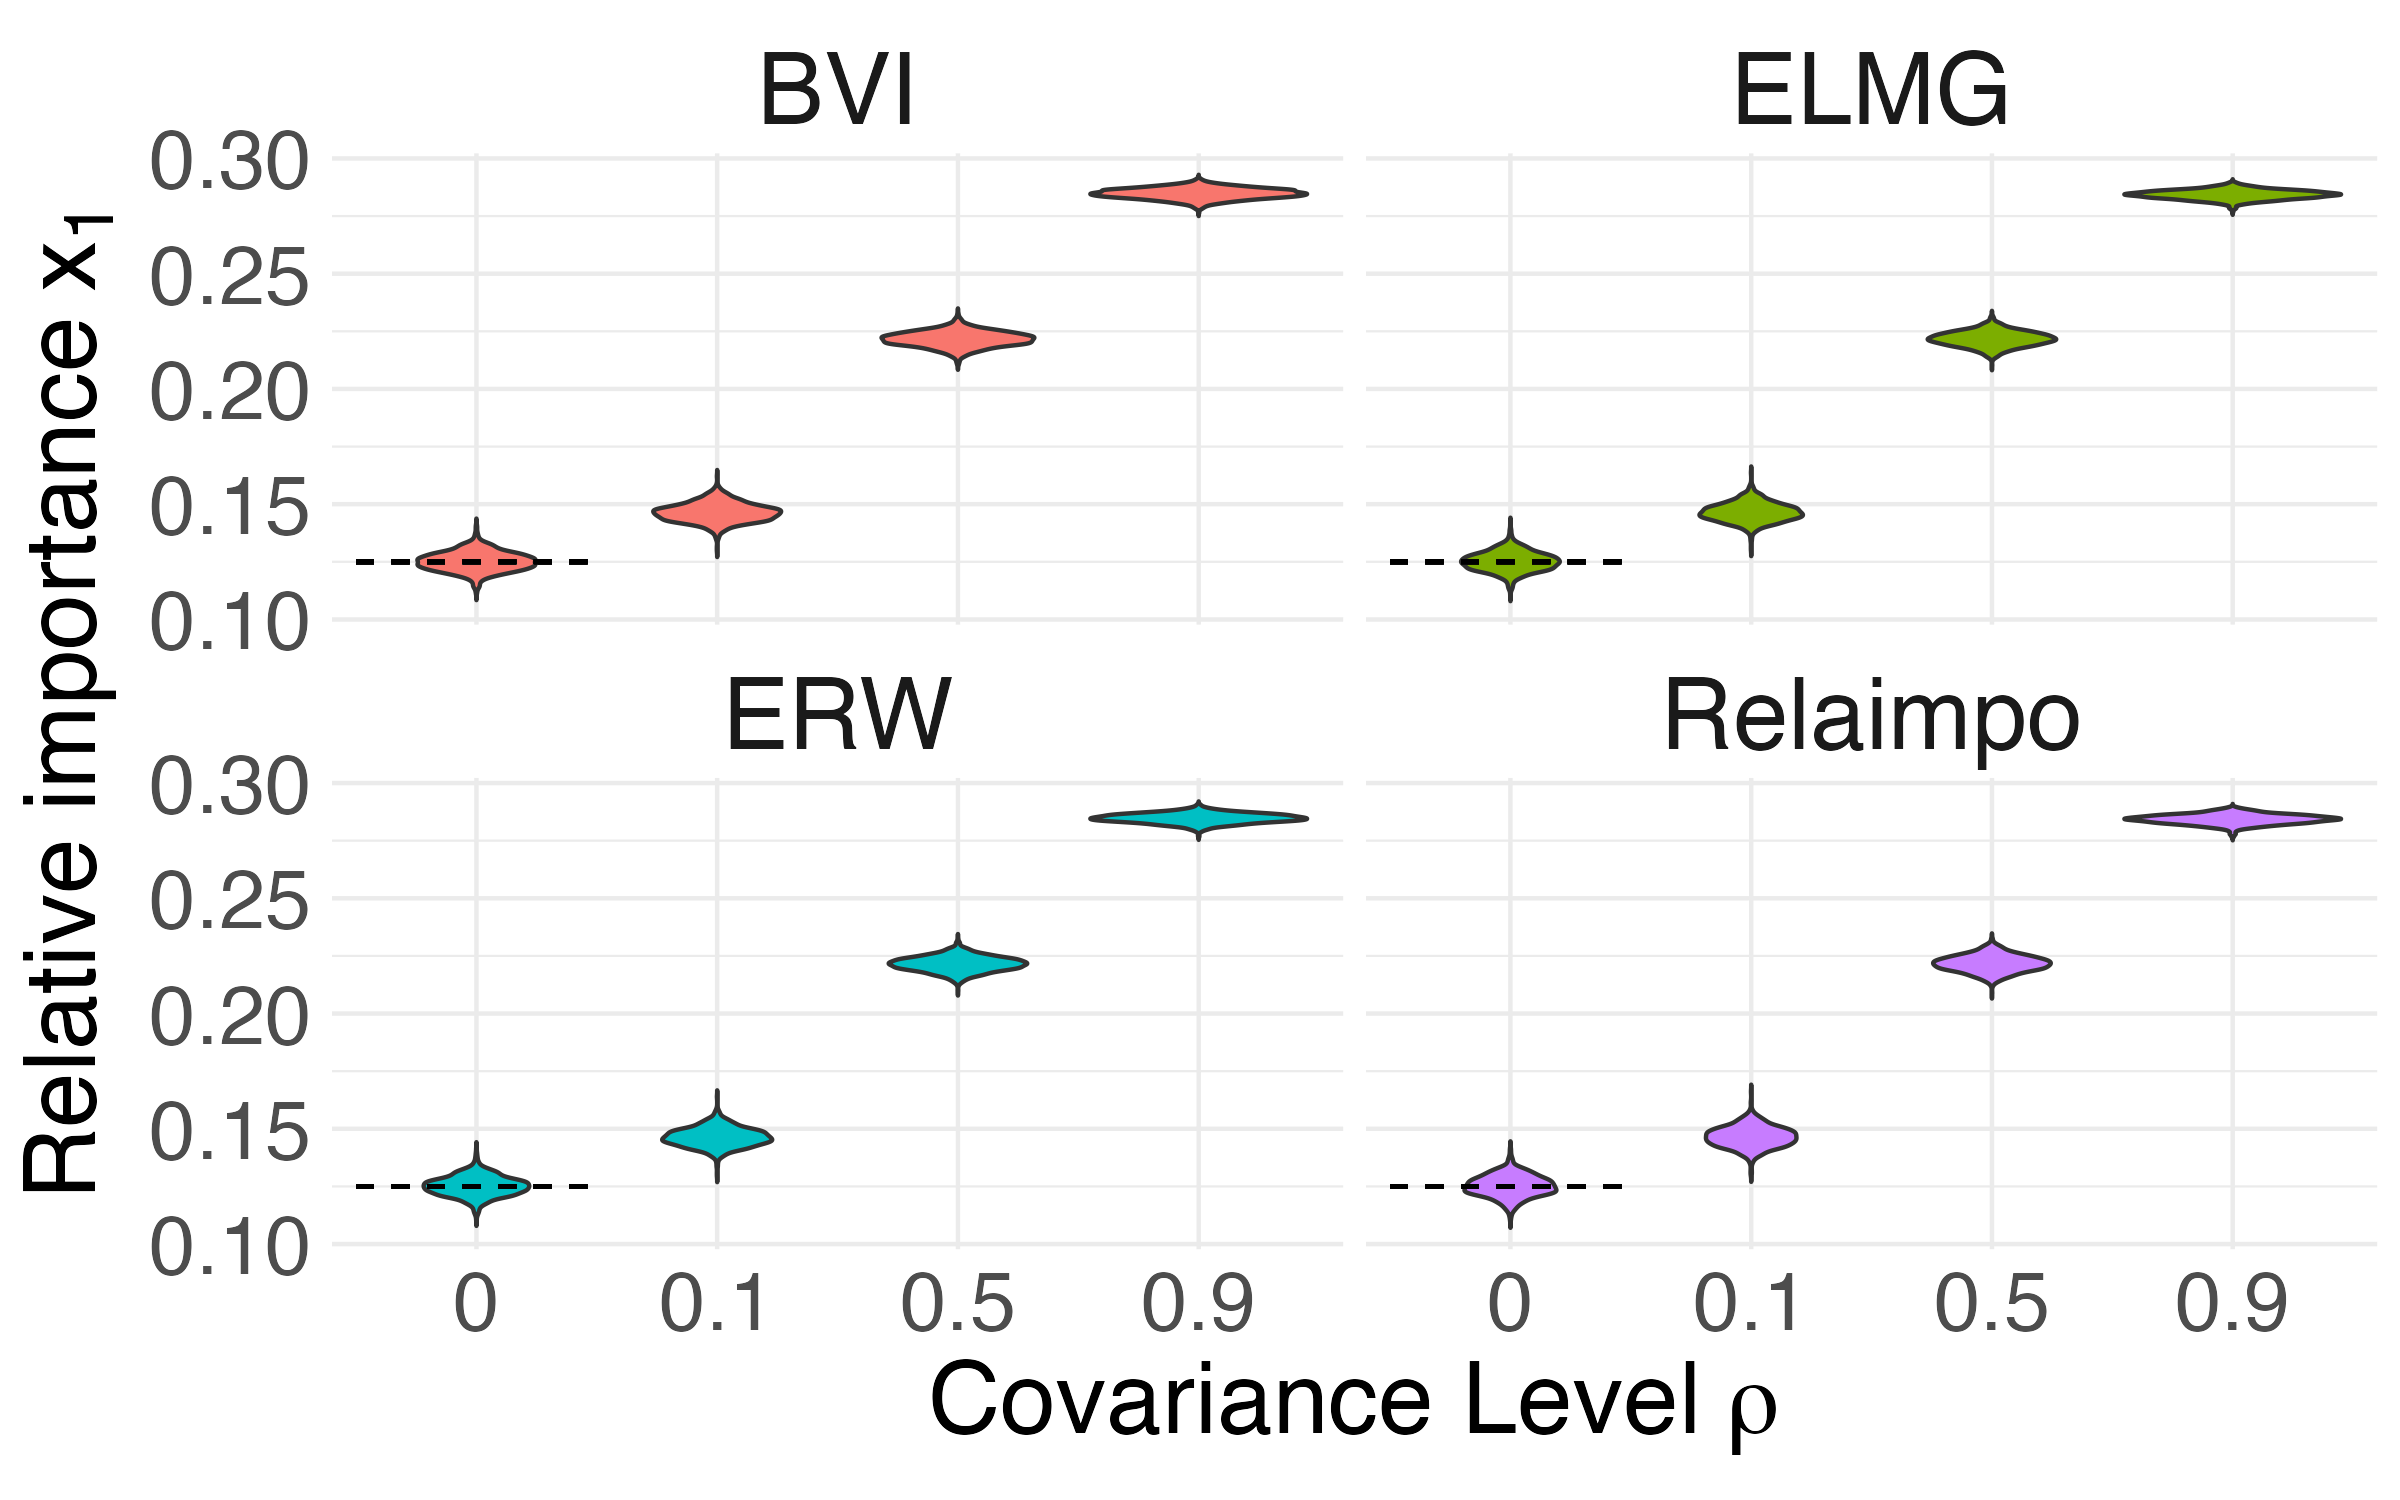
\includegraphics[width=0.7\linewidth]{Figures/ViolinPlots/Variance_V1.png}
    \caption{Violin plots for the relative importance of the fixed effects $X_1, X_2$ and $X_3$ for different correlation levels calculated from the ensemble of simulated datasets by the BVI, ELMG, ERW and the Relaimpo methods. The standardized regressor coefficients are $\boldsymbol{\beta}=\left(\sqrt{1/8}, \sqrt{2/8}, \sqrt{3/8}\right)$, and the true total model variance is $\sigma^2_{\mathbf{y}}=1$. For the BVI method the distributions of posterior means are shown to compare to the distribution of point estimates from the other three methods. The horizontal line displays the theoretically correct importance of each fixed effect in the case of uncorrelated data. (a) Relative importance of $X_1$ as calculated from the four methods.}
    \label{fig:relimp_X1}
\end{figure}
\begin{figure}[H]\ContinuedFloat
  \centering
    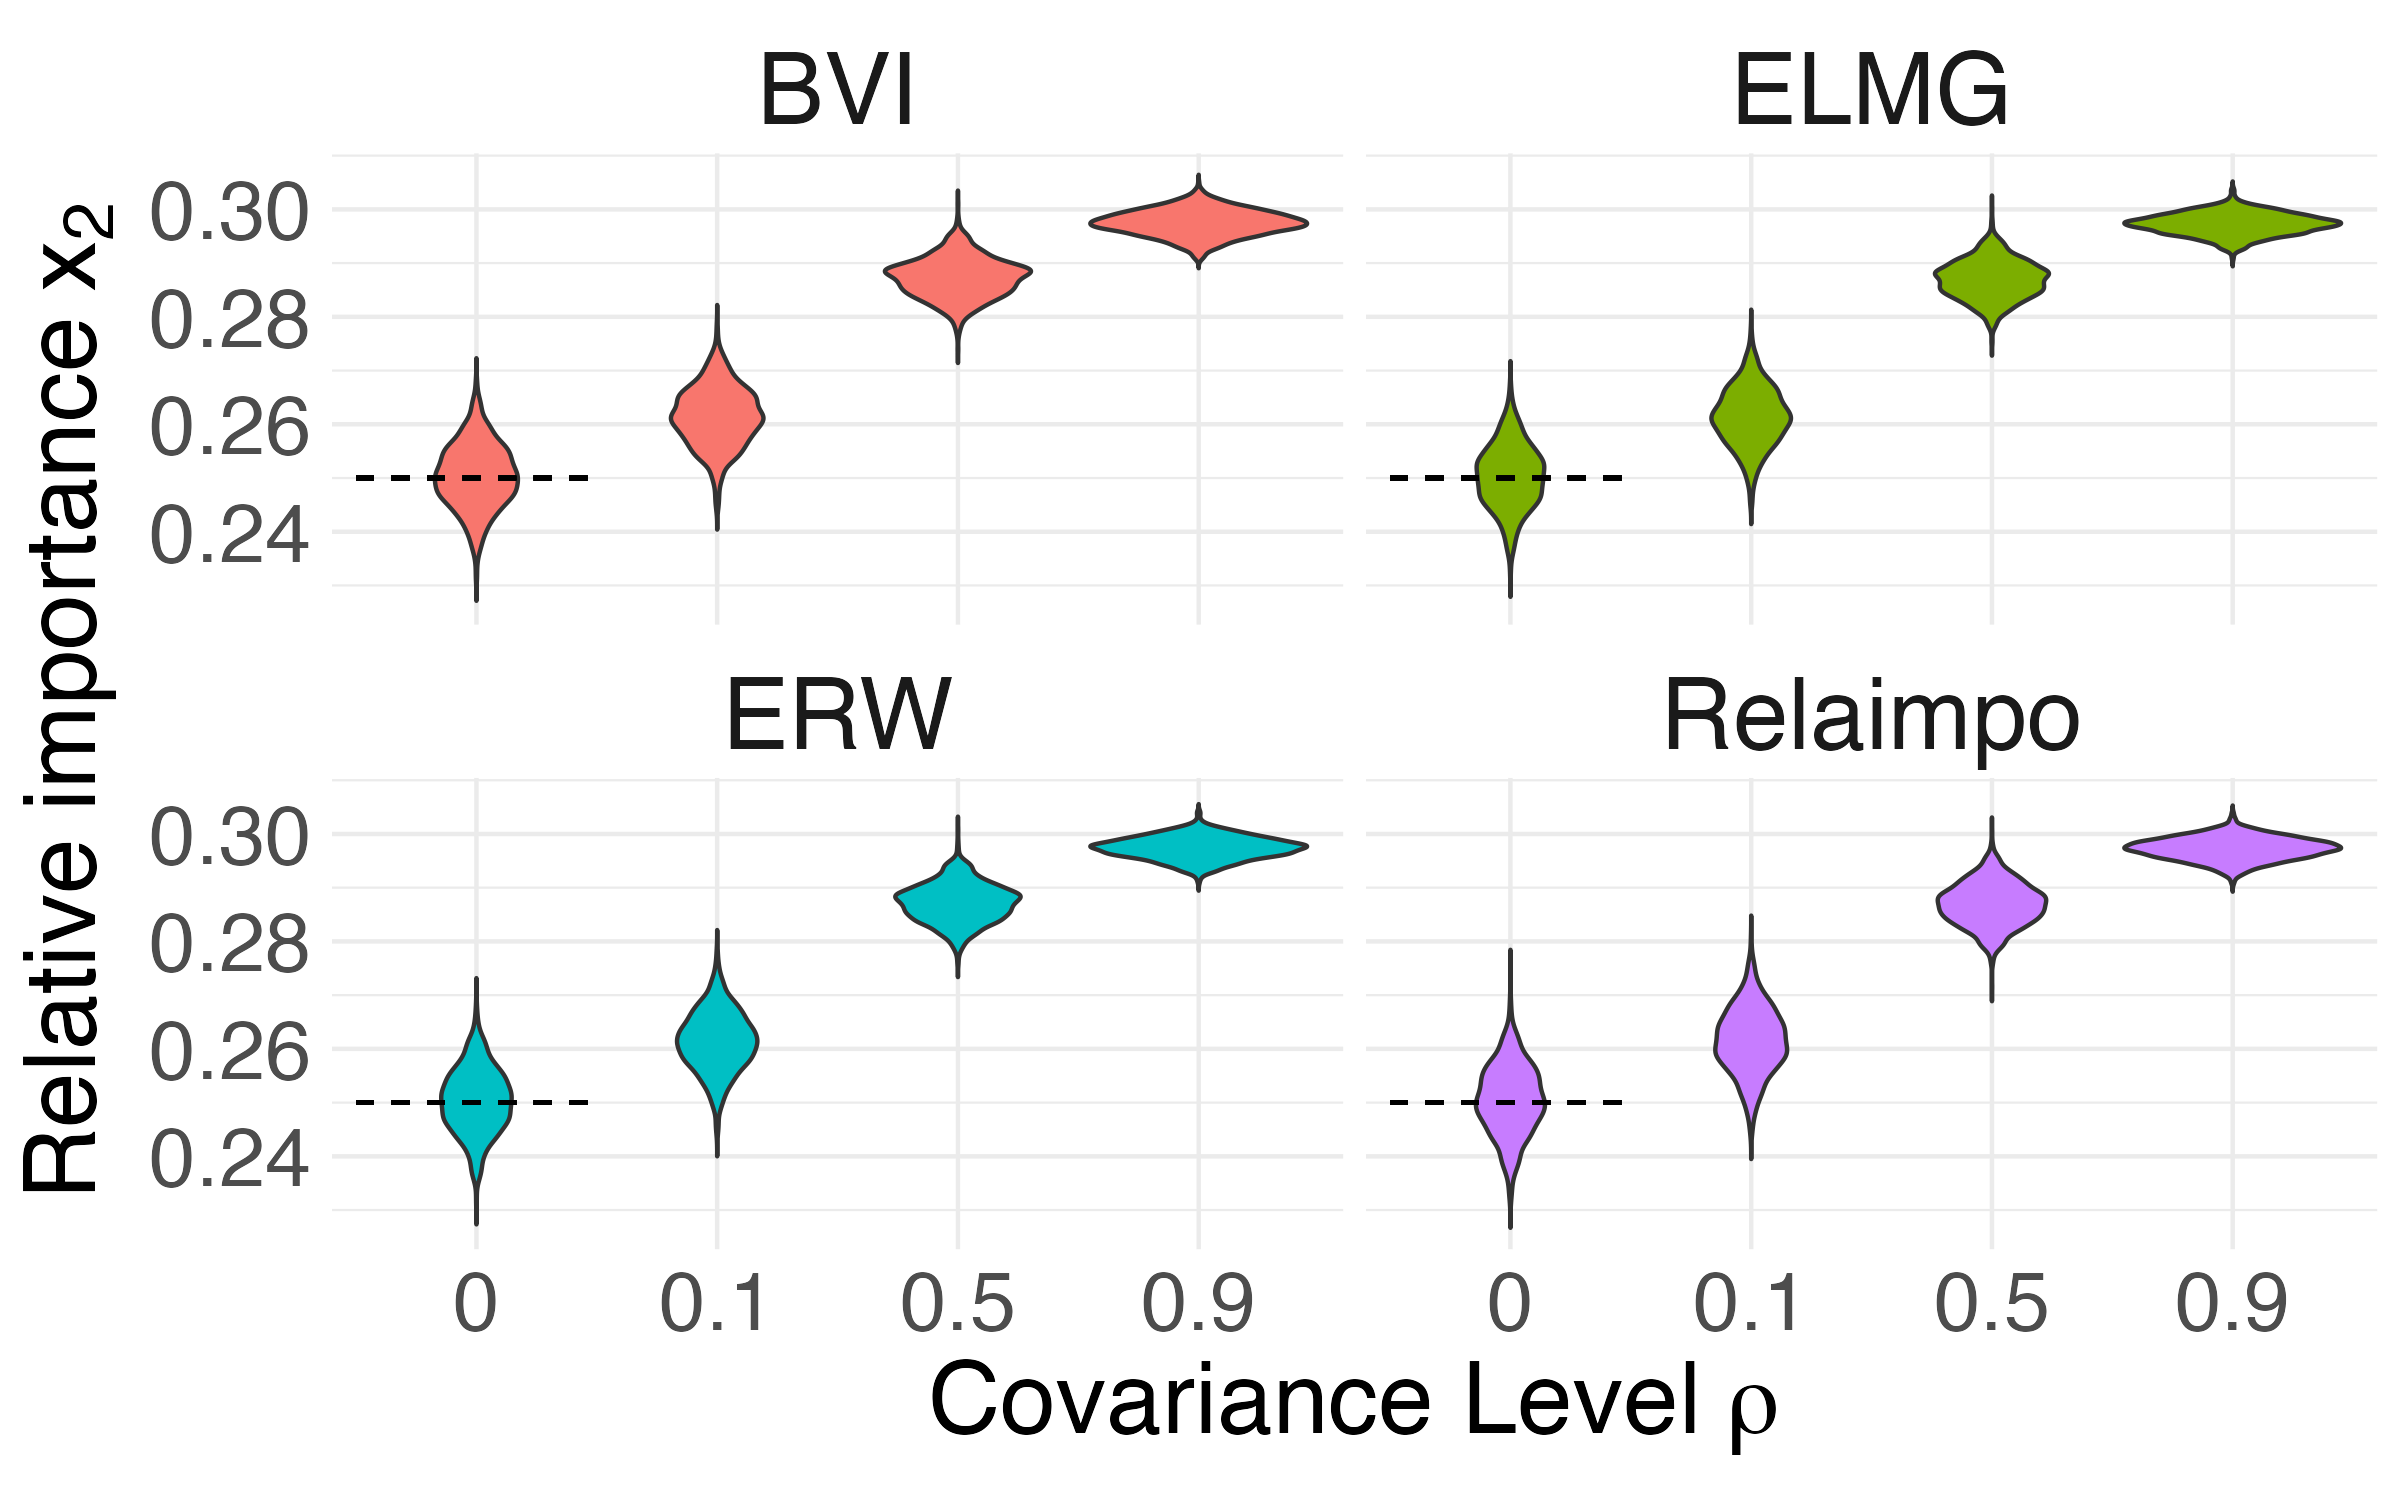
\includegraphics[width=0.7\linewidth]{Figures/ViolinPlots/Variance_V2.png}
    \caption{(b) Relative importance of $X_2$ as calculated from the four methods.}
    \label{fig:relimp_X2}
\end{figure}
\begin{figure}[H]\ContinuedFloat
  \centering
    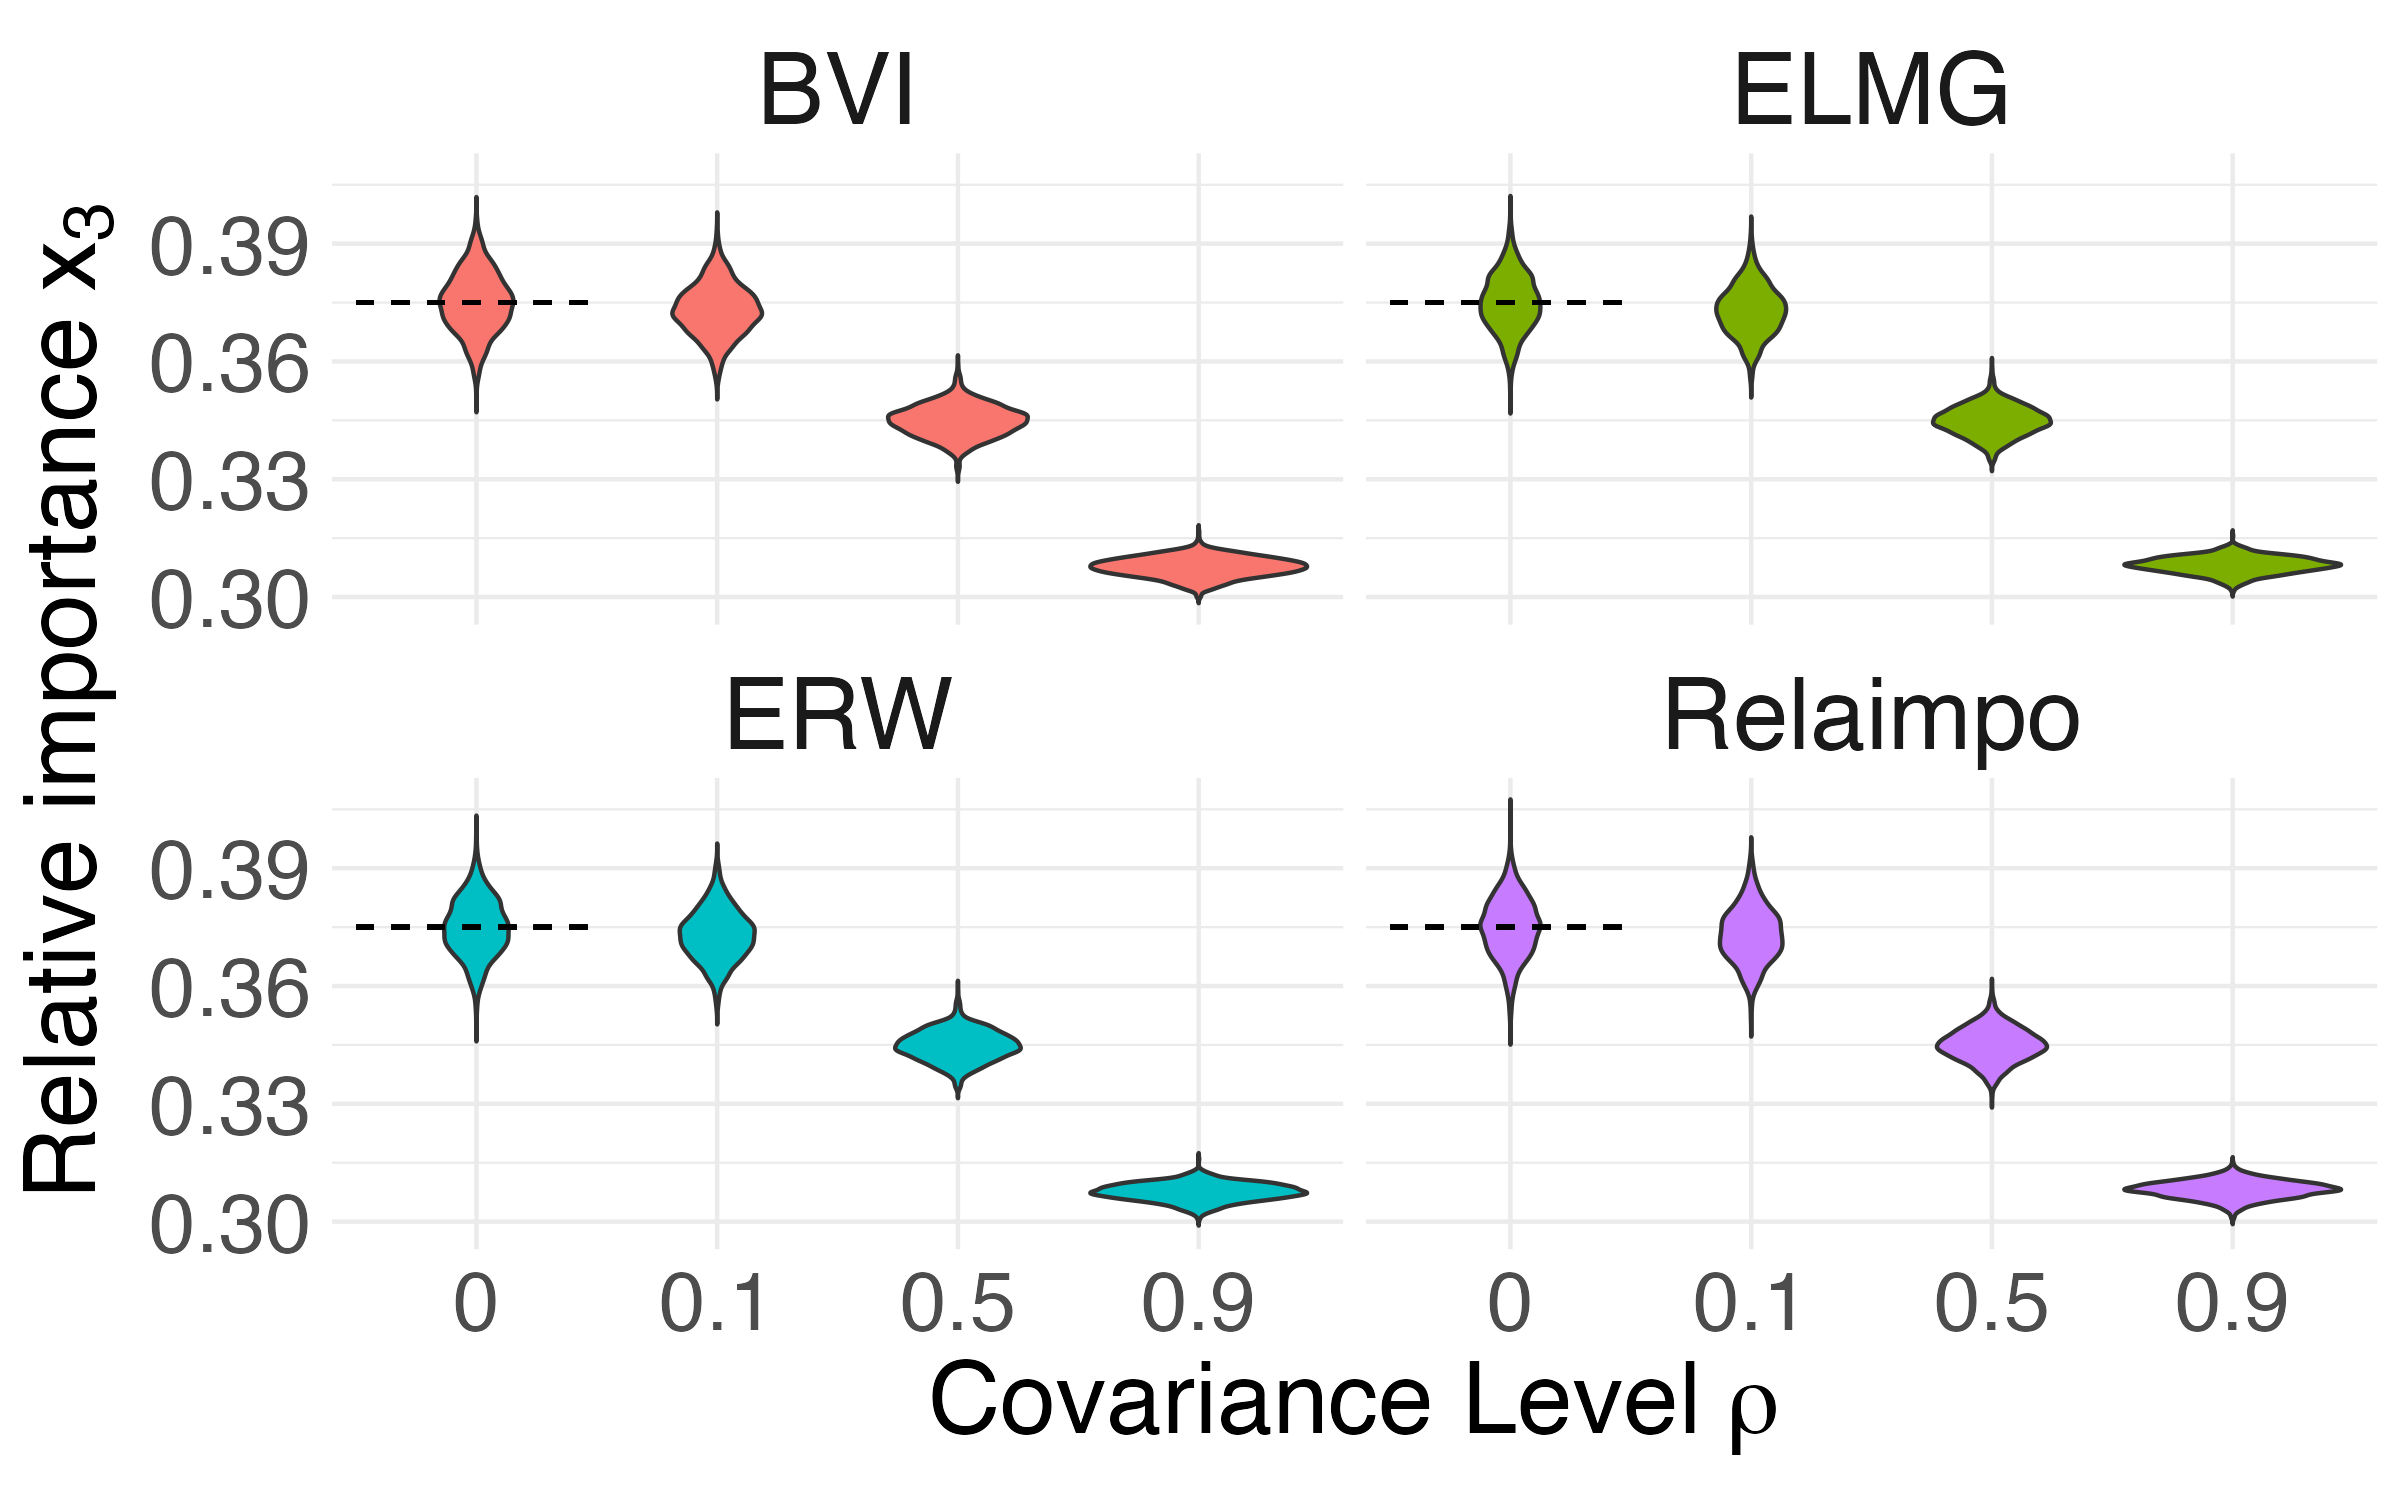
\includegraphics[width=0.7\linewidth]{Figures/ViolinPlots/Variance_V3.png}
    \caption{(c) Relative importance of $X_3$ as calculated from the four methods.}
    \label{fig:relimp_X3}
\end{figure}


% \begin{figure}[H]
%   \centering
%   \subfloat[Relative importance of $X_1$ as calculated from the four methods.]{
%     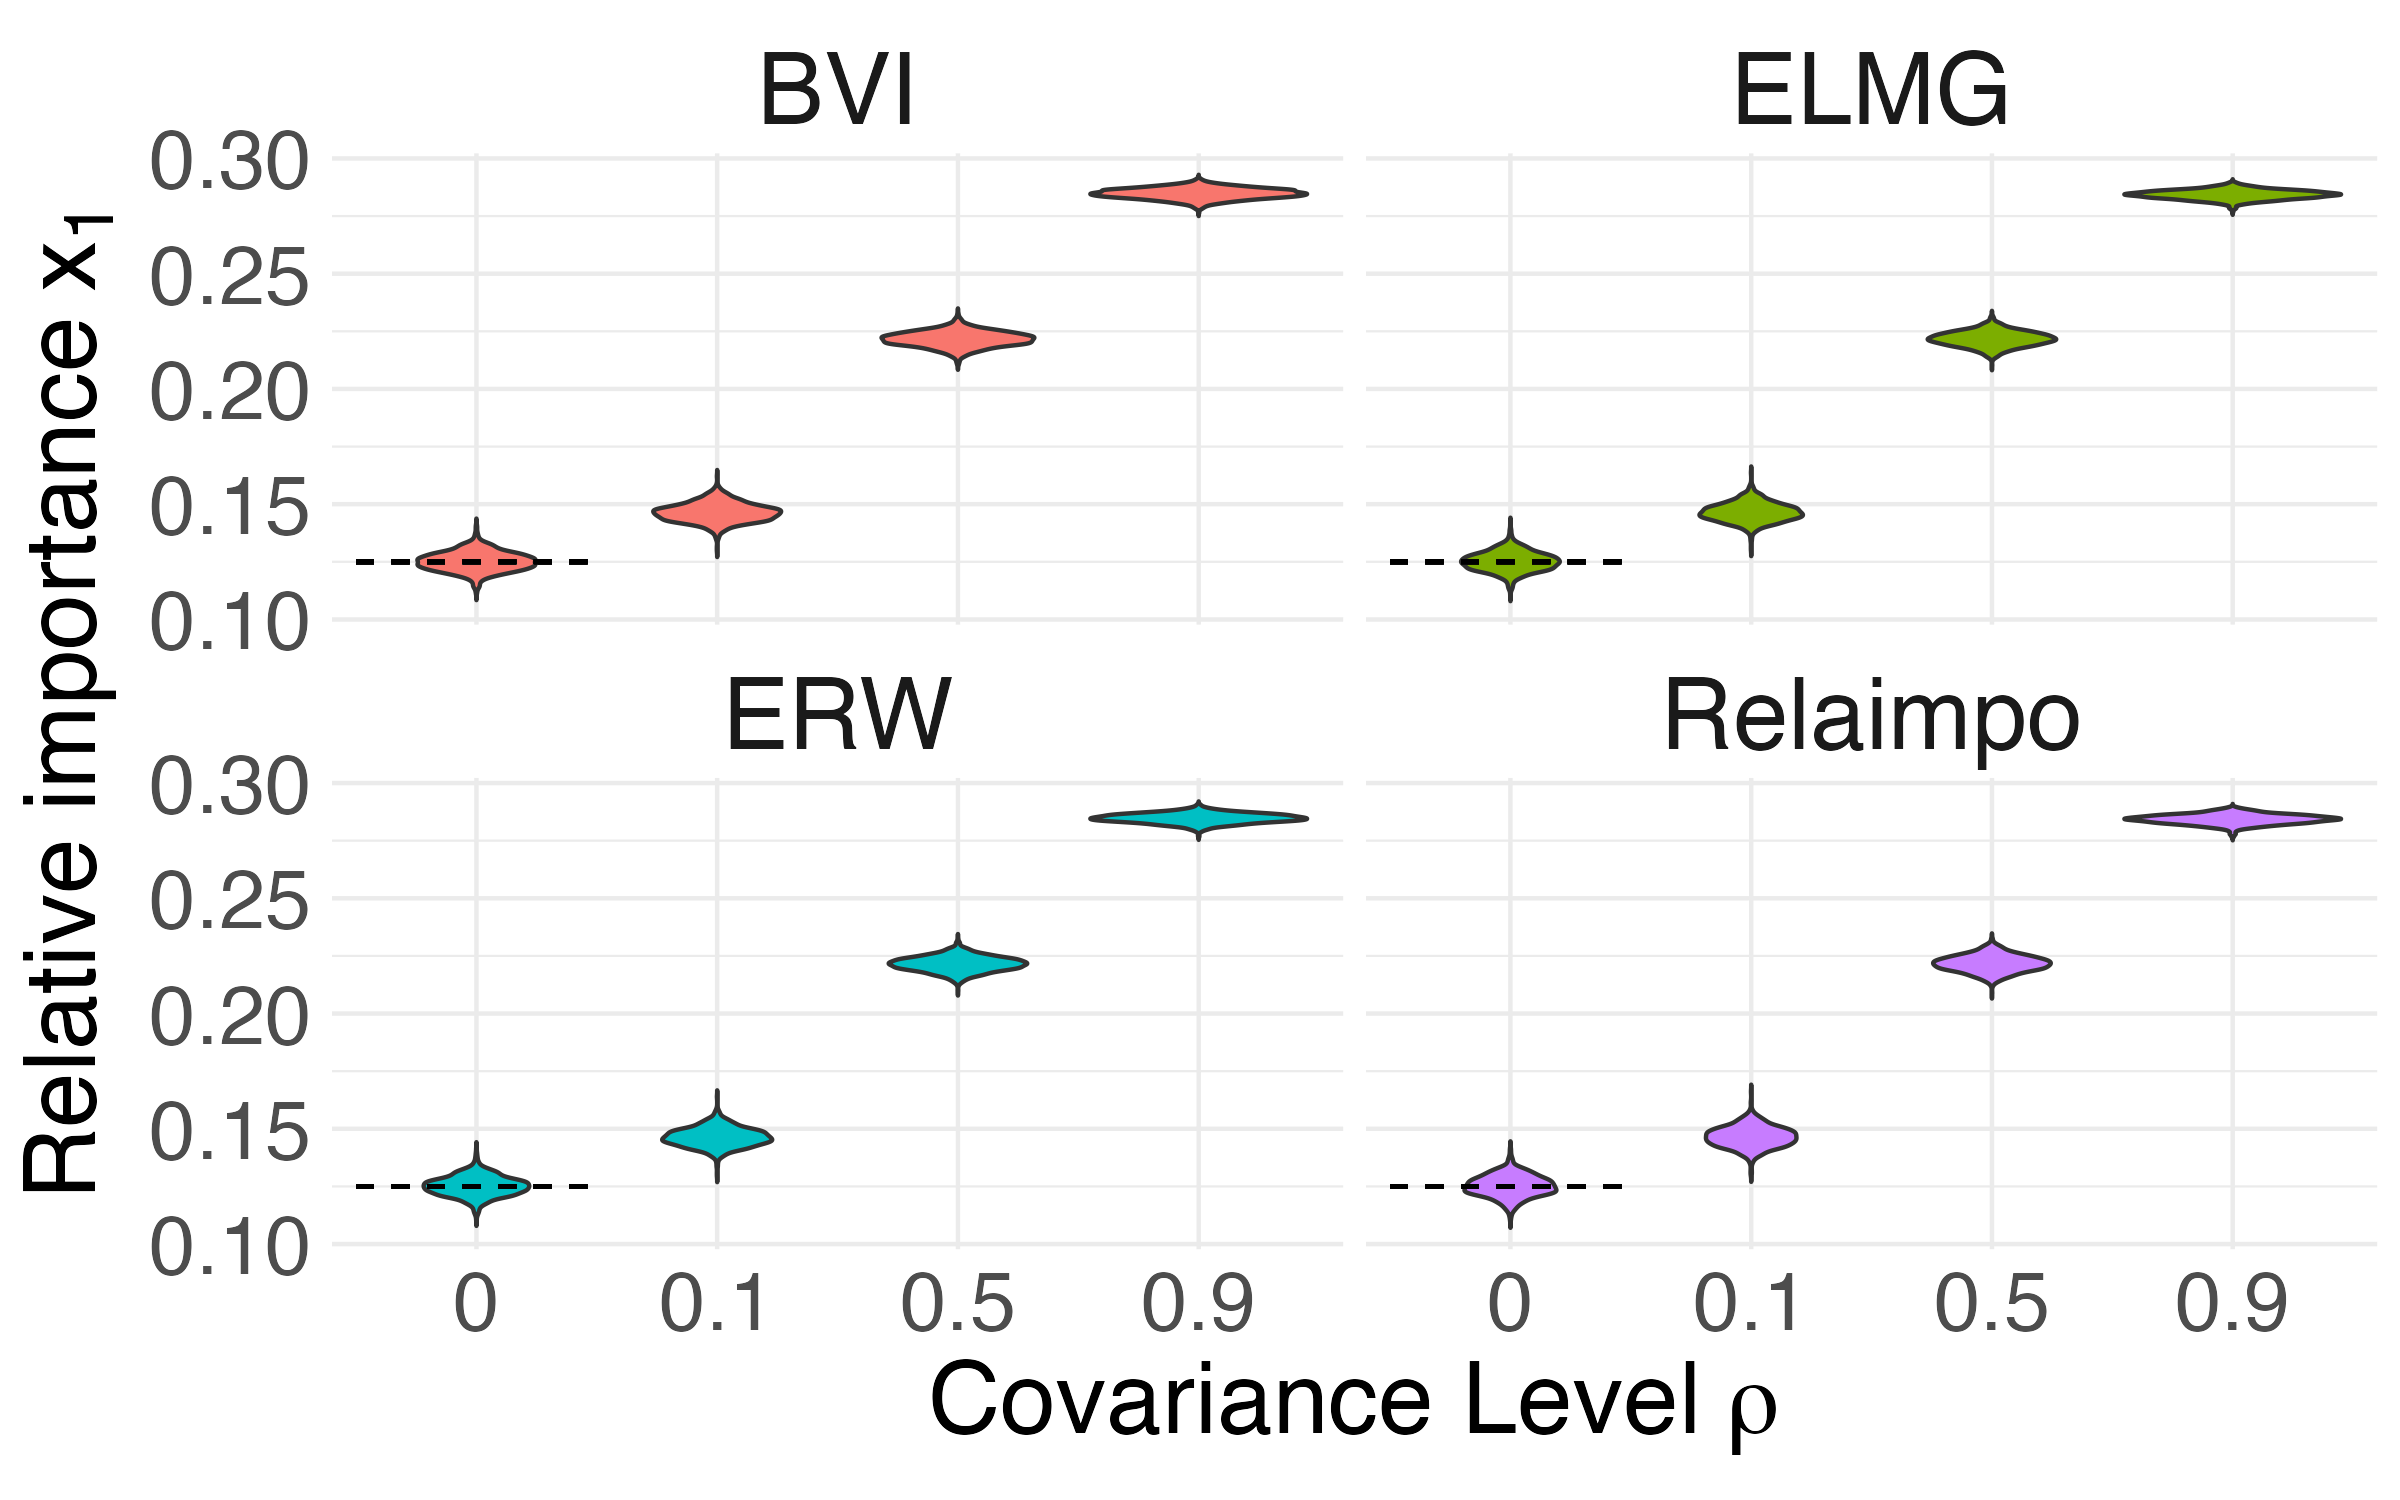
\includegraphics[width=0.6\linewidth]{Figures/ViolinPlots/Variance_V1.png}
%     \label{fig:relimp_X1}
%   }
%   \hfill
%   \subfloat[Relative importance of $X_2$ as calculated from the four methods.]{
%     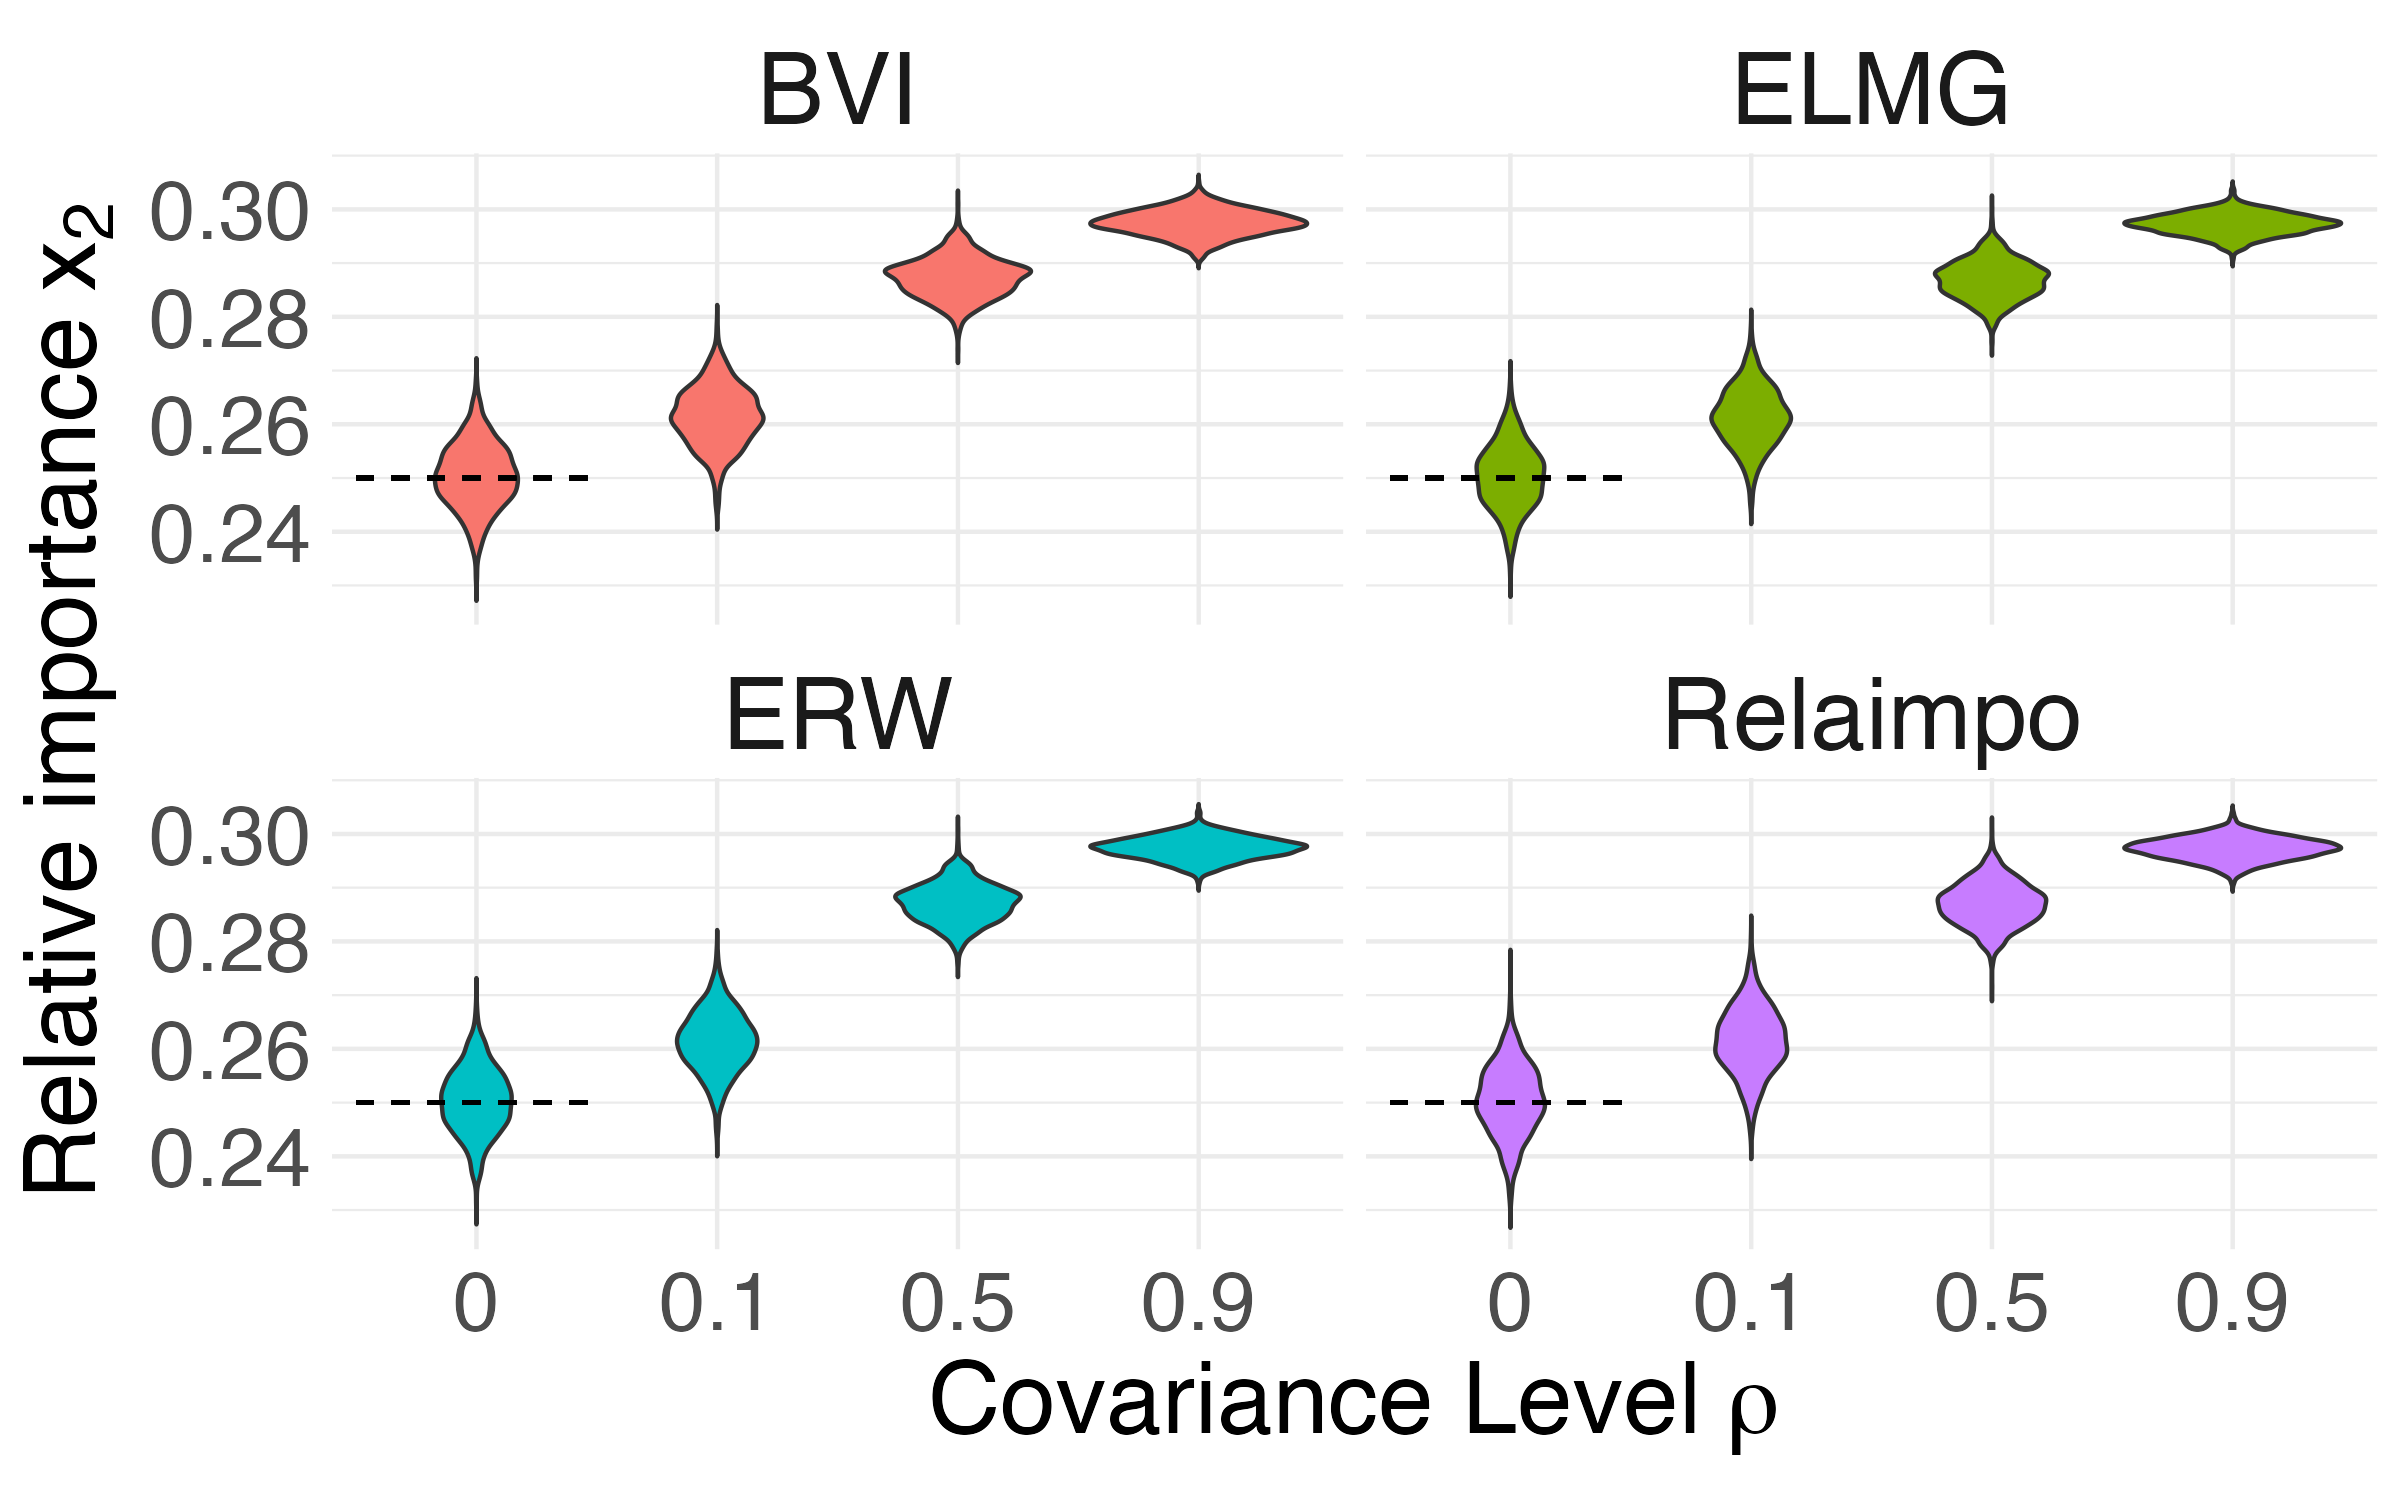
\includegraphics[width=0.6\linewidth]{Figures/ViolinPlots/Variance_V2.png}
%     \label{fig:relimp_X2}
%   }
%   \hfill
%   \subfloat[Relative importance of $X_3$ as calculated from the four methods.]{
%     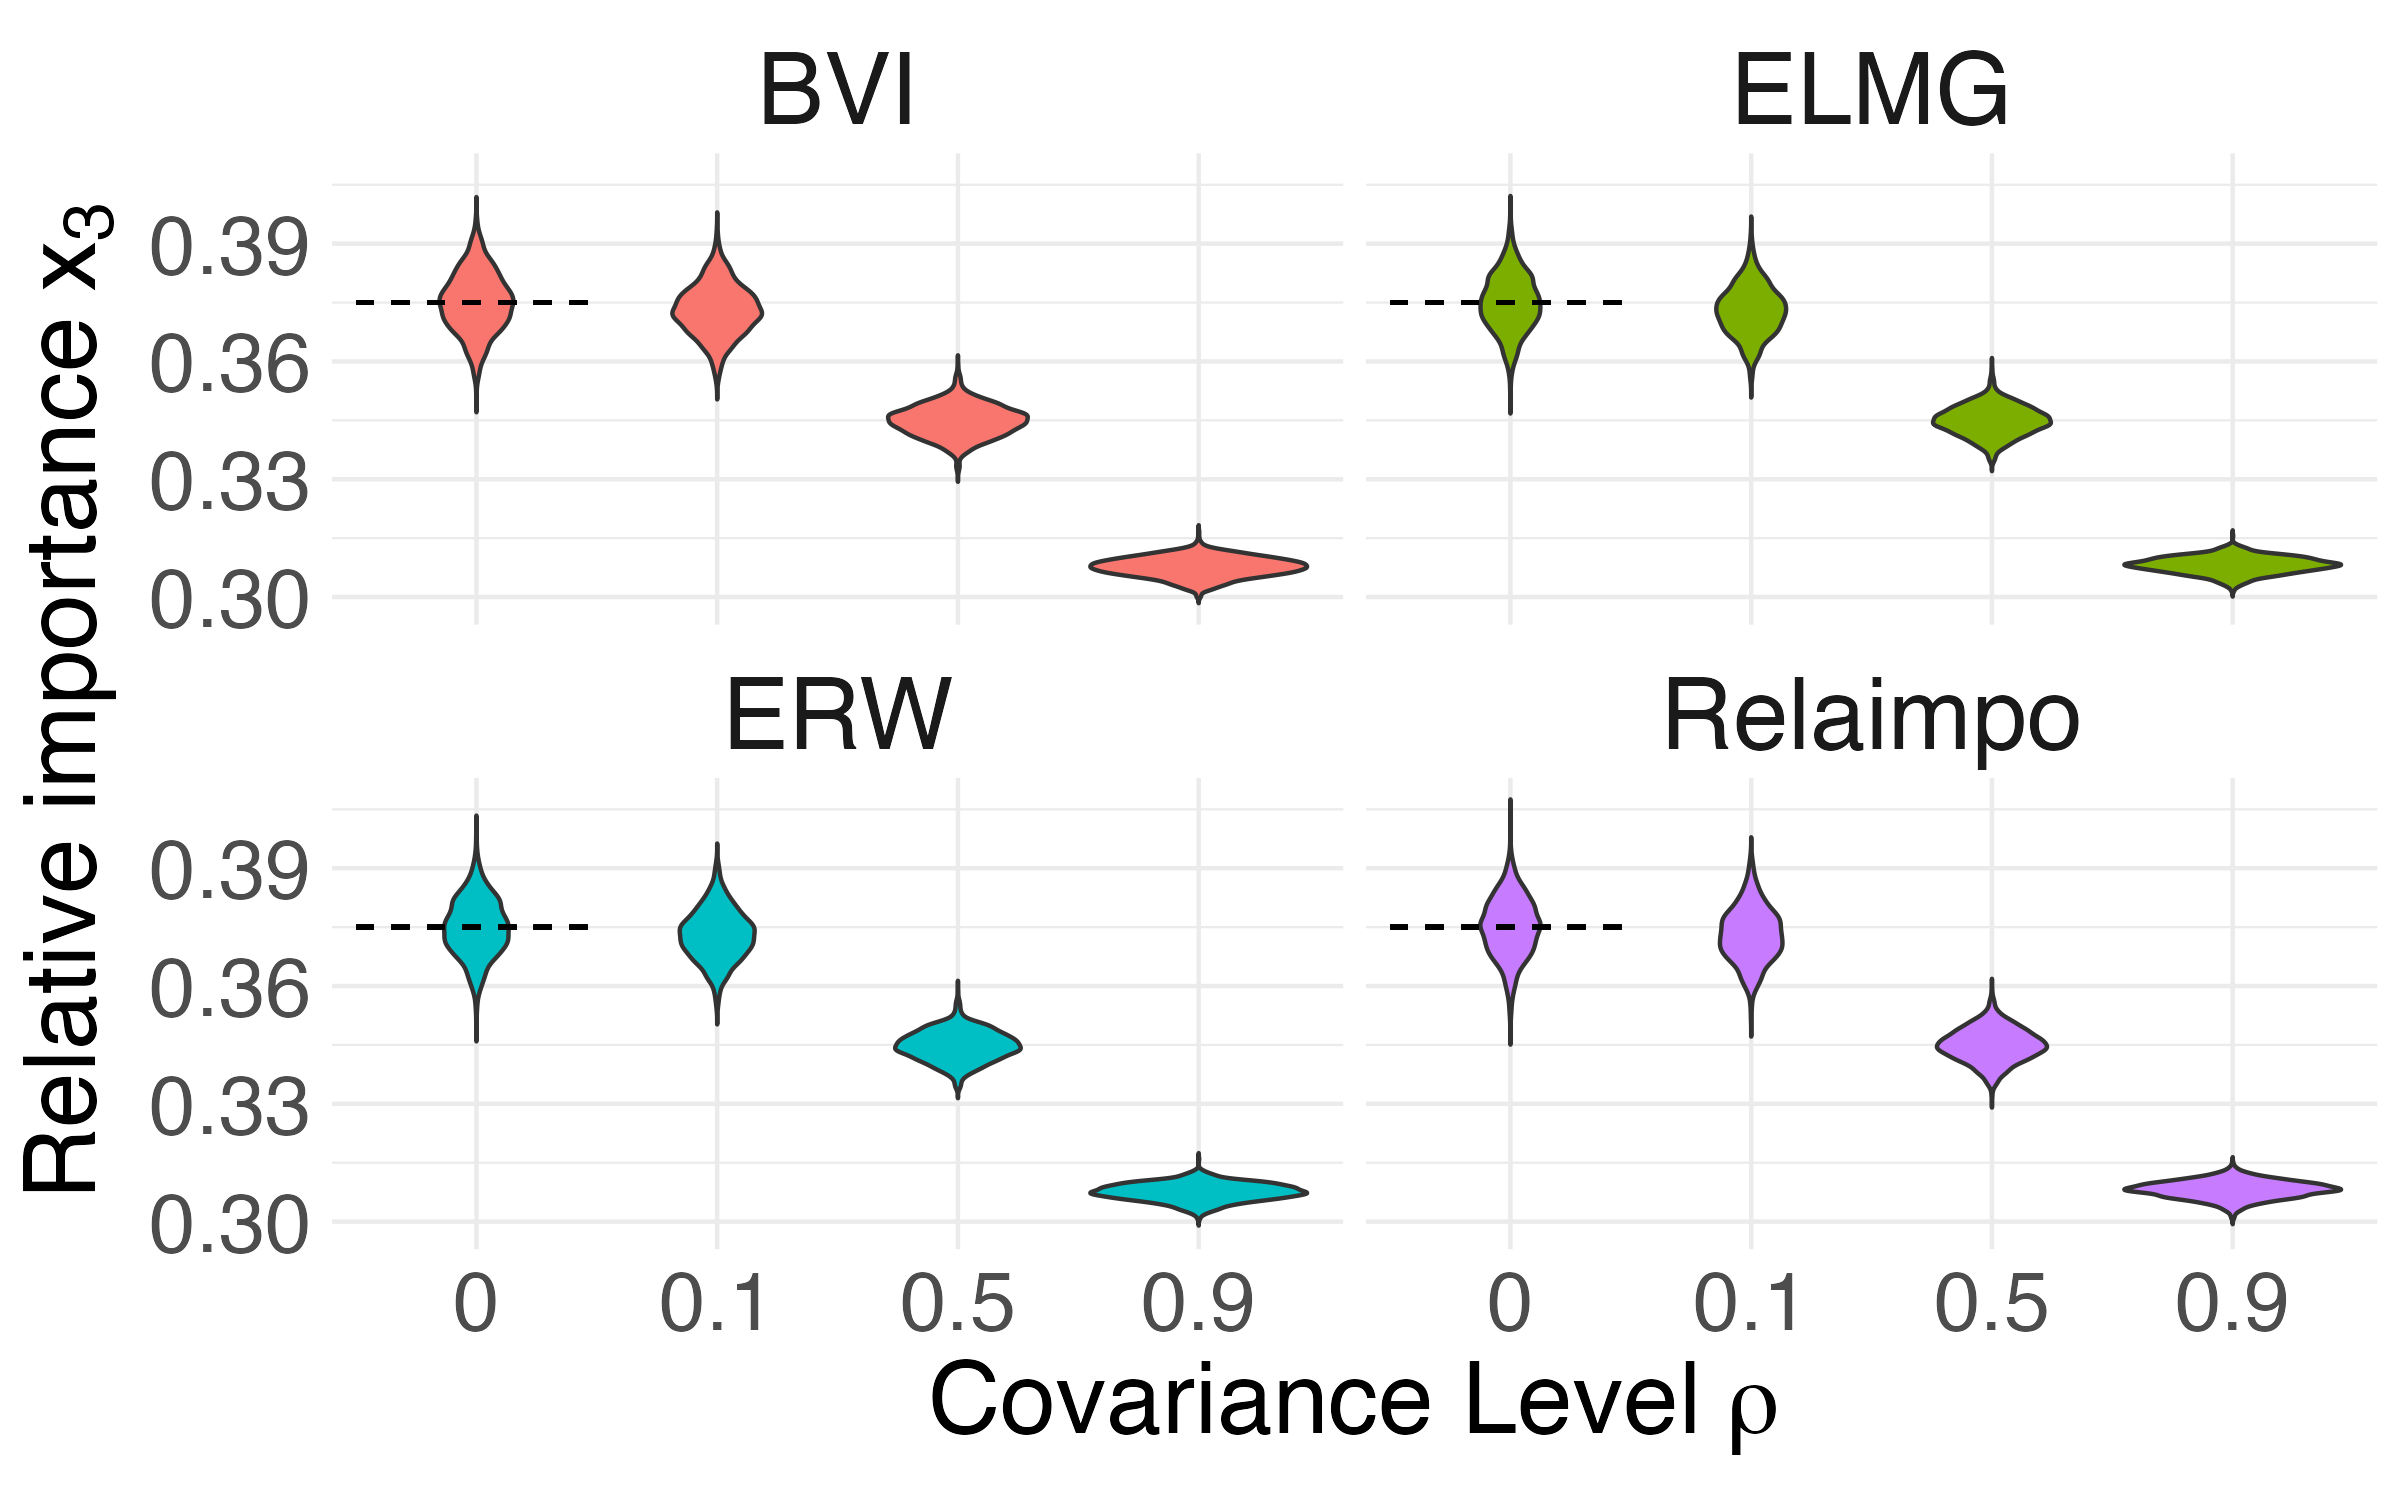
\includegraphics[width=0.6\linewidth]{Figures/ViolinPlots/Variance_V3.png}
%     \label{fig:relimp_X3}
%   }
%   \caption{Violin plots for the relative importance of the fixed effects $X_1, X_2$ and $X_3$ for different correlation levels calculated from $4\cdot 10^4$ simulated datasets by the BVI, ELMG, ERW and the Relaimpo method. The true, standardized regressor coefficients are $\boldsymbol{\beta}=\left(\sqrt{1/8}, \sqrt{2/8}, \sqrt{3/8}\right)$, and the true total model variance is $\sigma^2_{\mathbf{y}}=1$. For the BVI method the posterior means in each simulation are used to compare to the point estimates of the other three methods. The horizontal line displays the theoretically correct importance of each fixed effect in the case of uncorrelated data.}
%   \label{fig:relimp_fixed}
% \end{figure}


% We have, since $\boldsymbol{\Lambda}$ is symmetric, the importances
% \begin{equation} 
%   \begin{aligned}
%     \text{RI}(X_1) &= \boldsymbol{\Lambda}_{1, 1}^{[2]}\beta^{[2]}_1 + \boldsymbol{\Lambda}_{2, 1}^{[2]}\beta^{[2]}_2 + \boldsymbol{\Lambda}_{3, 1}^{[2]}\beta^{[2]}_3 \\ 
%     \text{RI}(X_2) &= \boldsymbol{\Lambda}_{2, 1}^{[2]}\beta^{[2]}_1 + \boldsymbol{\Lambda}_{2, 2}^{[2]}\beta^{[2]}_2 + \boldsymbol{\Lambda}_{3, 2}^{[2]}\beta^{[2]}_3 \\
%     \text{RI}(X_3) &= \boldsymbol{\Lambda}_{3, 1}^{[2]}\beta^{[2]}_1 + \boldsymbol{\Lambda}_{3, 2}^{[2]}\beta^{[2]}_2 + \boldsymbol{\Lambda}_{3, 3}^{[2]}\beta^{[2]}_3 \ ,
%   \end{aligned}
% \end{equation}
% where the columns of $\boldsymbol{\Lambda}^{[2]}$ sum to one. Clearly, if the of diagonal elements increase and the diagonal elements decrease, the importance  


% \begin{table}[!htb]
%   \centering
%   \caption{Your overall caption for all tables.}
%   \label{tab:your-overall-label}
  
%   % First row of tables
%   \begin{minipage}{.45\linewidth}
%   \centering
%   {\footnotesize
%   % latex table generated in R 4.2.1 by xtable 1.8-4 package
% Thu Dec 14 12:52:54 2023
\begin{table}[ht]
\centering
\begin{tabular}{lrrr}
  \hline
Method & Mean & Quantile\_2.5 & Quantile\_97.5 \\ 
  \hline
Relaimpo & 0.284272 & 0.280282 & 0.288313 \\ 
  BVI & 0.284761 & 0.280127 & 0.289150 \\ 
  ELMG & 0.284266 & 0.280411 & 0.288118 \\ 
  ERW & 0.284681 & 0.280541 & 0.288583 \\ 
   \hline
\end{tabular}
\end{table}

%   }
%   \end{minipage}%
%   \hfill
%   \begin{minipage}{.45\linewidth}
%   \centering
%   {\footnotesize
%   % latex table generated in R 4.2.1 by xtable 1.8-4 package
% Thu Dec 14 12:52:54 2023
\begin{table}[ht]
\centering
\begin{tabular}{lrrr}
  \hline
Method & Mean & Quantile\_2.5 & Quantile\_97.5 \\ 
  \hline
Relaimpo & 0.297261 & 0.293124 & 0.301180 \\ 
  BVI & 0.297466 & 0.292623 & 0.302066 \\ 
  ELMG & 0.297251 & 0.293040 & 0.300979 \\ 
  ERW & 0.297389 & 0.293189 & 0.301267 \\ 
   \hline
\end{tabular}
\end{table}

%   }
%   \end{minipage}
  
%   \vspace{5mm} % Adjust the vertical space as needed
  
%   % Second row of tables
%   \begin{minipage}{.45\linewidth}
%   \centering
%   {\footnotesize
%   % latex table generated in R 4.2.1 by xtable 1.8-4 package
% Thu Dec 14 12:52:54 2023
\begin{table}[ht]
\centering
\begin{tabular}{lrrr}
  \hline
Method & Mean & Quantile\_2.5 & Quantile\_97.5 \\ 
  \hline
Relaimpo & 0.308142 & 0.303571 & 0.312266 \\ 
  BVI & 0.307594 & 0.302328 & 0.312071 \\ 
  ELMG & 0.308110 & 0.303704 & 0.312229 \\ 
  ERW & 0.307534 & 0.302991 & 0.311786 \\ 
   \hline
\end{tabular}
\end{table}

%   }
%   \end{minipage}%
%   \hfill
%   \begin{minipage}{.45\linewidth}
%   \centering
%   {\footnotesize
%   % latex table generated in R 4.2.1 by xtable 1.8-4 package
% Thu Dec 14 12:52:54 2023
\begin{table}[ht]
\centering
\begin{tabular}{lrrr}
  \hline
Method & Mean & Quantile\_2.5 & Quantile\_97.5 \\ 
  \hline
Relaimpo &  &  &  \\ 
  BVI & 0.055443 & 0.046108 & 0.066800 \\ 
  ELMG & 0.055070 & 0.045624 & 0.066502 \\ 
  ERW & 0.055094 & 0.044524 & 0.067235 \\ 
   \hline
\end{tabular}
\end{table}

%   }
%   \end{minipage}
  
% \end{table}
  
  
% \end{table}
% % latex table generated in R 4.2.1 by xtable 1.8-4 package
% Thu Dec 14 12:52:54 2023
\begin{table}[ht]
\centering
\begin{tabular}{lrrr}
  \hline
Method & Mean & Quantile\_2.5 & Quantile\_97.5 \\ 
  \hline
Relaimpo & 0.284272 & 0.280282 & 0.288313 \\ 
  BVI & 0.284761 & 0.280127 & 0.289150 \\ 
  ELMG & 0.284266 & 0.280411 & 0.288118 \\ 
  ERW & 0.284681 & 0.280541 & 0.288583 \\ 
   \hline
\end{tabular}
\end{table}

% % latex table generated in R 4.2.1 by xtable 1.8-4 package
% Thu Dec 14 12:52:54 2023
\begin{table}[ht]
\centering
\begin{tabular}{lrrr}
  \hline
Method & Mean & Quantile\_2.5 & Quantile\_97.5 \\ 
  \hline
Relaimpo & 0.297261 & 0.293124 & 0.301180 \\ 
  BVI & 0.297466 & 0.292623 & 0.302066 \\ 
  ELMG & 0.297251 & 0.293040 & 0.300979 \\ 
  ERW & 0.297389 & 0.293189 & 0.301267 \\ 
   \hline
\end{tabular}
\end{table}

% % latex table generated in R 4.2.1 by xtable 1.8-4 package
% Thu Dec 14 12:52:54 2023
\begin{table}[ht]
\centering
\begin{tabular}{lrrr}
  \hline
Method & Mean & Quantile\_2.5 & Quantile\_97.5 \\ 
  \hline
Relaimpo & 0.308142 & 0.303571 & 0.312266 \\ 
  BVI & 0.307594 & 0.302328 & 0.312071 \\ 
  ELMG & 0.308110 & 0.303704 & 0.312229 \\ 
  ERW & 0.307534 & 0.302991 & 0.311786 \\ 
   \hline
\end{tabular}
\end{table}

% Displayed in figure \ref{fig:relimp_fixed} are the calculated relative importances for the fixed effects for different covariance levels, along with the theoretically correct value when the data are uncorrelated as a dashed line. 
% %Rewrite the above sentence

% %Go thorugh each plot for the different regressors as below and discuss and compare all methods.
% For $X_1$ the relative importance is $\beta_1^2$ and we see in \ref{fig:relimp_X1} that all methods are consistent when the data are uncorrelated, giving a violin that is evenly distributed about the correct value $\frac{1}{8} = 0.125$.

%In general, our method produces results that are very similar to that of established methods for the fixed effects, and follows the same trends. 
%Should I make the limits of the plots tighter so that the violins become bigger? The problem then is that we lose the same axis.

\subsection{Relative importance of the random effects}
\label{sec:relimp_random}
Considering a model with one random intercept, we can no longer compare our model with the Relaimpo method, which is only implemented for the linear regression in the relaimpo R package \citep{gromping_relaimpo}. Therefore, we now compare the BVI method only with the ELMG and ERW methods, which have been extended from the Relaimpo method \citep{matre}.
\Cref{fig:relimp_alpha} shows the distribution of the relative importance, or variance, assigned to the random intercept $\boldsymbol{\alpha}$ for different correlation levels. 
The random intercept $\boldsymbol{\alpha}$ follows a univariate normal distribution with variance equal to $1/8$ and the standard deviation of the response is $\sigma^2_{\mathbf{y}}=1$. 
As before the horizontal line shows the theoretical relative importance that $\boldsymbol{\alpha}$ has in the model when the fixed effects are uncorrelated.
\newline
\newline
From \Cref{fig:relimp_alpha} it is apparent that both the location and width of the relative importance distribution of all methods are largely indistinguishable. 
The distributions take on a moderately smaller value when $\rho=0.1$ and the location of the estimates is further decreased for $\rho=0.5$ and $\rho=0.9$. 
For the latter correlation level, the distributions are located around a value that is less than half of the value of the centering when the fixed effects are uncorrelated. 
To re-emphasize, this is both expected and desirable since the increase in response variance comes solely from the correlation of fixed effects, so the random effects now contribute to explain a smaller proportion of the variance, \textit{i.e.} the importance is lower.
\begin{figure}[ht]
  \centering
  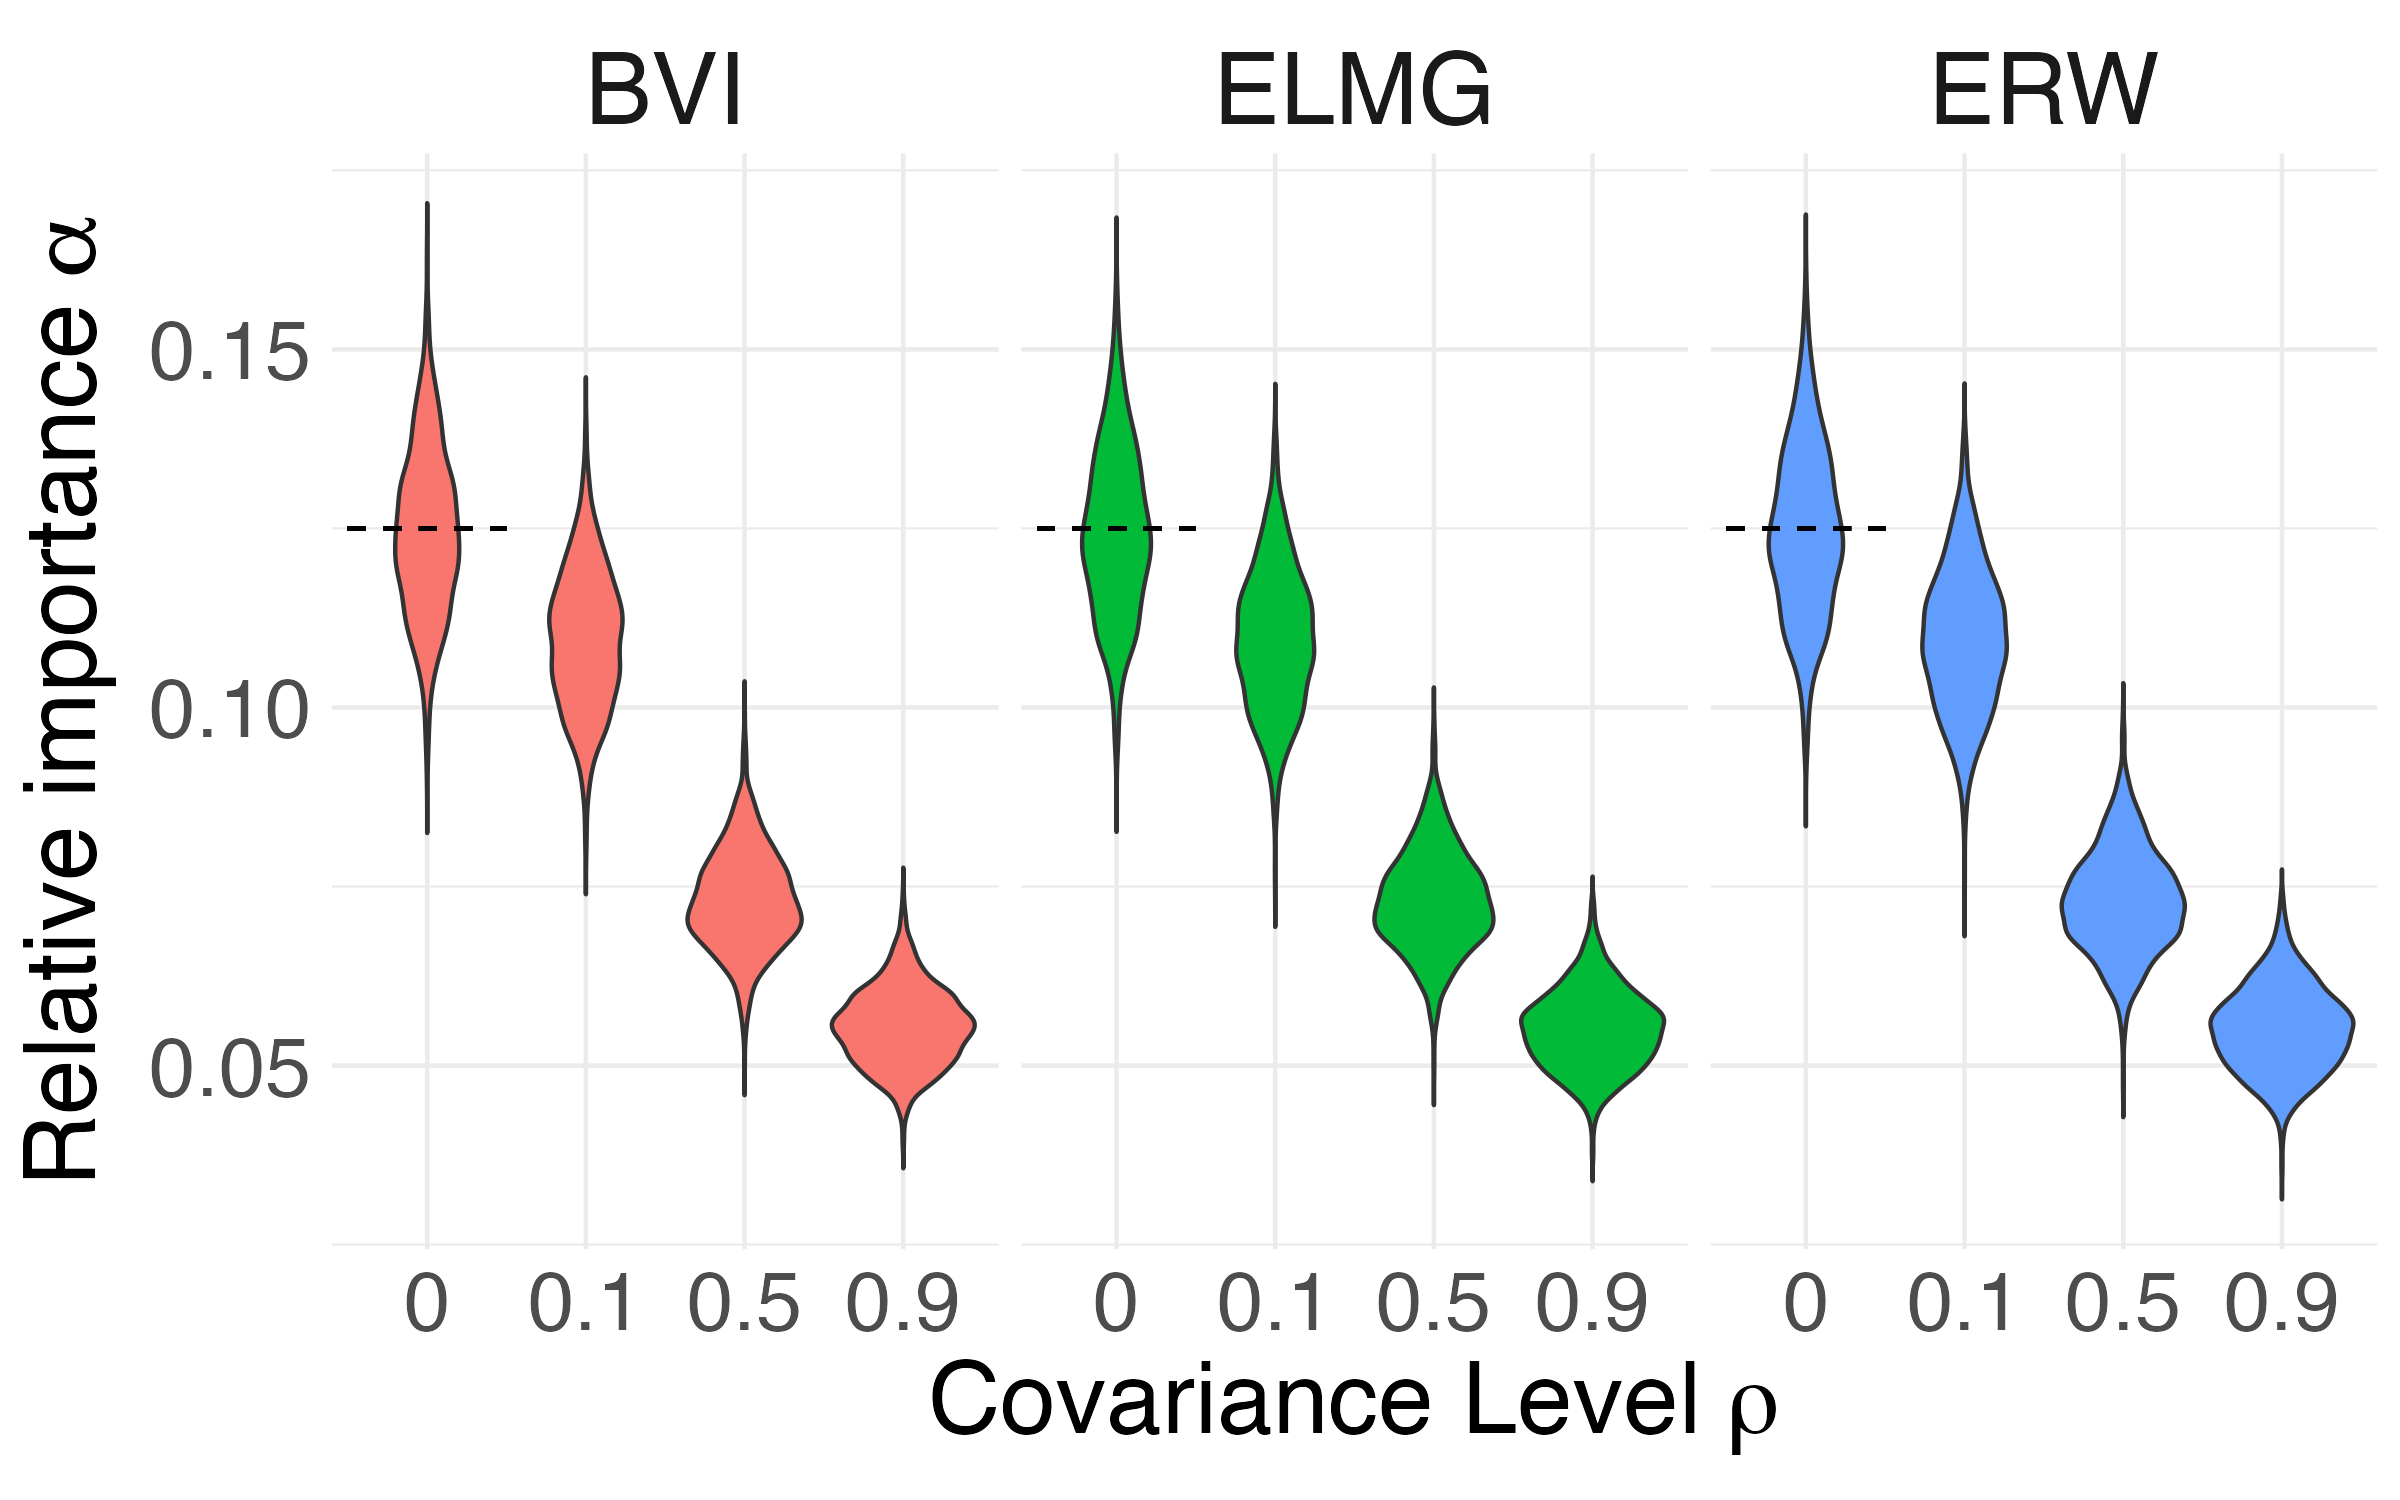
\includegraphics[width=0.7\linewidth]{Figures/ViolinPlots/Variance_gamma.png}
  \caption{Violin plots for the relative importance of the random effect $\boldsymbol{\alpha}$, that is, $\hat{\sigma}^2_{\alpha}$ for different correlation levels calculated from the ensemble of simulated datasets by the BVI, ELMG and the ERW method. For the BVI method the distributions of posterior means of the marginal distribution of $\hat{\sigma}^2_{\alpha}$ are shown to compare to the point estimates of the other two methods. The horizontal line displays the theoretically correct importance $\sigma^2_{\alpha} = 0.125$ of the random effect in the case of uncorrelated data.}
  \label{fig:relimp_alpha}
\end{figure}

\subsection{Total variance explained - $R^2$ estimates}
\label{sec:R2} 
As a useful by-product from the previous results we can get the total variances explained by our model (\Cref{fig:total_variance}).
The marginal variance explained is the variance explained by the fixed effects (\Cref{fig:variance_marginal}), and we get results for all four methods, including Relaimpo.
In \Cref{fig:variance_conditional} the total conditional variance explained, $R^2_{\text{cond}}$, is displayed. 
This is the variance given all the fixed effects and the random effect.
To complement the conditional and marginal variances explained, a horizontal line is drawn for each correlation level corresponding to the theoretically correct variance explained, found in \Cref{table:1}, for the correlation level. 
\newline
\newline
\Cref{fig:variance_marginal} shows that the four methods produce very similar results of $R^2_{\text{marg}}$ for the fixed effects across all correlation values, albeit a slightly larger width for the BVI method can be seen.
When considering the conditional variance $R^2_{\text{cond}}$ in \Cref{fig:variance_conditional}, the dispersion of the BVI method is strikingly larger compared to the other methods. 

Both the marginal and the conditional variance are centered around the theoretically correct value with some variability, particularly visible for conditional variance of the BVI method. 
The centering of the distributions for both the marginal and conditional variances resemble each other for all methods, regardless of correlation level.
\begin{figure}[!ht]
  \centering
  % First row
  \subfloat[Total marginal variance $R^2_{\text{marg}}$.]{
    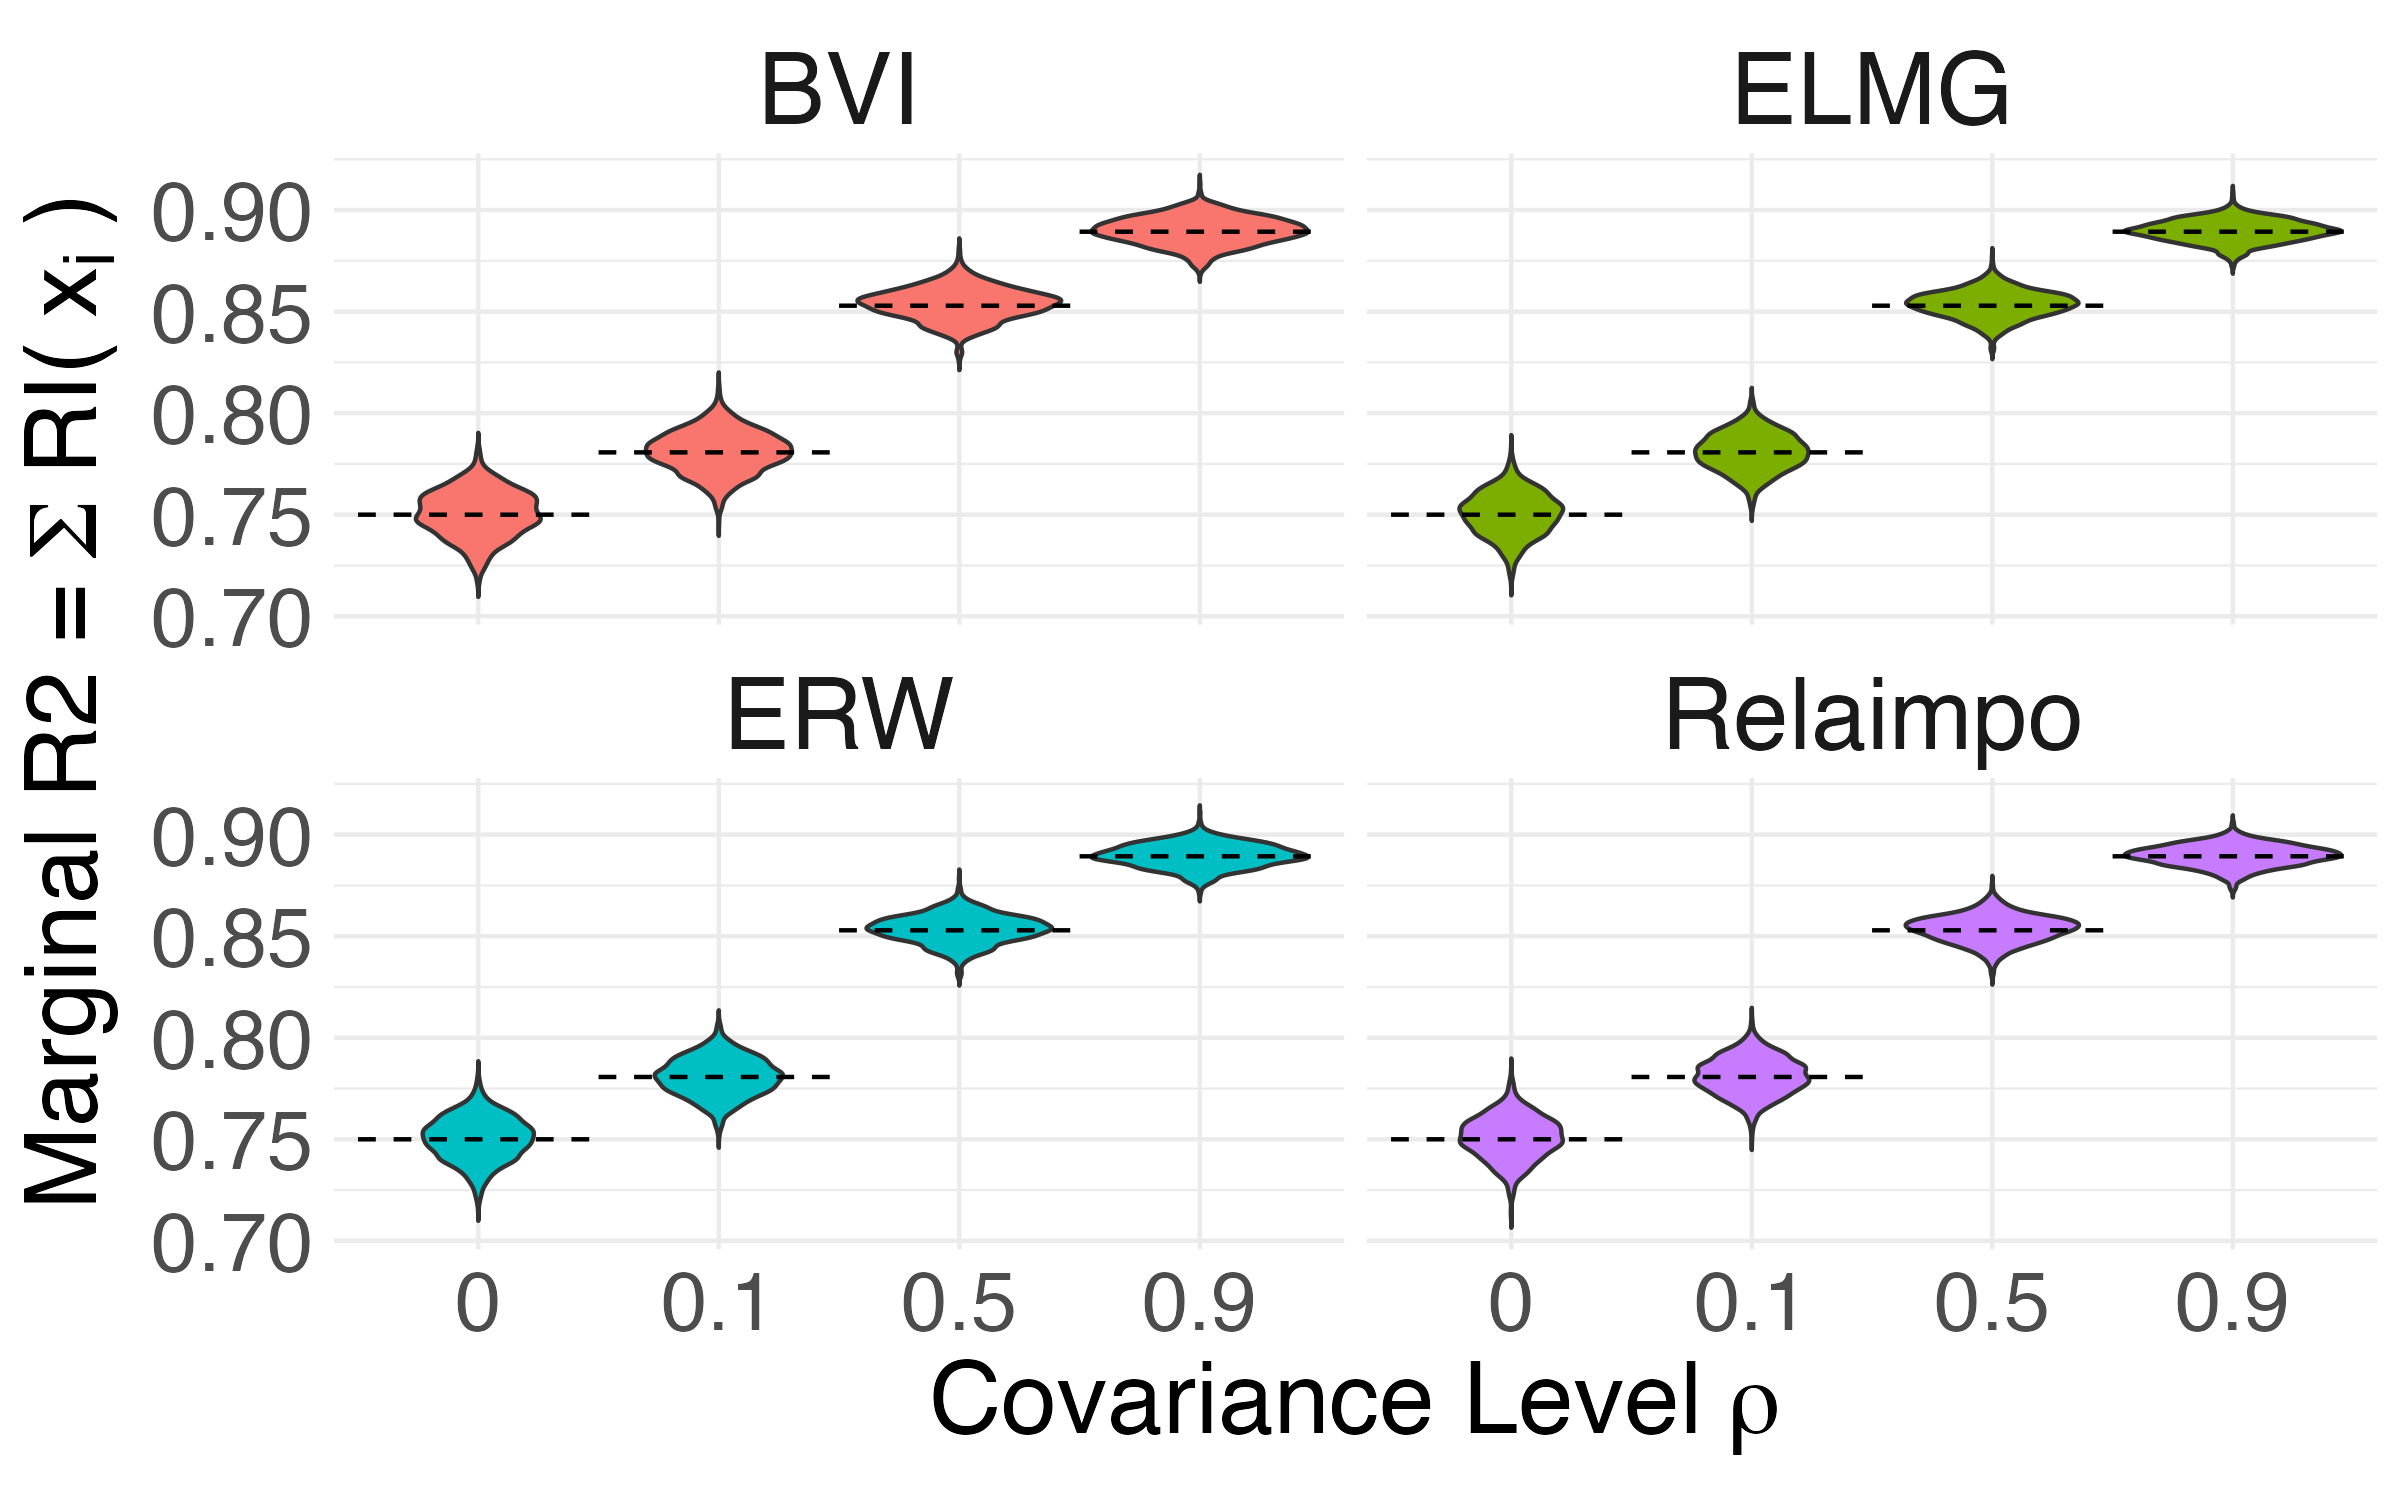
\includegraphics[width=0.6\linewidth]{Figures/ViolinPlots/Marginal_Variance.png}
    \label{fig:variance_marginal}
  }
  \hfill
  \subfloat[Total conditional variance $R^2_{\text{cond}}$.]{
    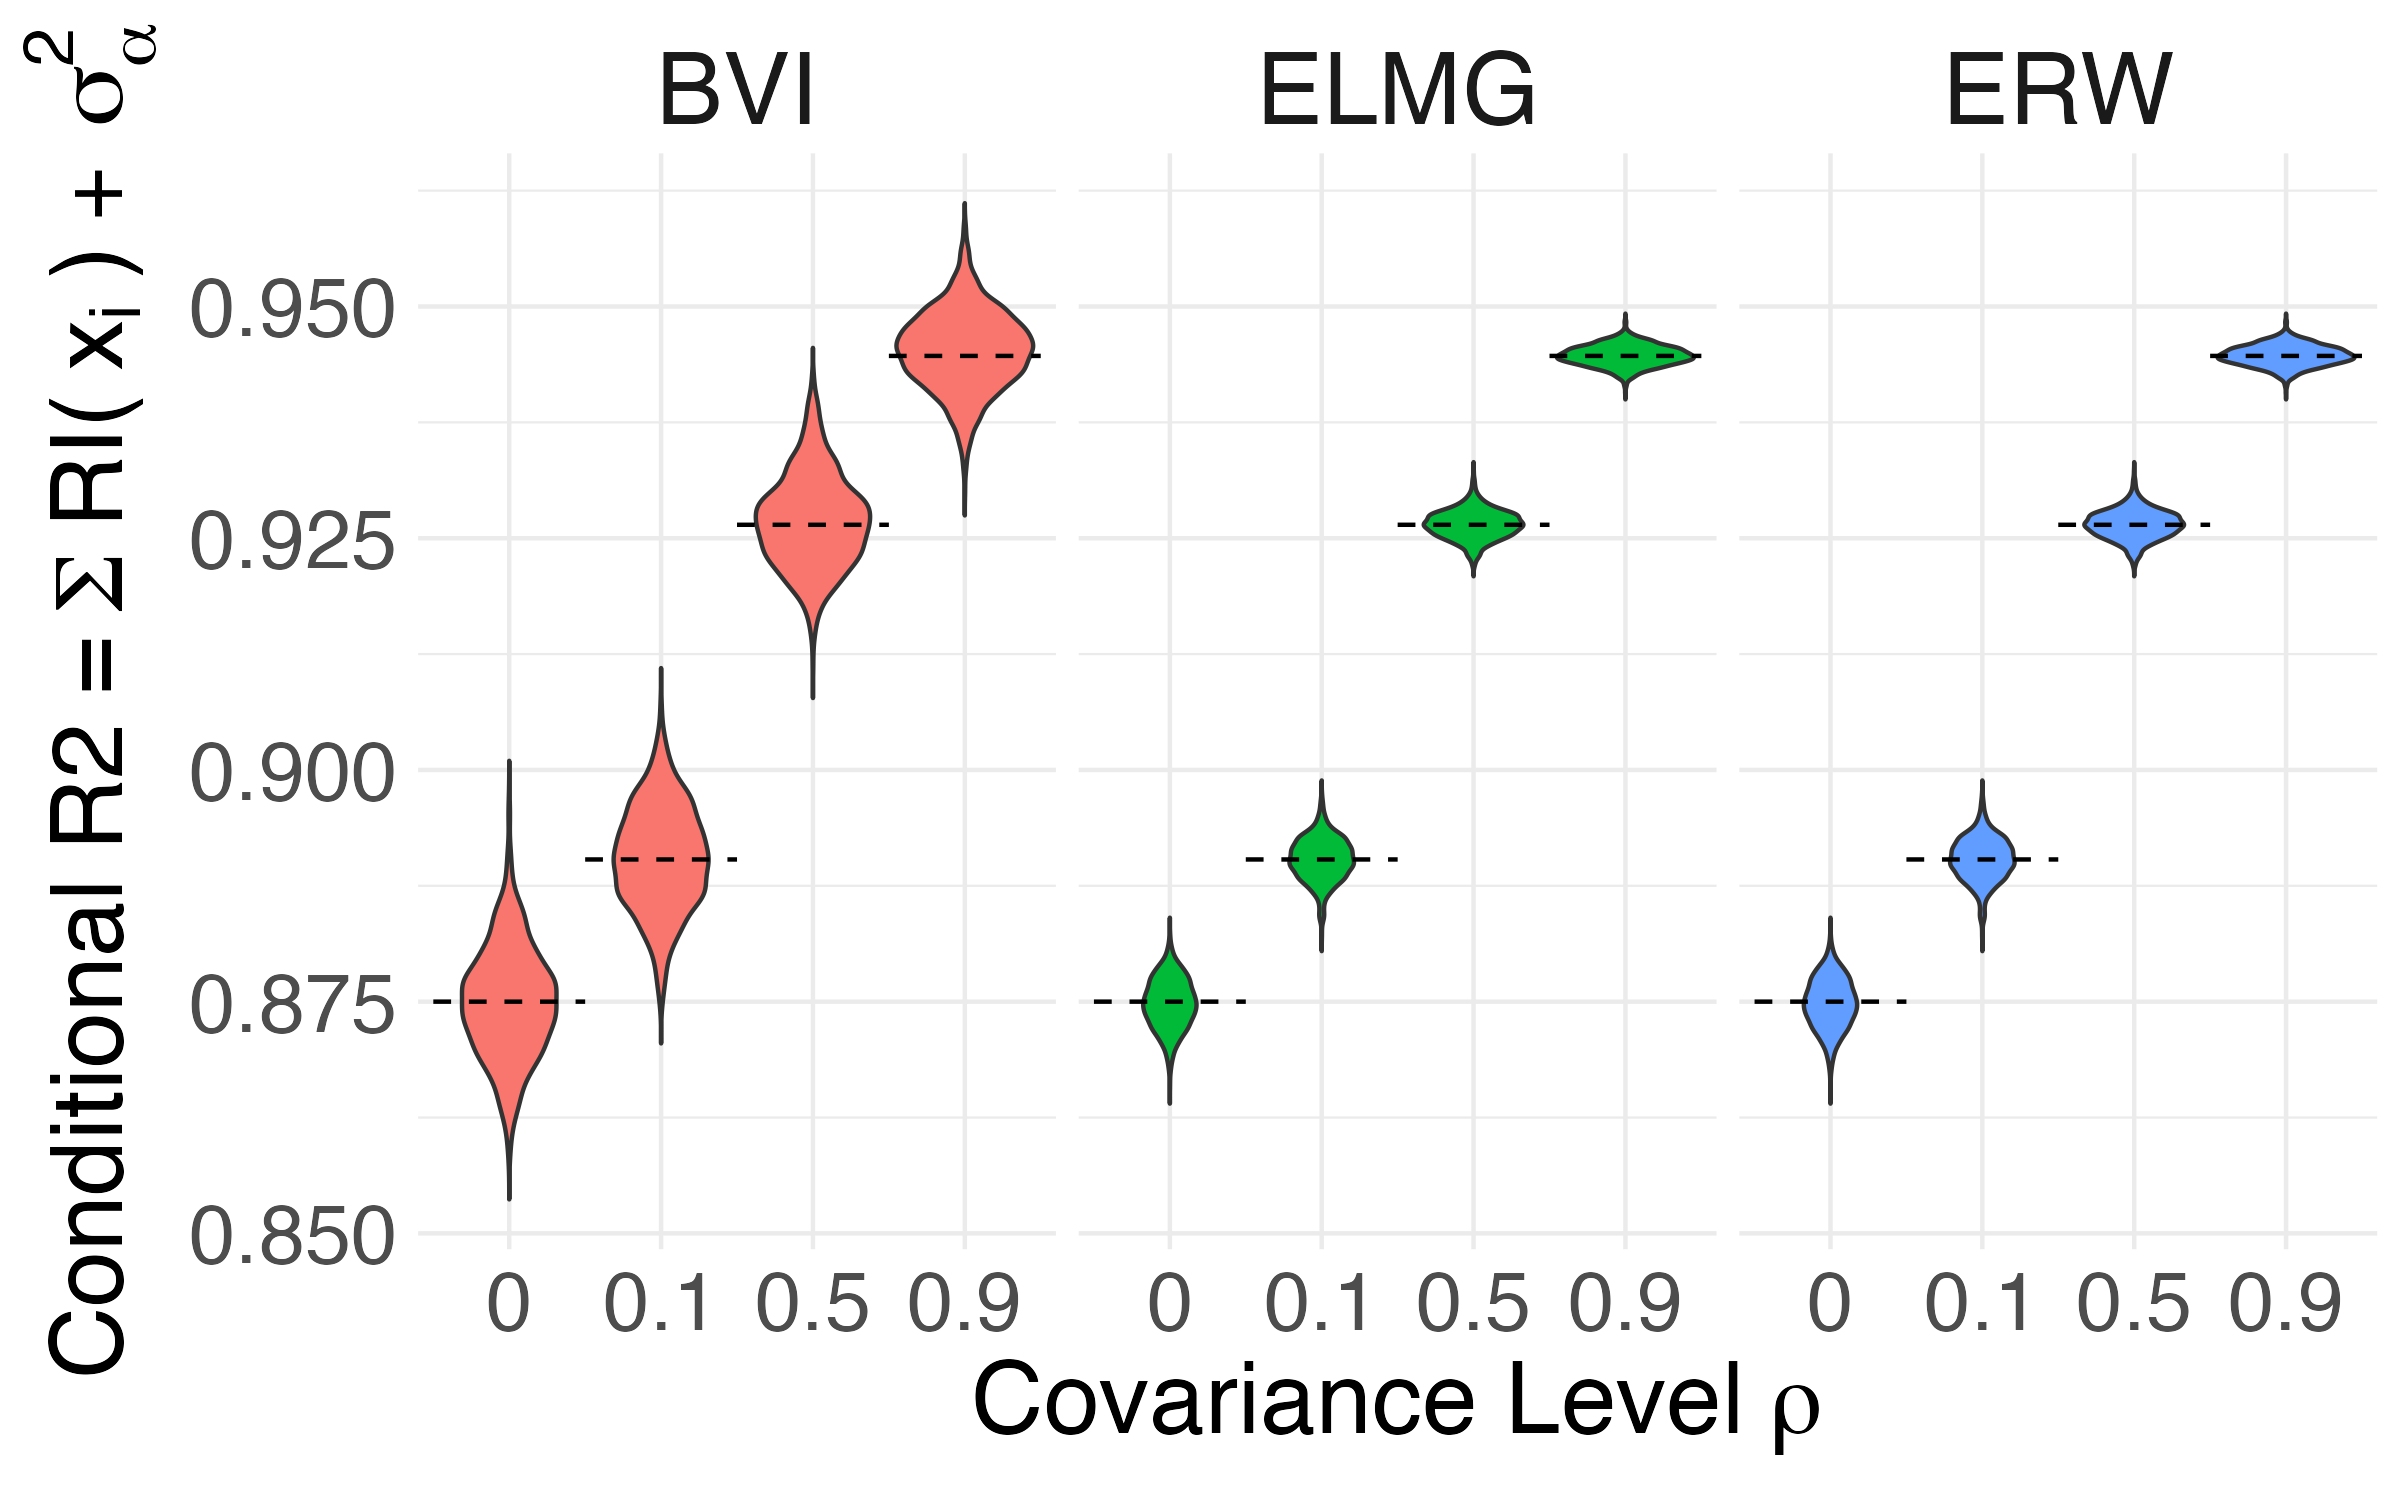
\includegraphics[width=0.6\linewidth]{Figures/ViolinPlots/Conditional_Variance.png}
    \label{fig:variance_conditional}
  }
  \caption{Violin plots for the total marginal and conditional variance explained for different correlation levels calculated from the ensemble of simulated datasets by the BVI, ELMG, the ERW and the Relaimpo method(only marginal variance explained can be computed). For the BVI method the posterior means of the sampled posterior distributions of $\boldsymbol{\beta}$ and the marginal distribution of $\hat{\sigma}^2_{\alpha}$ in each simulation are used to compare to the point estimates of the other two methods. The horizontal lines display the theoretical explained variance for each correlation level $\rho$ as in \Cref{table:1}.}
  \label{fig:total_variance}
\end{figure}

\newpage
\section{The BVI method}
The results from the BVI method for each dataset consists of the posterior marginal distributions of the variances of $\boldsymbol{\alpha}$ and $\boldsymbol{\varepsilon}$, as well as the approximated distribution of $\text{RI}(\mathbf{X})$ from samples $\boldsymbol{\beta}_{s, \mathbf{Z}}$ drawn from the joint posterior distribution $\pi(\boldsymbol{\beta}_{\mathbf{Z}}, \hat{\sigma}^2_{\alpha}, \hat{\sigma}^2_{\varepsilon} \lvert \mathbf{y})$.
The derivation of these results are described in detail in \Cref{sec:BVI_handling} and provides a more informative basis to make inference on compared to point estimation.
As this is the key advantage of the Bayesian framework, we also take a look on what results our method provides for a single model fit for different correlation levels. 
We calculate these posterior distributions for the same four different correlation levels as we use in the simulation study.
Further, we use the samples $\boldsymbol{\beta}_{s, \mathbf{Z}}$ from the joint distribution and the marginal posterior variances of $\boldsymbol{\alpha}$ and $\boldsymbol{\varepsilon}$ to calculate the distribution of $R^2$ in accordance with \eqref{eq:R2_bayes_LMM_cond} and \eqref{eq:R2_bayes_LMM_marg}. 

\subsection{Posterior relative importance distributions}
\label{sec:posterior_distributions}
Approximate posterior marginal distributions for the variances of the random effects, and sampled approximate posterior distributions for the fixed effects are available for the BVI method for each dataset.
These are featured in \Cref{fig:posterior_distributions} for one realization of the four different datasets of different correlations.
All posteriors for one correlation level are shown in the same subplot, with one subplot for each correlation level. 
For the correlation level $\rho=0$ the theoretically correct relative importances are shown as vertical lines.
Note here that it is expected and desired that the distributions from a single dataset are stochastic and therefore deviate somewhat from the theoretical values.
When data are uncorrelated (\Cref{fig:posteriors_none}) the posterior distributions are coincidentally centered close to the theoretical value.
The posterior distribution of $\hat{\sigma}^2_{\alpha}$ is slightly skewed to the left and demonstrates a distinctively larger degree of dispersion than the other effects.
For $\rho=0.1$ (\Cref{fig:posteriors_low}), a small shift of all posterior distributions is noticeable, in accordance with the results from \Cref{fig:relimp_X1} and \Cref{fig:relimp_alpha}. 
This repositioning is more clear for $\rho=0.5$ and $\rho=0.9$ (\Cref{fig:posteriors_medium} and \Cref{fig:posteriors_high}), and it is clear to see that the posterior distribution of the variance of $\hat{\sigma}^2_{\alpha}$ follows the trend of $\hat{\sigma}^2_{\varepsilon}$ closely.
When correlation is increased, it seems that the width of all posterior distributions narrow and become tighter.
The trend of increasing relative importance assigned to $X_1$ and $X_2$ while decreasing importance assigned to $X_3$ is highlighted by the posterior distributions of the respective effects as they align closer for each increase in correlation.
These are the types of results that we would expect to see, as they deviate from the theoretical values with a plausible amount when considering that they are stochastic.
\begin{figure}[!ht]
  \centering
  % First row
  \subfloat[$\rho=0$]{
    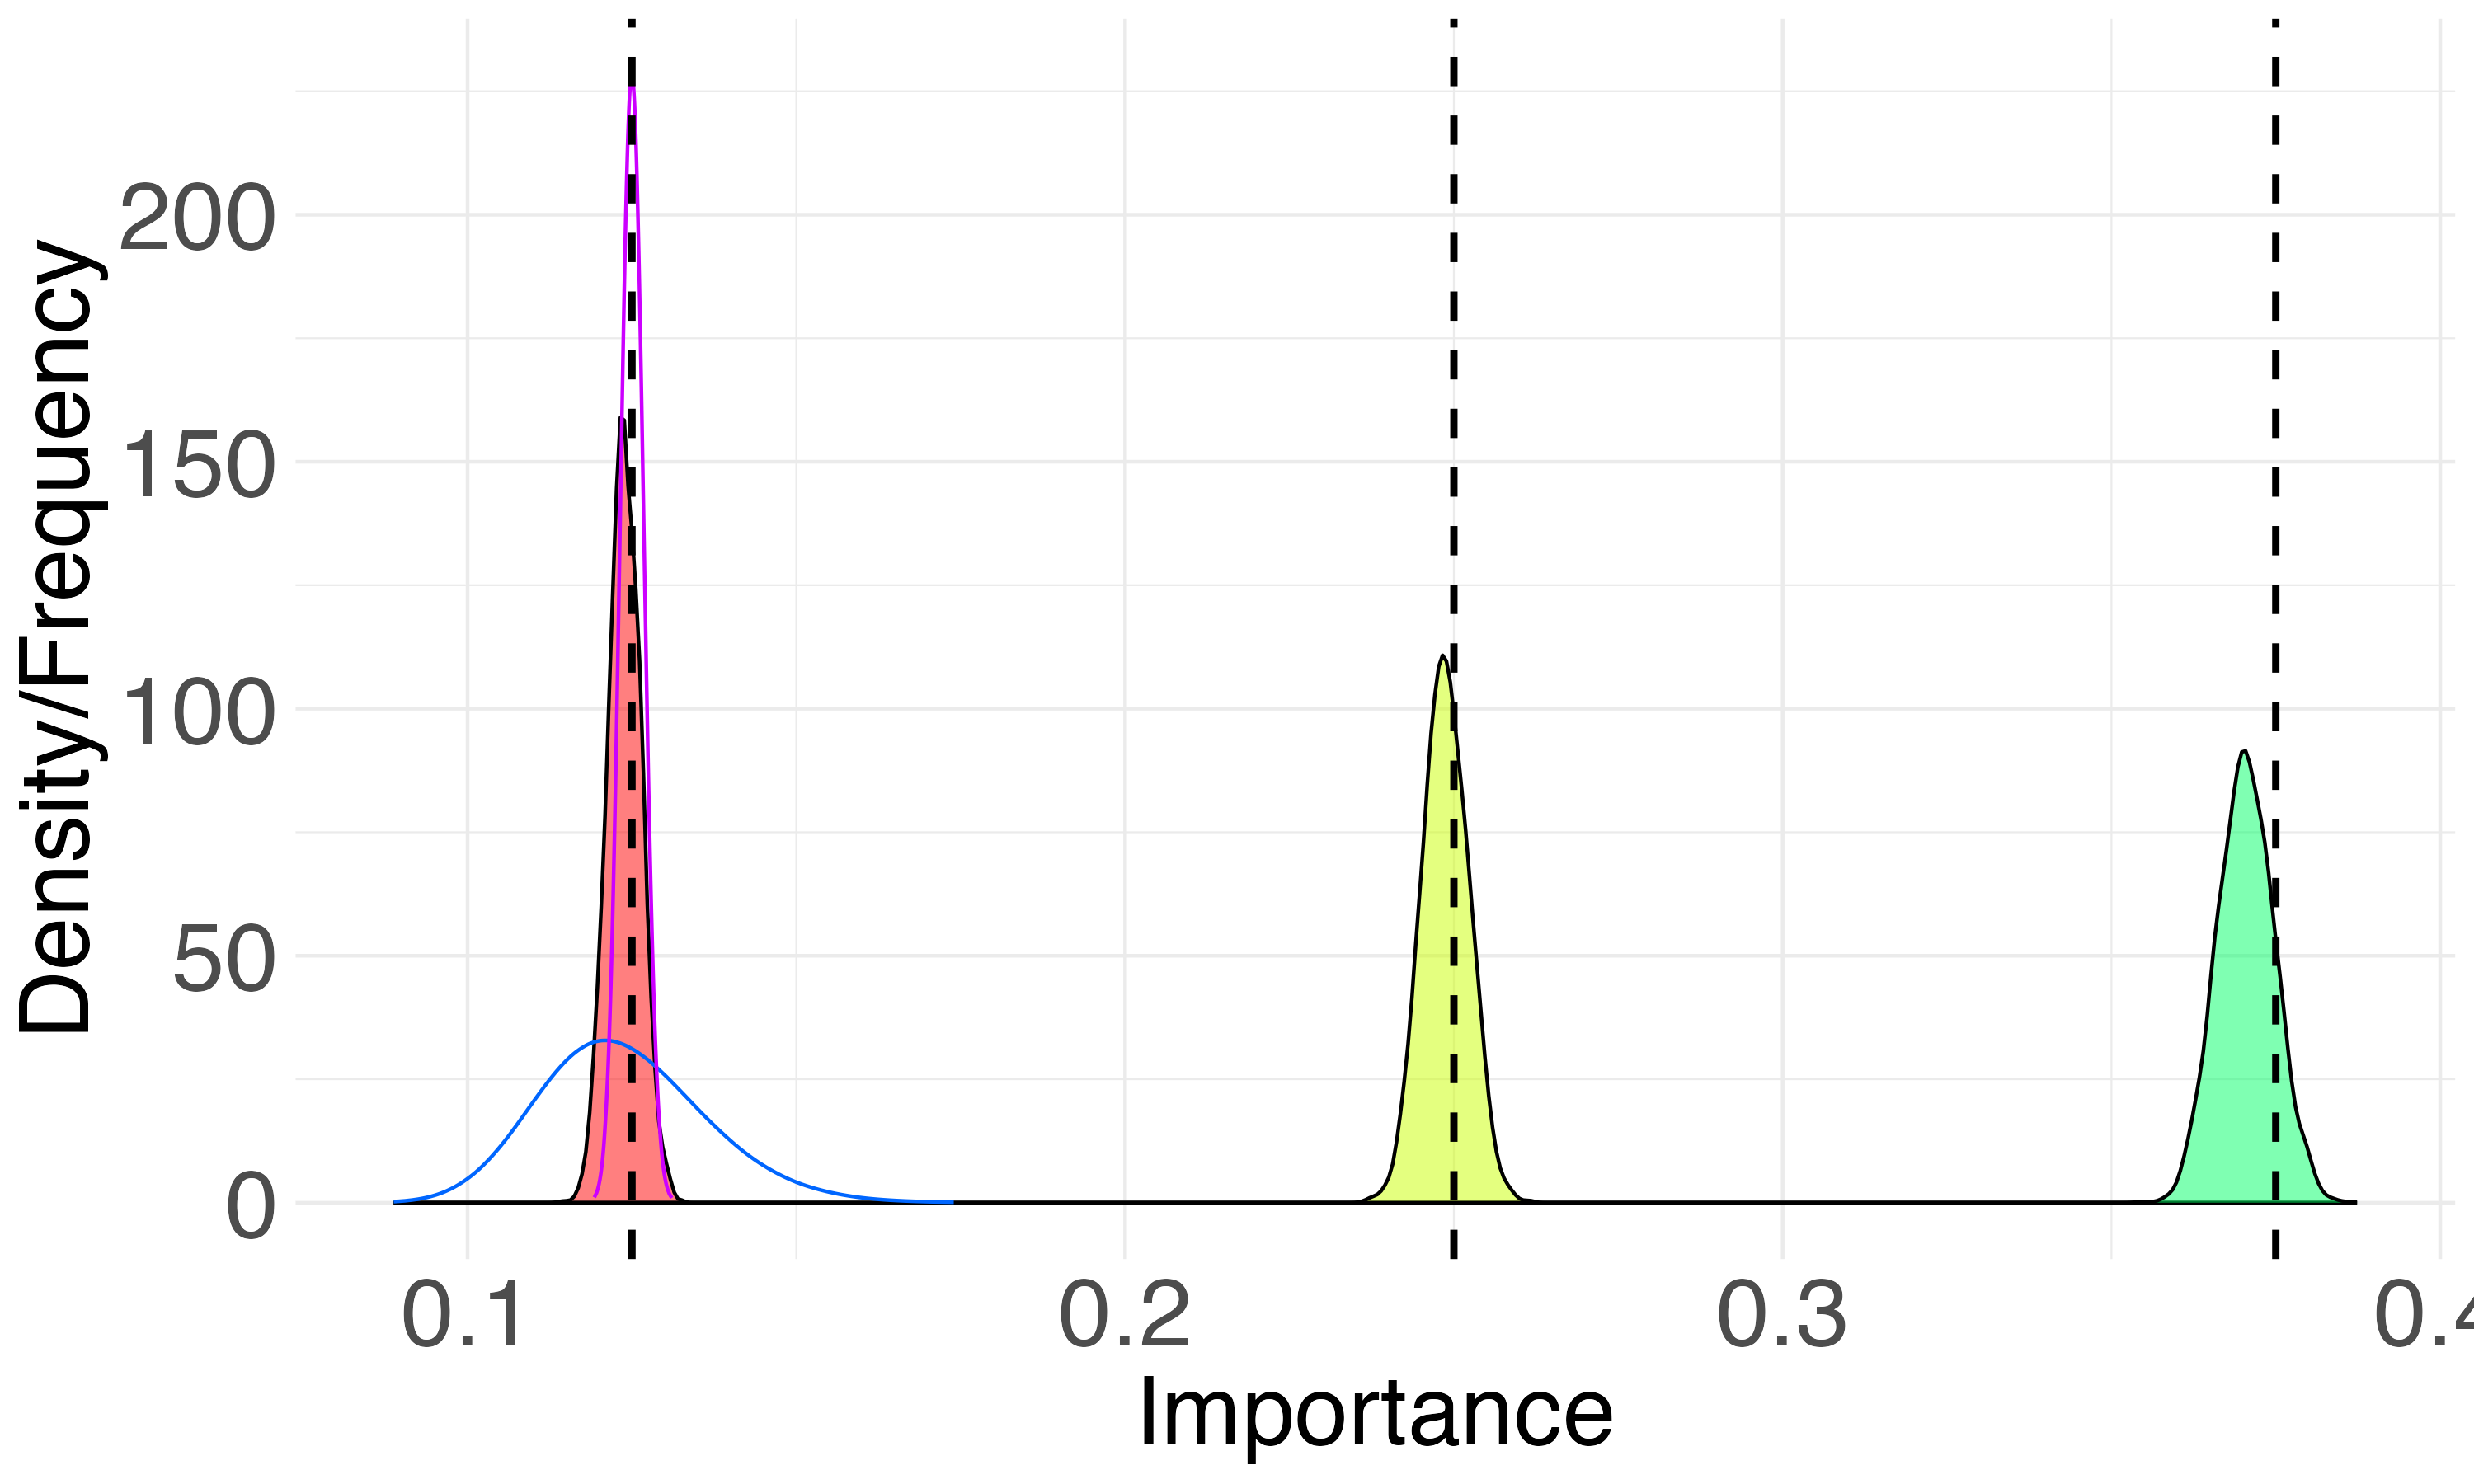
\includegraphics[width=0.5\linewidth]{Figures/Posterior Marginal/Posterior importance, cov=none.png}
    \label{fig:posteriors_none}
  }
  \subfloat[$\rho=0.1$]{
    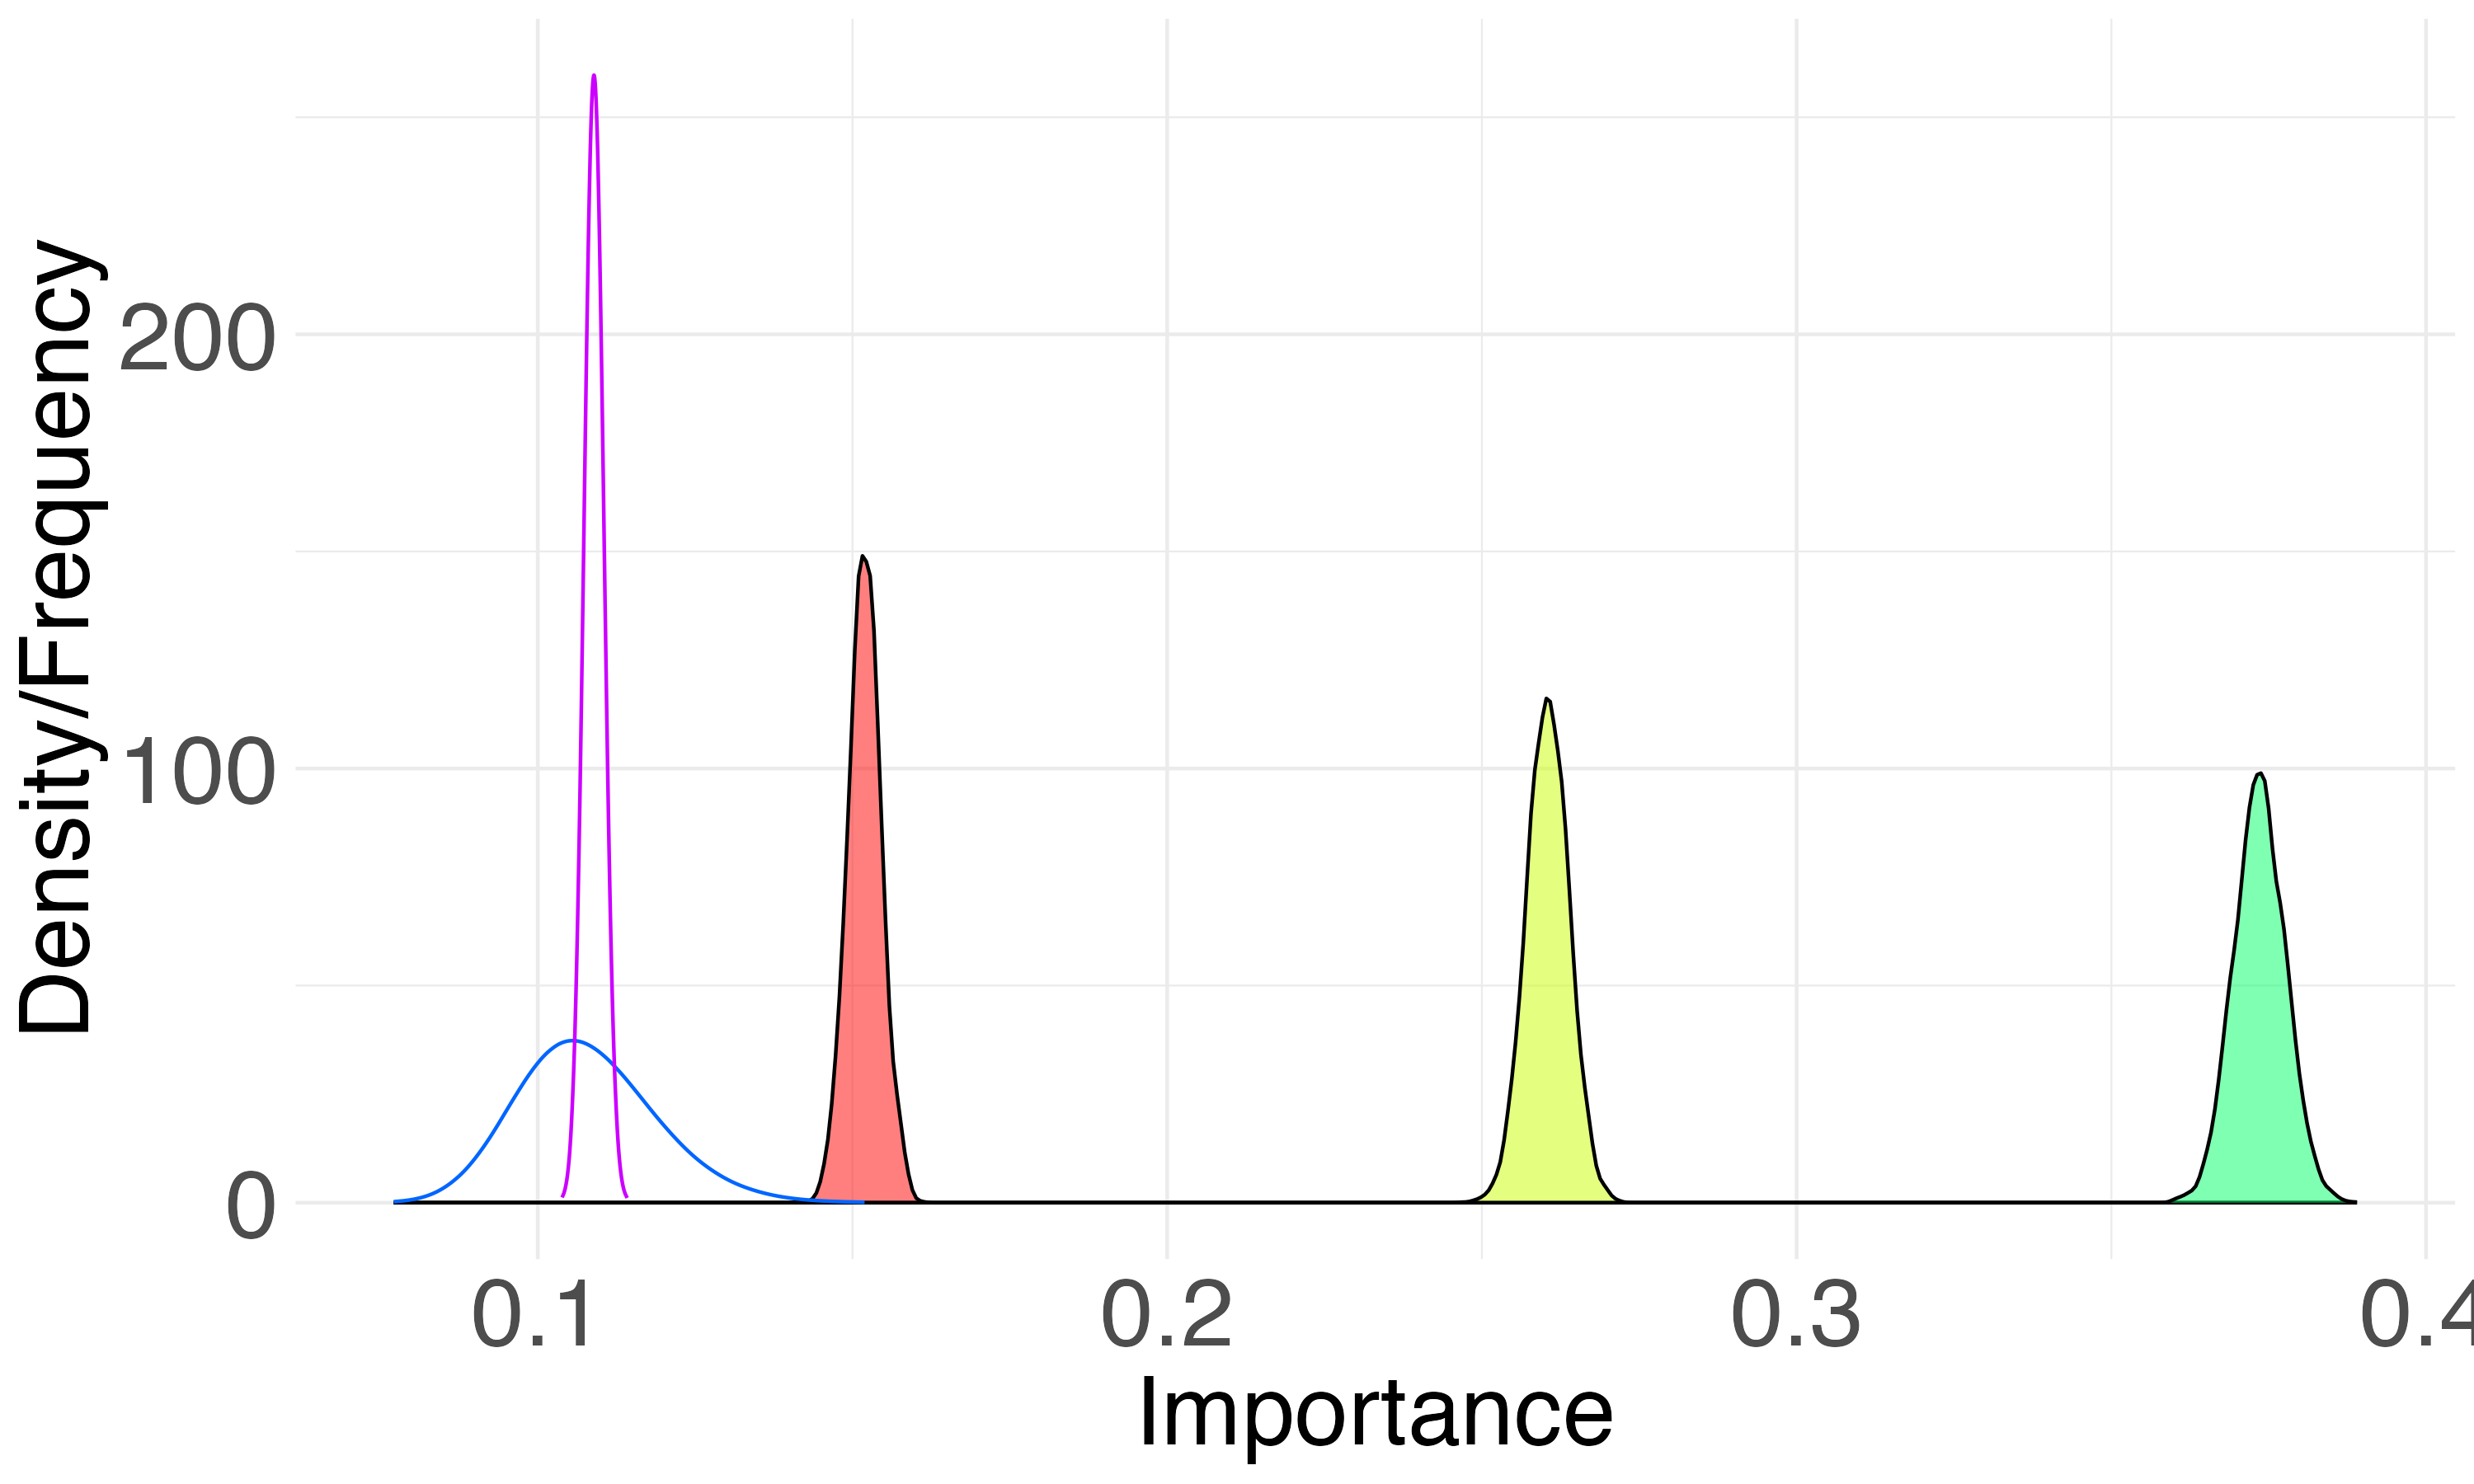
\includegraphics[width=0.5\linewidth]{Figures/Posterior Marginal/Posterior importance, cov=low.png}
    \label{fig:posteriors_low}
  }
  \vspace{5mm}
  % Second row
  \subfloat[$\rho=0.5$]{
    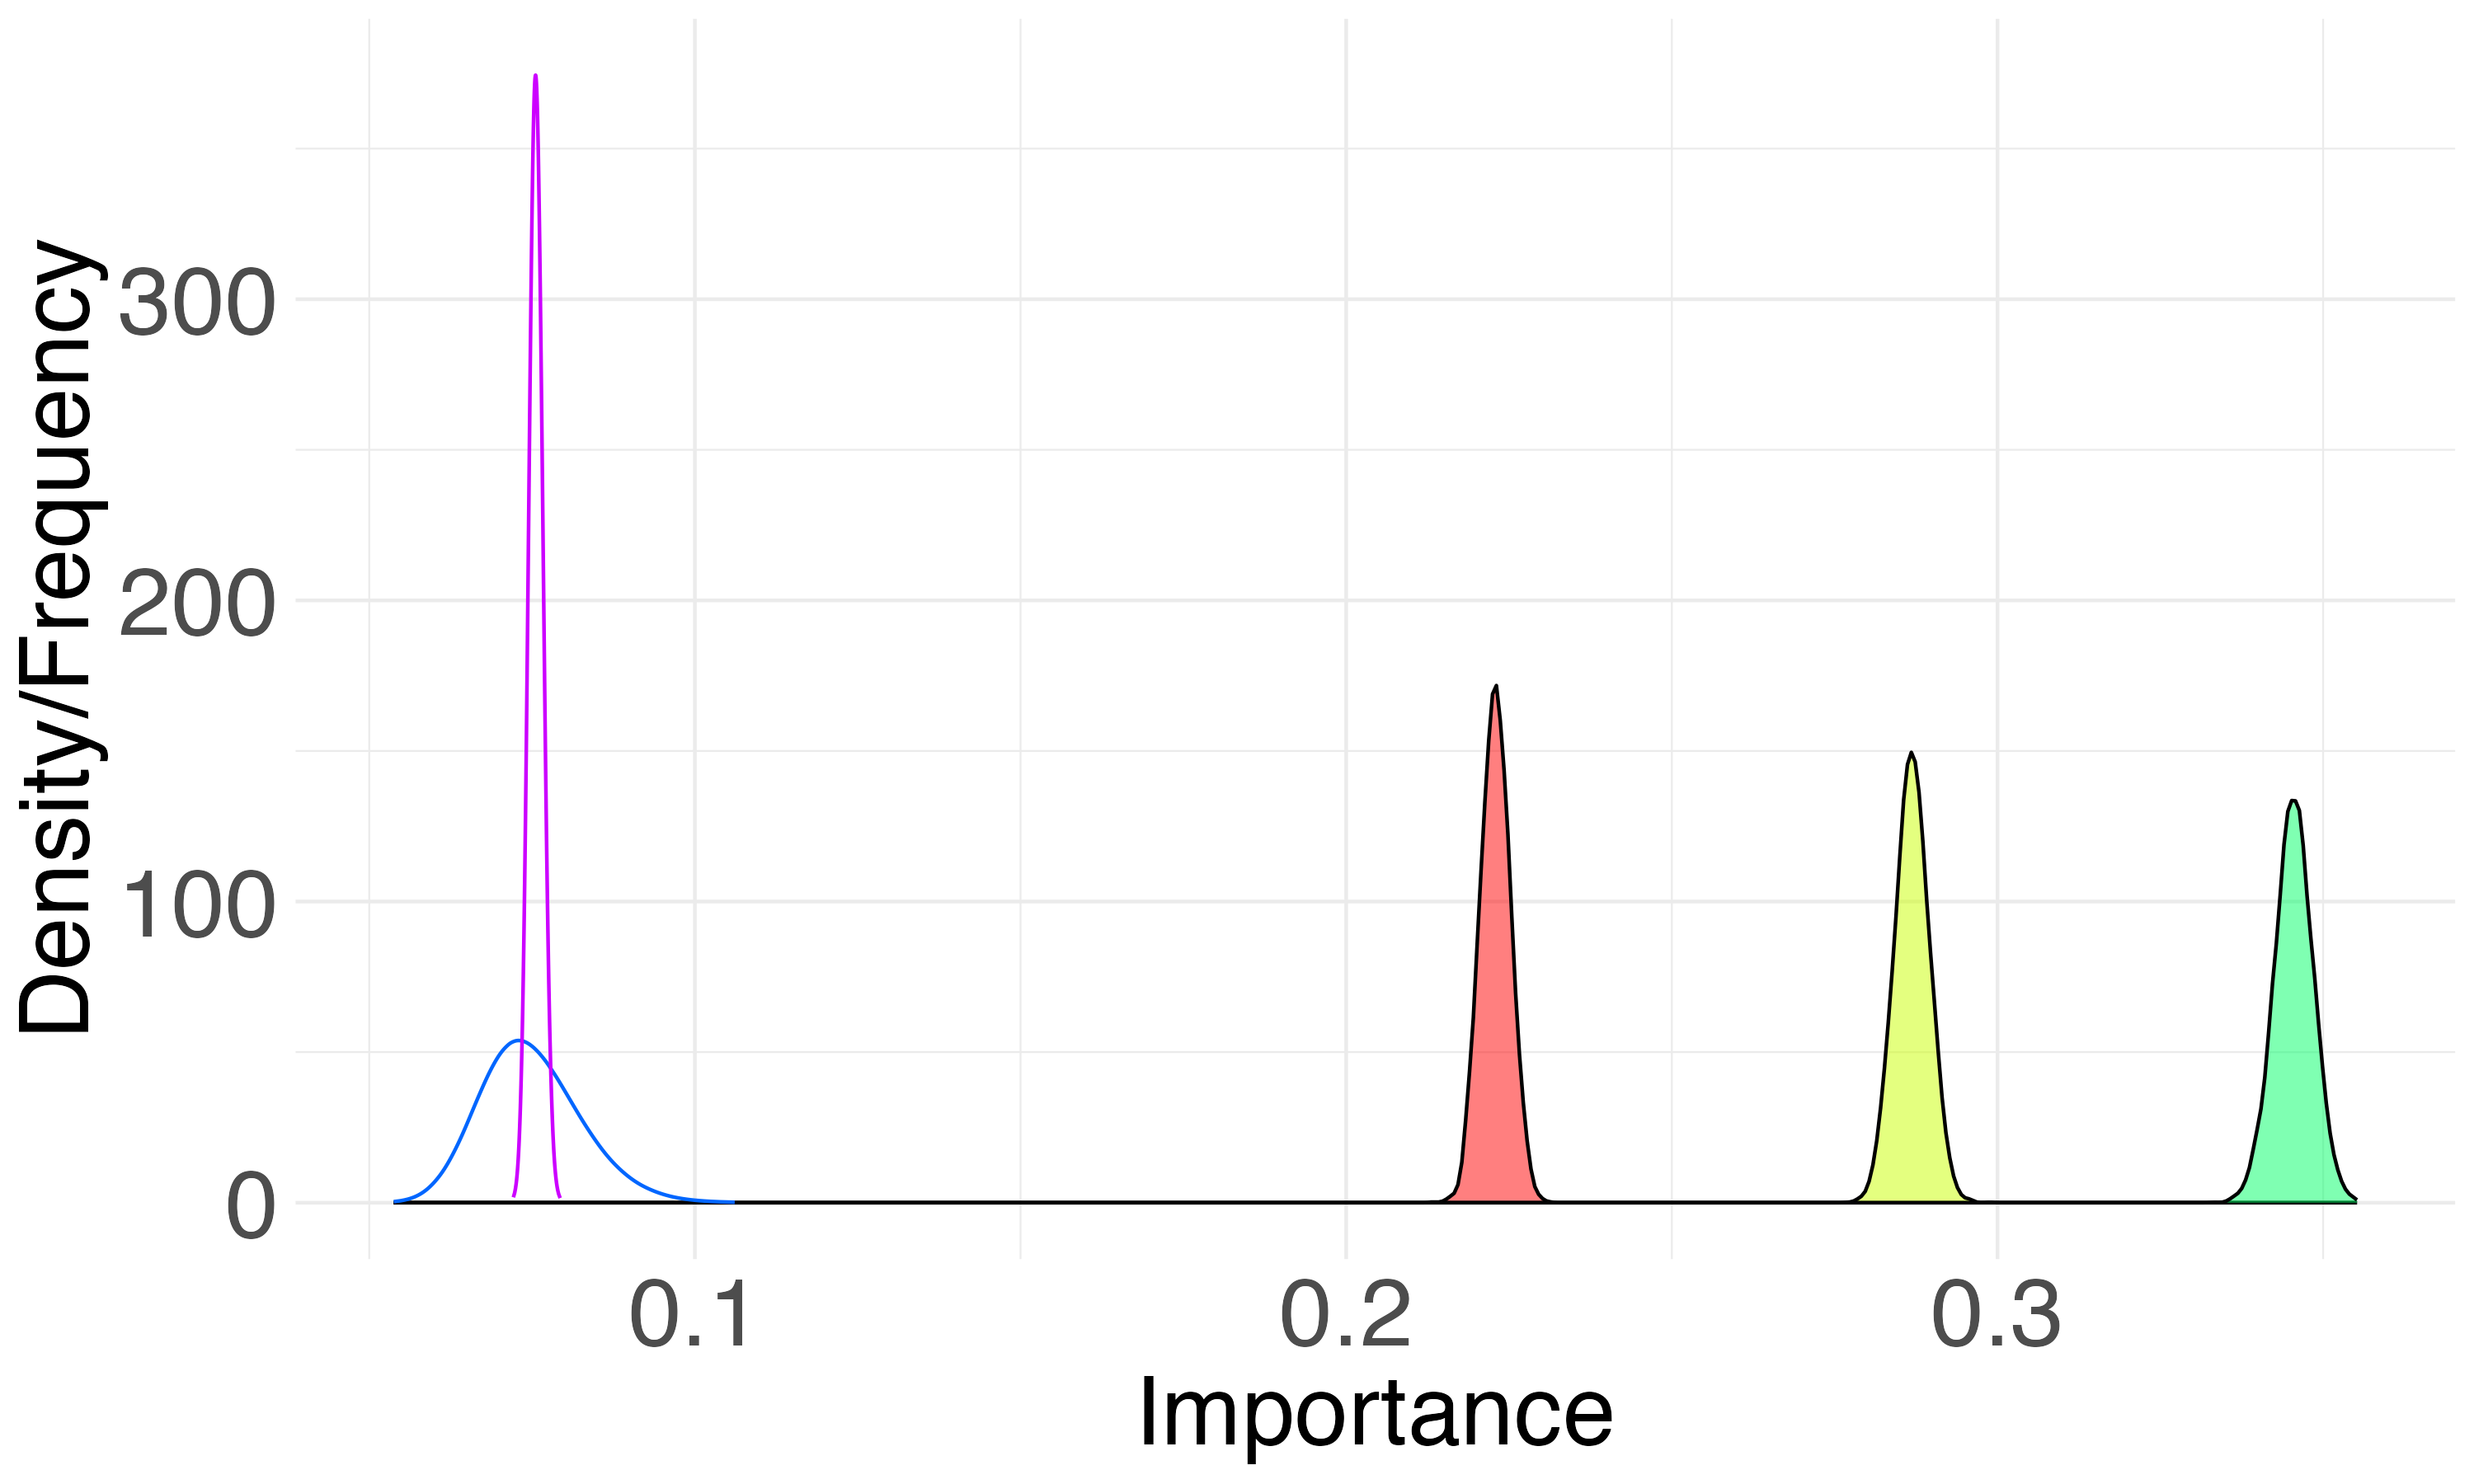
\includegraphics[width=0.5\linewidth]{Figures/Posterior Marginal/Posterior importance, cov=medium.png}
    \label{fig:posteriors_medium}
  }
  \subfloat[$\rho=0.9$]{
    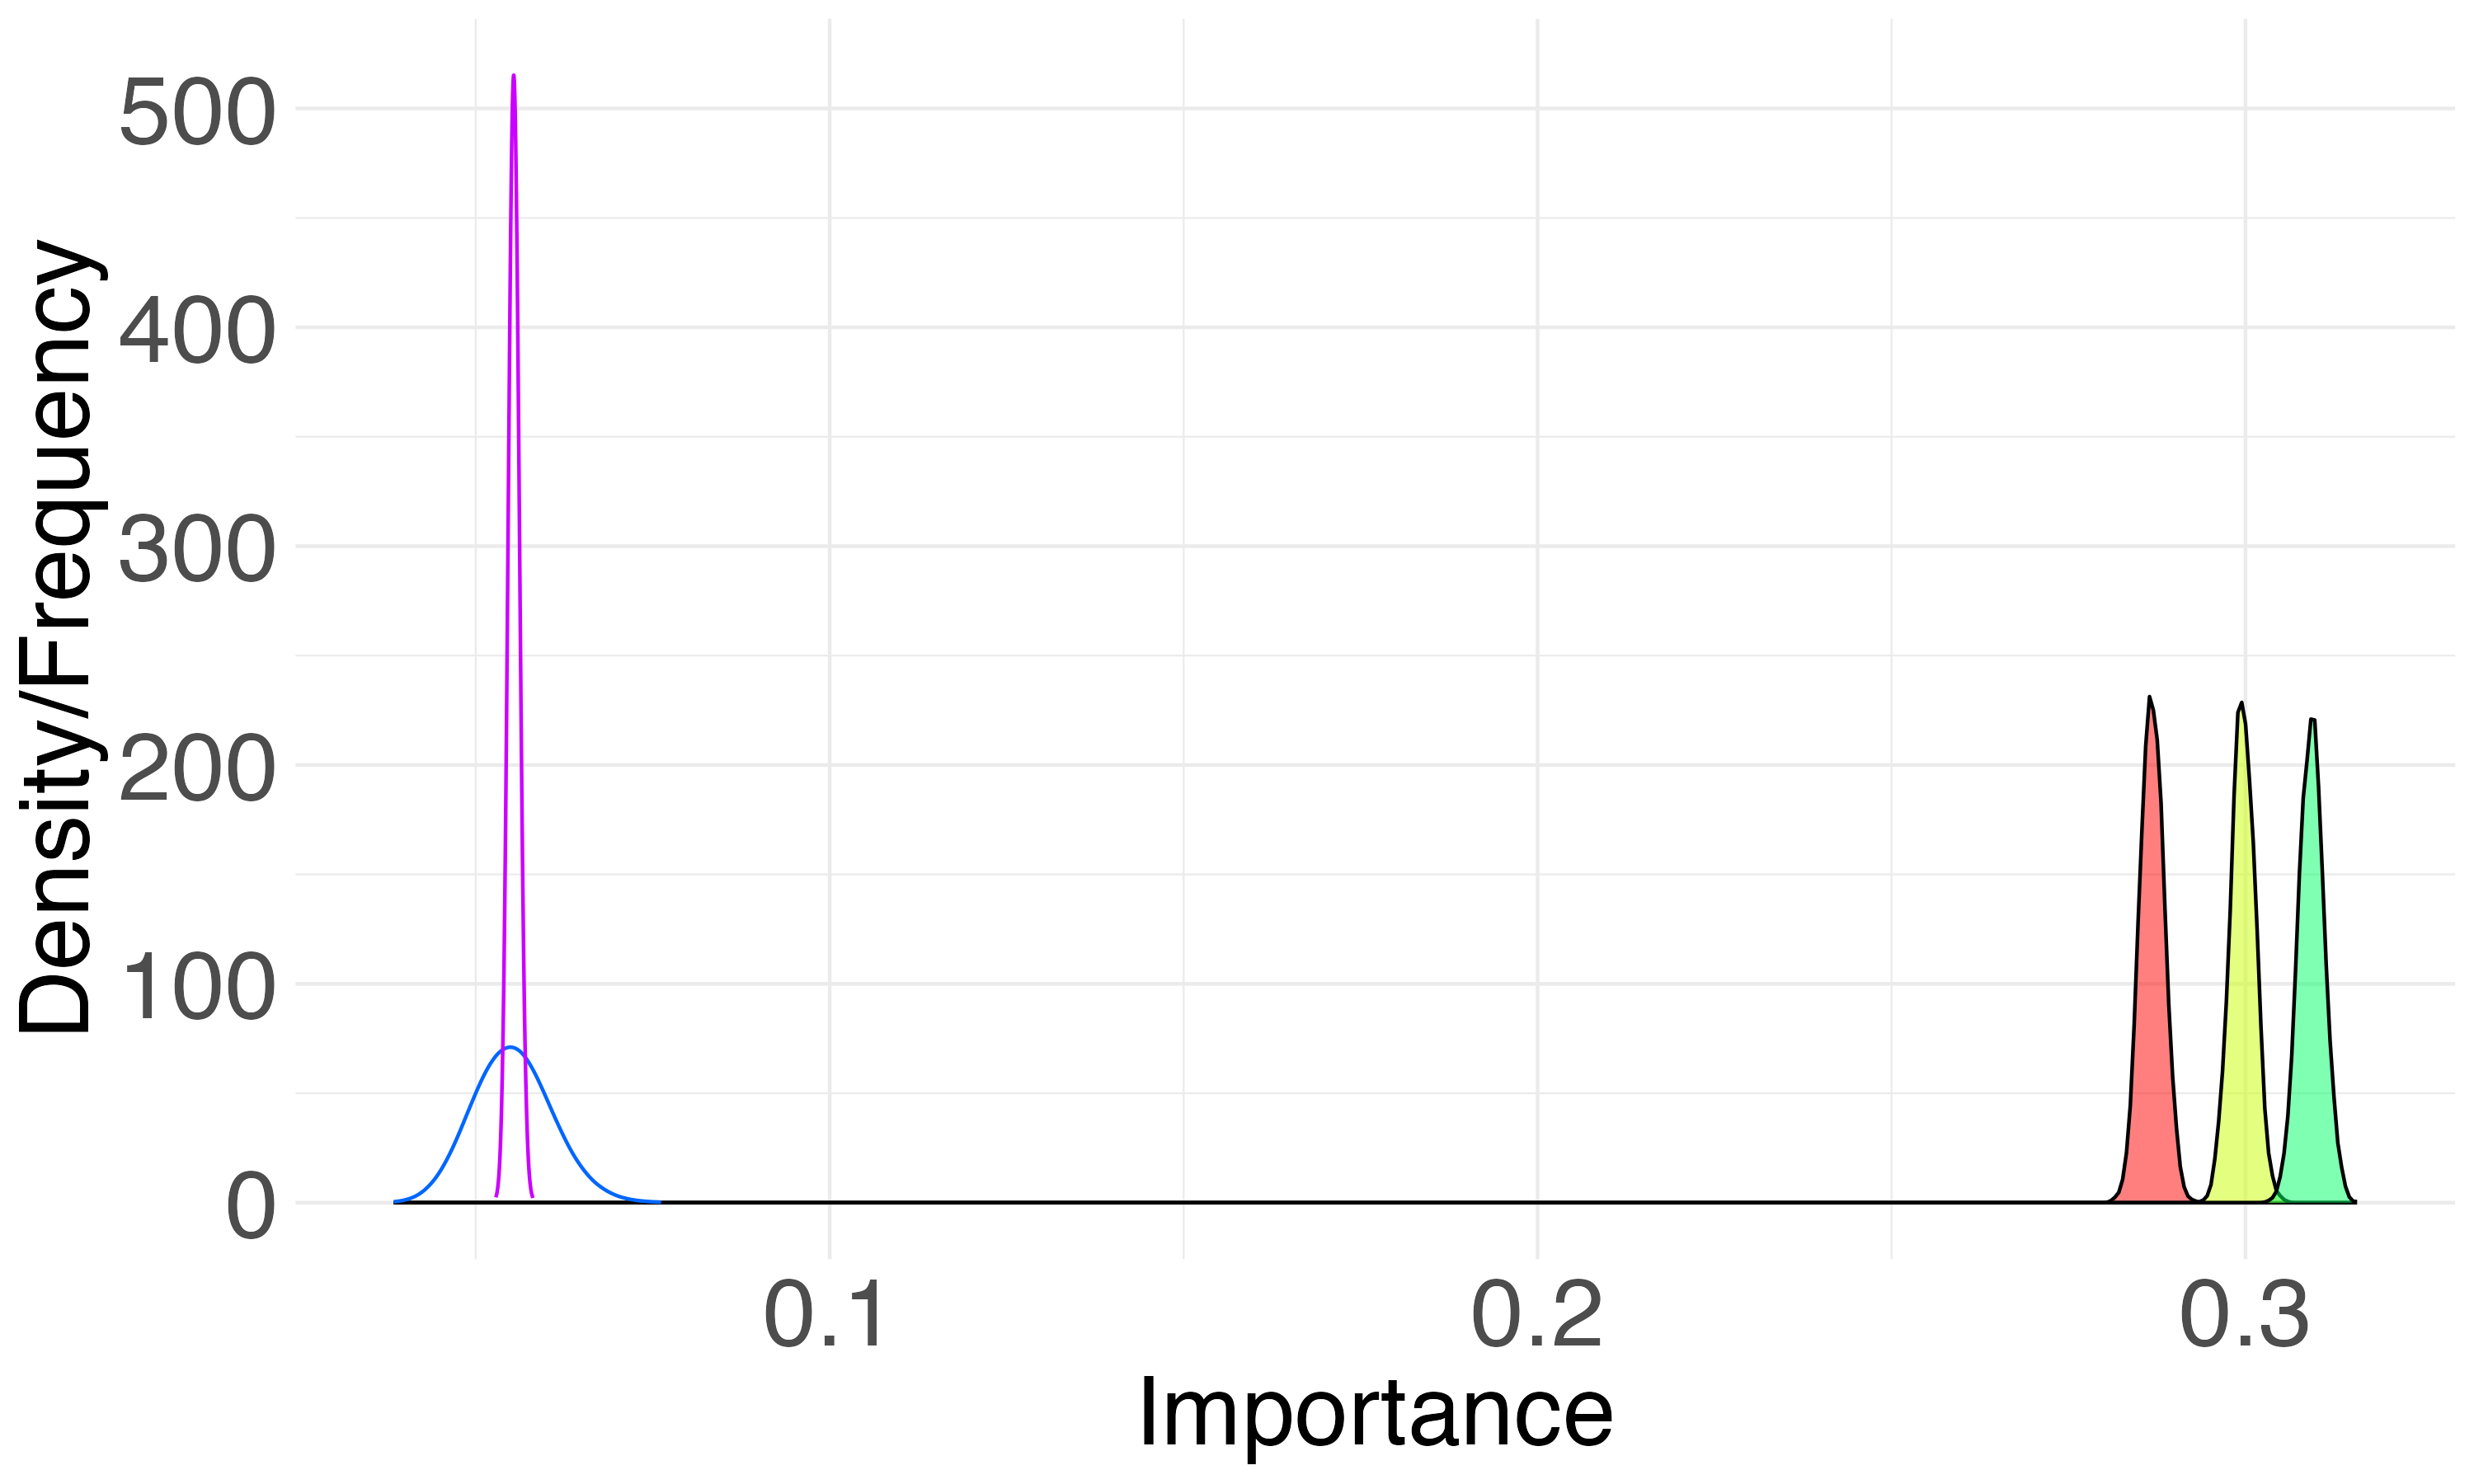
\includegraphics[width=0.5\linewidth]{Figures/Posterior Marginal/Posterior importance, cov=high.png}
    \label{fig:posteriors_high}
  }

  \caption{Posterior distributions for fixed effects and posterior marginal distributions for random effects from the BVI method on four randomly simulated datasets with different correlation values between the fixed effects. The blue and purple densities are the marginal posteriors for $\hat{\sigma}^2_{\alpha}$ and $\hat{\sigma}^2_{\varepsilon}$ respectively, whereas the red, yellow and green densities are the sampled posteriors for $X_1, X_2$ and $X_3$ respectively. The vertical lines in (a) represent the theoretically correct relative importances.}
  \label{fig:posterior_distributions}
\end{figure}
\newpage
\subsection{Posterior $R^2$ distributions}
From the above discussed posterior distributions, the posterior distributions of marginal (\Cref{fig:marginal_R2}) and conditional (\Cref{fig:conditional_R2}) variance explained, \textit{i.e.} $R^2$, can also be obtained.
As was the case for the posterior distributions of fixed and random effects, the $R^2$ distributions are also desired to possess a degree of stochasticity causing them to deviate moderately from the theoretical value.
We notice that in the uncorrelated case the $R^2$ is evenly distributed around the theoretically expected variance explained. 
For $\rho=0.1$ and $\rho=0.9$ the distribution of $R^2$ seem to be a skewed to the right when comparing it to the theoretically expected value and the distribution for $\rho=0.5$ skewed to the left.
The width of the distributions seem to narrow as correlation levels increase, as a result of the decreasing width in the individual posterior distributions of random and fixed effects.
\newline
\newline
Moving on to the conditional $R^2$ (\Cref{fig:conditional_R2}), which are displayed on the same scale as the marginal $R^2$, it is obvious that these distributions are tighter than the marginal $R^2$ distributions.
The scale is arguably too large to be used to display the conditional $R^2$ when one sees how narrow they are, but we chose to do so because of the comparison to the marginal $R^2$.
To the contrary, for $\rho=0.1$ and $\rho=0.9$ the distributions are skewed to the right. 
The marginal and conditional $R^2$ for the same model will be closely related so one should expect to see the same behaviour in both, as we do.
\newline
\newline
The posterior distributions of $R^2$ reflect our expectations as they exhibit the same stochasticity as seen for the posterior distributions of fixed and random effects.
\begin{figure}[H]
  \centering
  % First row
  \subfloat{
    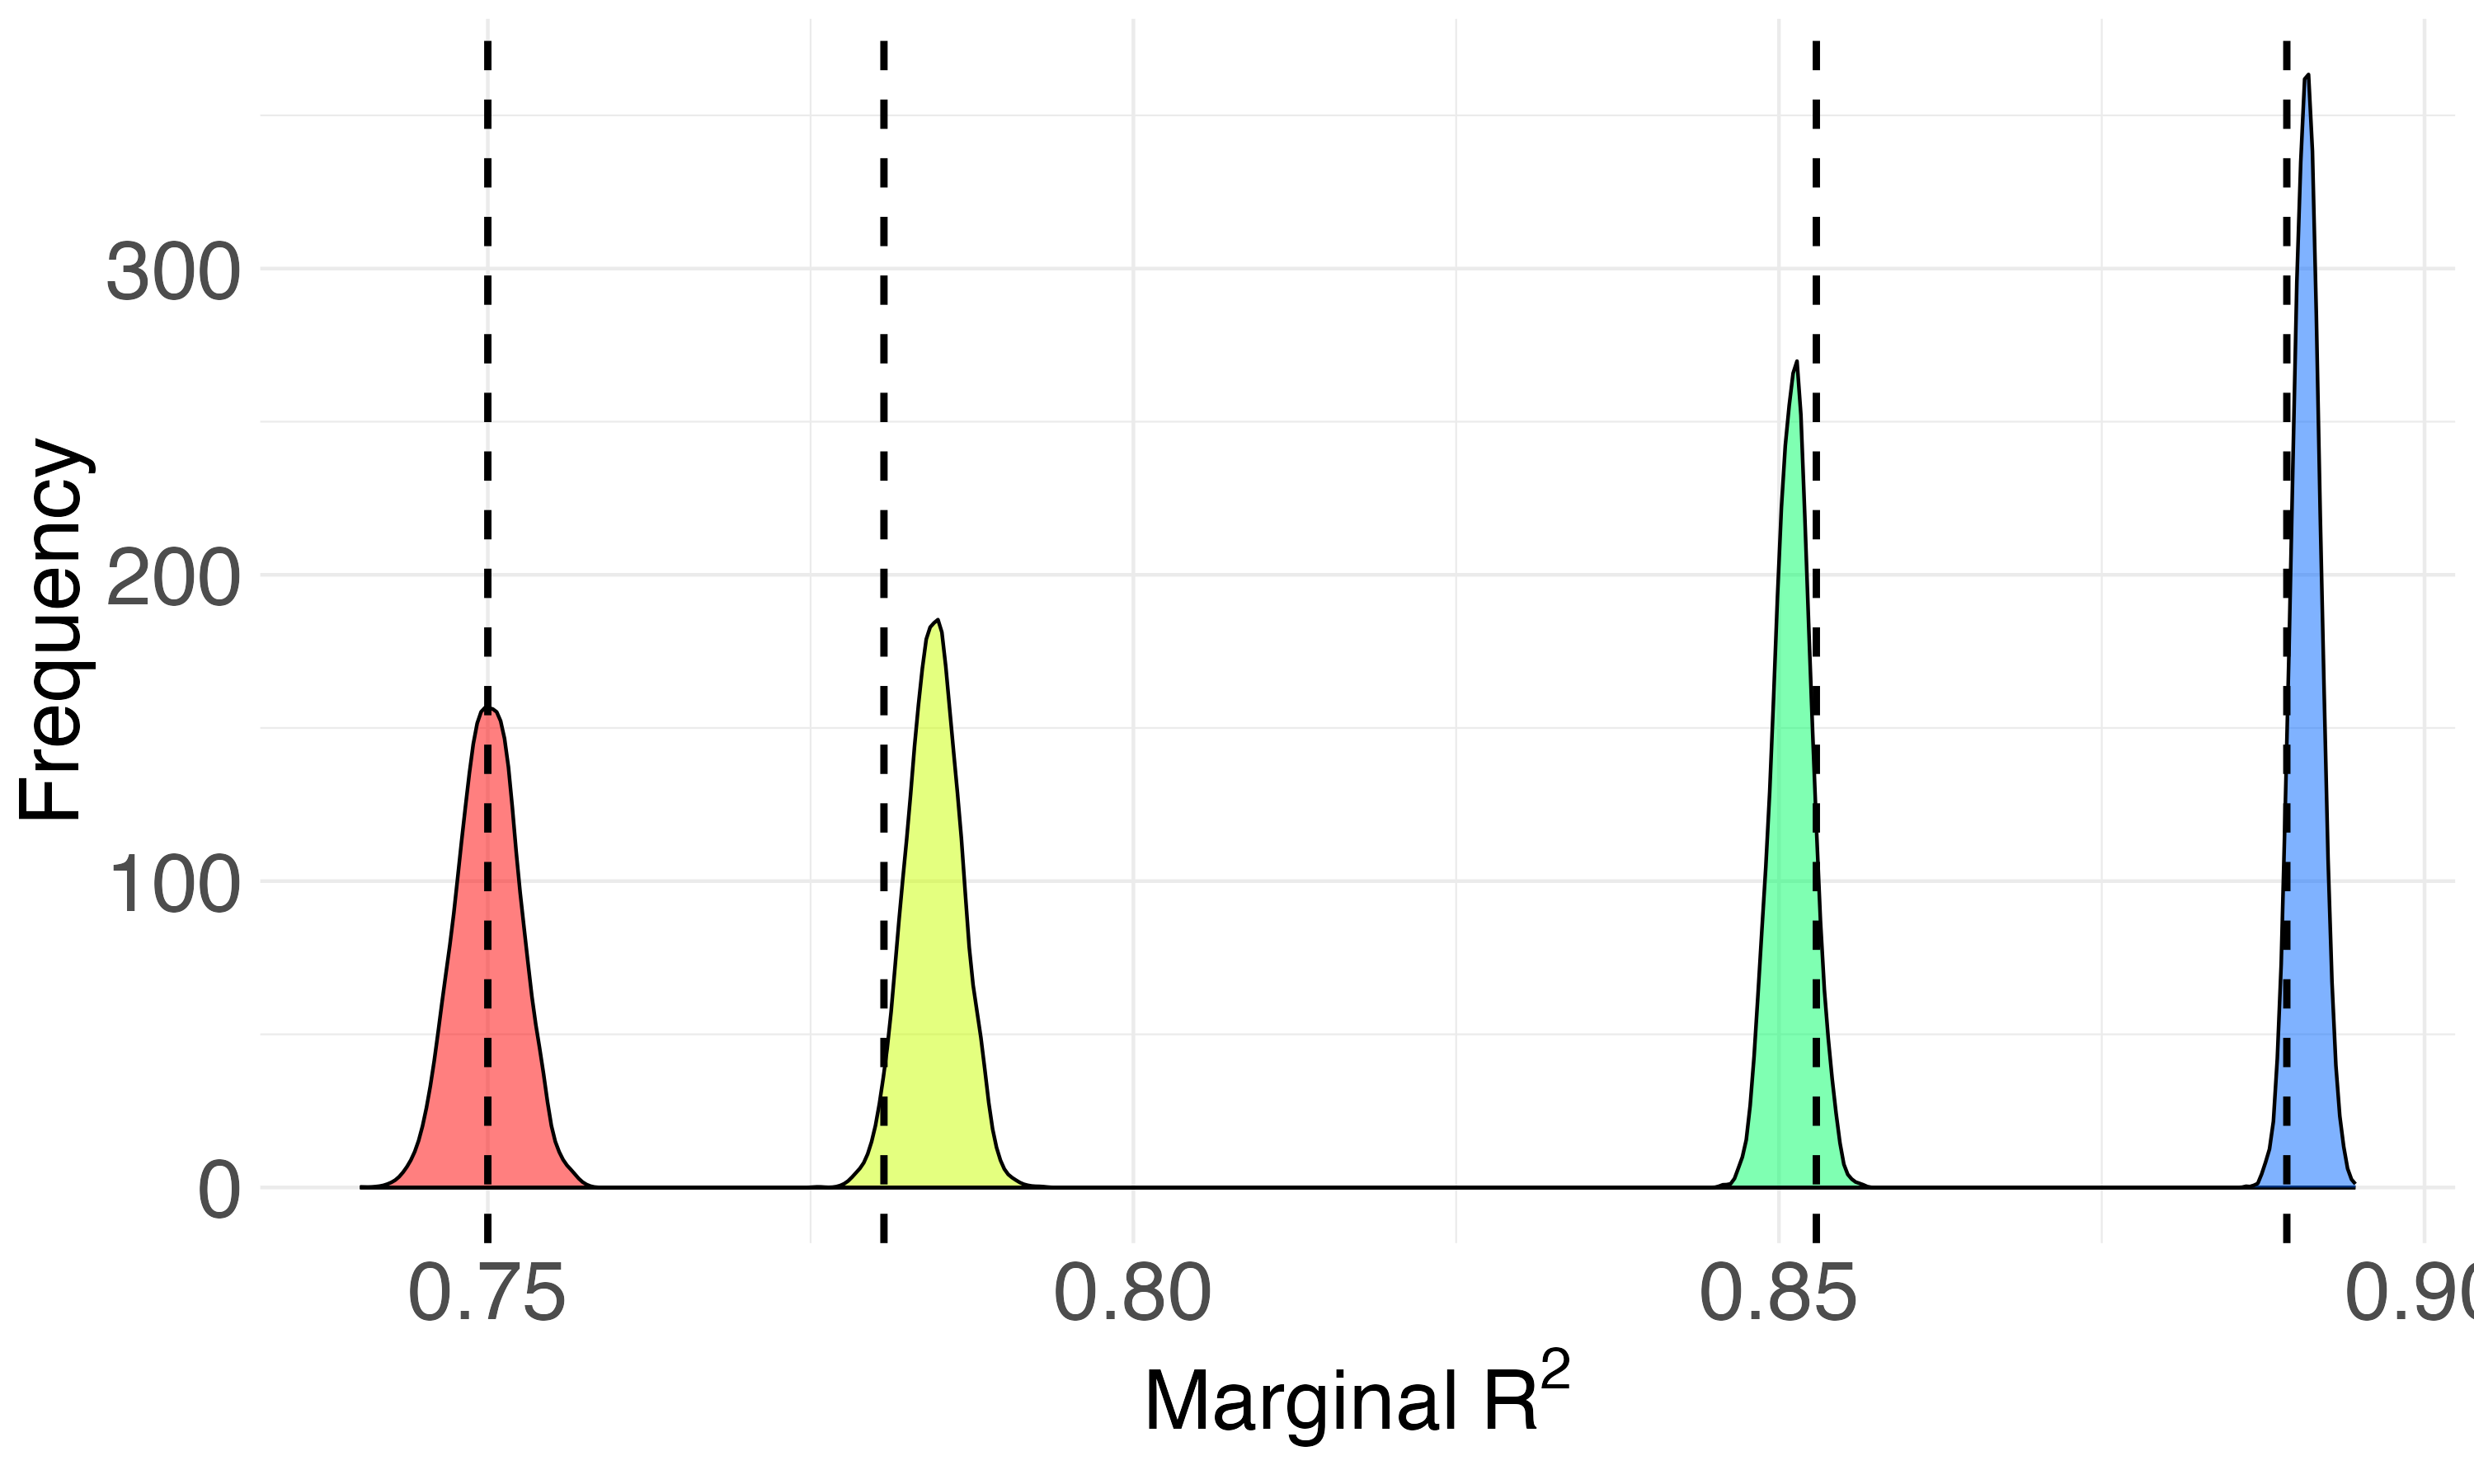
\includegraphics[width=0.7\linewidth]{Figures/R2/Marginal_R2.png}
    %\caption{Posterior marginal $R^2$ distribution calculated by the BVI method from the posterior distributions of fixed and random effects on four randomly simulated datasets with different correlation values $\rho$ between the fixed effects. The blue, green, red and purple distributions correspond to the posterior distribution of marginal $R^2$ for $\rho=0, \rho=0.1, \rho=0.5$ and $\rho=0.9$ respectively. The vertical lines represent the theoretically expected $R^2$ as presented in \Cref{table:1}.}
    \label{fig:marginal_R2}
  }
  \hfill
  \subfloat{
    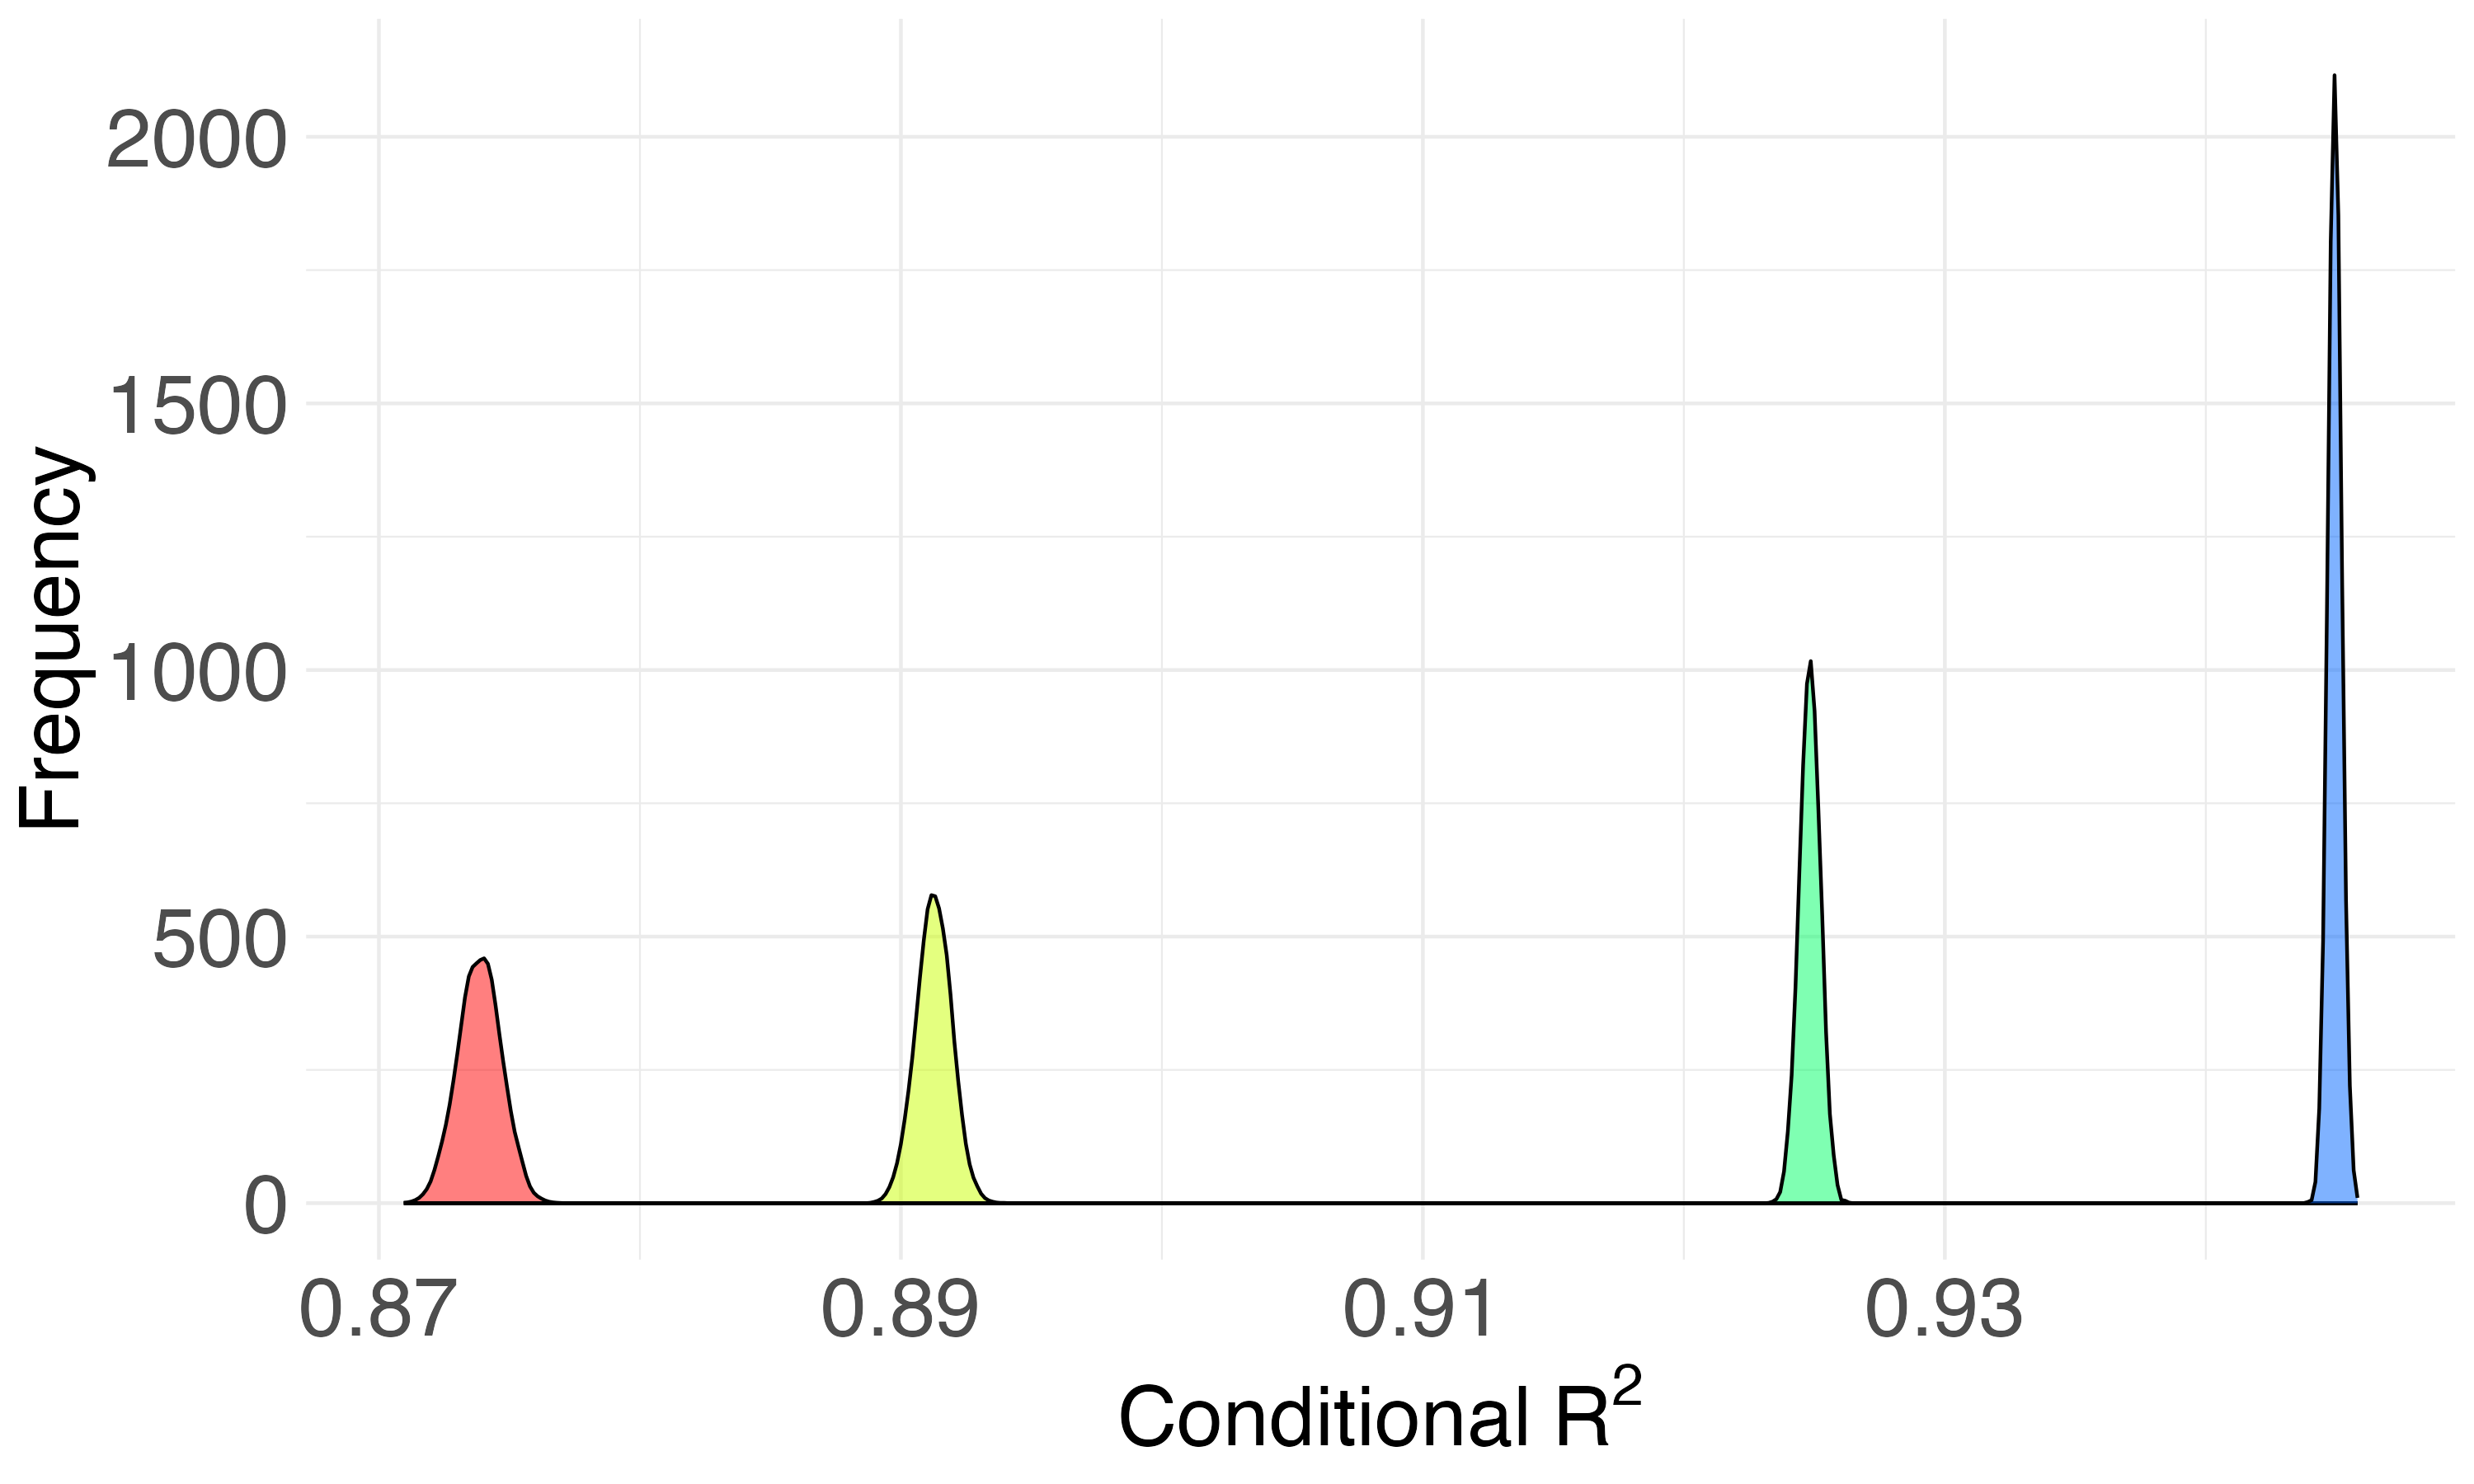
\includegraphics[width=0.7\linewidth]{Figures/R2/Conditional_R2.png}
    %\caption{Posterior conditional $R^2$ distribution calculated by the BVI method from the posterior distributions of fixed and random effects on four randomly simulated datasets with different correlation values $\rho$ between the fixed effects. The blue, green, red and purple distributions correspond to the posterior distribution of conditional $R^2$ for $\rho=0, \rho=0.1, \rho=0.5$ and $\rho=0.9$ respectively. The vertical lines represent the theoretically expected $R^2$ as presented in \Cref{table:1}.}
    \label{fig:conditional_R2}
  }
  \caption{Posterior $R^2$ distribution calculated by the BVI method from the posterior distributions of fixed and random effects on four randomly simulated datasets with different correlation values $\rho$ between the fixed effects. The red, yellow, green and blue distributions correspond to the posterior distribution of $R^2$ for $\rho=0, \rho=0.1, \rho=0.5$ and $\rho=0.9$ respectively. The theoretical values can be found in \Cref{table:1} and are shown as vertical lines.}
  \label{fig:R2}
\end{figure}




\cleardoublepage

%\chapter{Simulation study}
%% Explain how we generate the data

% Explain how the simulation was conducted, i.e. structure of different datasets(covariance and coefficients)

% Explain the formulation of the theoretical correct answers

% How do we visualize the findings?

% How do the results compare to the analytic answers? Get some input from Steffi here.

% Provide perhaps the Gelman R2 value for each simulation and plot the distribution?
%\cleardoublepage

%If we get this far
%\chapter{Animal model for sparrows}
%\input{Chapters/05Animal Model}
%\cleardoublepage


\chapter{Discussion \& Further work}
\label{ch:discussion}
In this thesis we have presented a novel method for Bayesian variable importance, the BVI method, a new method for calculating relative importance of covariates in random intercept models.
The BVI method broadens the concept of the extended relative weights (ERW) method to the Bayesian framework, which provides a more computationally feasible method as an alternative to the extended LMG (ELMG) method.
This extension makes use of the advantageous properties of Bayesian methods that give posterior distributions of each parameter and combines this with the relative weights method \citep{johnson_relative_weights}.
The relative weights method projects the covariates into an orthogonal space and approximates the design matrix with the projected covariates \citep{johnson_relative_weights,mirsky-theorem} for the linear model and is extended in \citet{matre} to also work for random intercept models.
Our main inference is done using results from \citep{gelman2017rsquared} and \citet{nakagawa2013general} regarding the $R^2$ for Bayesian linear mixed models.
After conducting a simulation study, the results show that the BVI method is comparable to both the ERW and ELMG, as well as the more established Relaimpo method. 
Due to the BVI method's Bayesian nature, we have also presented the sampled posterior distributions of the fixed covariates and the marginal posteriors of the random effects.
All code used in the implementation of the BVI method and used to produce results is available in GitHub with a link in \Cref{ap:github-repository}. 
Further, \Cref{ap:bayesian-importance} contains a usage example of the method so that the reader can easily implement the BVI method in their own work.
\newline
\newline
Hopefully, the BVI method can be used as a new tool to help researchers in various fields, which rely upon inference about covariates that try to explain a complex relationship with the response.
The data often reflects some of this complexity, making it hard to draw conclusions and obtain trustable inference.
In addition to its usefulness within natural sciences, a Bayesian variable importance measure is a useful tool in itself as an analogue to the established methods, e.g. in \citet{gromping_relaimpo}, for the frequentist framework.
The key aspect that separates the BVI method from the other methods discussed is the inference it delivers from a single dataset, in the form of the posterior distributions of the relative importances.
These distributions will presumably allow field experts to make more informed statements about the effect on the response caused by each covariate in a random intercept model, which can further help in their research.
\newline
\newline
As listed in section \Cref{sec:rel_imp}, relative importance measures are compared by a list of criteria, which we consider when evaluating our results while keeping in mind that we are in a Bayesian framework with our model.
It has been shown that the relative weights method satisfies the proper decomposition, inclusion and non-negativity criteria \citep{matre}.
In \citet{gromping_relaimpo} it is argued that the exclusion criterion does not appear to always be reasonable, and therefore nor do we consider this criterion to be relevant when assessing our BVI method. 
The BVI method has shown promising results that in posterior expectation it fulfills the proper decomposition criterion, since the BVI method gives very similar results in the simulation study as the other methods, which have been proven to provide a proper decomposition.
It could be mentioned that the BVI method sometimes varied more than the established methods.
We see this a consequence of the inherit uncertainty in the Bayesian framework, which is expected and in our case desirable.
Further, non-negativity is fulfilled by the BVI method by construction as the relative importances are squared.
It is noted in \citet{matre} that the ELMG and ERW can theoretically violate the inclusion criterion, however it is seen to be unlikely to happen in practice.
We have not fully explored the inclusion criterion for the BVI method, but also regard it as unlikely that this criterion will be violated in practice.
In fact, since we consider distributions in the Bayesian framework rather than point estimates, we think that the results should not be subject to the same strict constraints that the frequentist framework can impose.
For a small regression coefficient, it should not uncritically be dismissed as a problem if the resulting distribution contains zero. 
If the posterior importance distribution contains zero, the importance should perhaps be subject to careful interpretation rather than dismissal at first sight.
One could even argue that the inclusion of zero in the posterior distribution is no problem at all, and regard it as interesting information without any need to perform model selection. 
The BVI method produces plausible results for the total variance explained and the decomposition of total variance into relative importance of covariates for one dataset.
Further, it produces very similar results compared to the Relaimpo, ELMG and ERW methods over a simulation study.
We believe this to be an indication that it provides a proper decomposition, which we consider to be the most important criteria to fulfill.
A proof of proper decomposition for the BVI method is perhaps only available in expectation, but would nonetheless be of great interest, and hopefully this can be achieved in the future. 
\newline
\newline
In \citet[section 6.1]{matre} it is highlighted that the ERW method can be sensitive to correlation between the fixed covariates, and this causes it to be less trustworthy than the ELMG method.
As the BVI method utilizes the relative weights transformation on the data, it is to be expected that this same sensitivity is present in the BVI method.
Even though the difference between the ELMG and ERW was found to be relatively small in \citet{matre}, one could investigate whether the uncertainty carried from the relative weights approximations might negatively affect the desired uncertainty that the BVI method delivers. 
From the results presented in this thesis, any systematic error from the transformation of data are also believed to be relatively small, as the BVI compares very similarly to both ERW and ELMG.
\newline
\newline
As mentioned the main advantage of relative importance in a Bayesian framework is that the methods provide more information on each predictor thanks to posterior marginals.
We believe that even though some accuracy is lost in the transformation of data, the BVI method provides a viable analogue to the established methods in the Bayesian framework.
Since the BVI method is a Bayesian relative importance measure it also allows for incorporating prior knowledge and because of this may prove to be more robust for small sample sizes. 
The Bayesian framework avoids the many misinterpretations regarding $p$-values mentioned and allows researchers to make more direct probability statements regarding the model.
The pitfall of a sharp cutoff that the null hypothesis testing with $p$-values are not present, since the model provides posterior distributions rather than point estimates.
Hopefully, this can lead researchers to make more thoughtful conclusions and not blindly follow a threshold.
\newline
\newline
Going forward, there are some obvious expansions of the BVI method that should be considered.
The first thing that is to get a better understanding of how the method performs when applied to real data.
So far, the BVI method has only been tested on simulated data and testing the BVI method with real data might be the next natural step in its development. 
Testing with real data should be fairly straightforward to execute with a suitable dataset, but it is still necessary to further strengthen the credibility of the BVI method.
With real data, the challenge of categorical covariates also needs to be addressed. 
Categorical covariates have been considered out of the scope for this thesis, but, is nonetheless a very important aspect that needs to be explored.
One possibility could perhaps be to use dummy encoding.
\newline
\newline
Another extension that would be of interest is to investigate the analytic properties of the BVI method. 
This thesis has mainly been focused on creating a relative importance measure in the Bayesian framework, and to be able to do so within a limited amount of time has required us to not thoroughly dive into analytic results.
We do believe, based on the promising results presented in this thesis, that some analytic results can be made. 
Particularly proofs in expectation, which is common in the Bayesian framework, would further underline the consistency of the method. 
\newline
\newline
Furthermore, the random intercept model is just scratching the surface of the much larger field of generalized linear mixed models.
From the linear model there are essentially two paths to take, either one can introduce random effects and interaction terms (LMM) or one can generalize the linear model (GLM) to not be restricted to a normal response. 
The BVI method has been implemented with a random intercept, but it would be a great improvement if one could extend the method to also work for random slopes. 
Random intercepts add variance to the model uniformly across all clusters, but a random slope adds variance to the effects of a specific predictor.
Therefore, the variance associated from a covariate would be a combination of the fixed effects and the variance across groups coming from the random slopes.
This not only makes calculations more complicated, but would also require a more sophisticated interpretation of the variable importance.
No longer could one say that a covariates importance is its overall attribution to the response variable, but also how it varies across different clusters.
Moreover, adding both random intercepts and random slopes to clusters introduces a covariance structure between the random intercepts and random slopes that would also need to be assessed.
It would be essential to investigate the effect of correlated random effects, and the implications this poses when trying to obtain a proper variance decomposition.
These new elements pose obstacles that one would need to overcome in order to create a successful relative importance measure for the LMM's.
\newline
\newline
Going down the other path, the extension to generalized linear models would be a substantial advancement.
A GLM extension would allow us to also investigate relative importance in non-normal responses, such as the Poisson distribution and the binomial distribution, by linking the expectation of the response to a linear predictor via a link function.
This also implies that the regression coefficients calculated would be on a different scale, depending on the link function, and further different scales for measuring the model variance. 
As a consequence one would have to find a way to overcome this transformation imposed by the link function, as well as the constraints on model parameters that non-normal responses require. 
If a dependable relative importance measure could tackle the challenges of linear mixed models and generalized linear models, this would hopefully pave the way for a combination that can tackle the generalized linear mixed models (GLMM's).
\newline
\newline
At the time being, the author of this thesis is especially interested in testing how the BVI method tackles the animal model \citep{Kruuk2004}, before further exploring its analytical properties and possible extensions.
This can hopefully be a topic for further investigation in a master thesis and possibly further work. 
\newline
\newline
Variable importance as a field within mathematics is a debated topic, with some authors, including Ehrenberg \citep{Gromping_2015} criticizing the concept itself. 
The challenges often arise from the recognition that a correct way of allocating unique importances for correlated covariates can never be agreed upon \citep{Gromping_2015}, if a unique definition of variable importance even exists.
With these considerations in mind, relative importance measures should be seen as a (possibly) useful tool for a statistical model that relies upon assumptions. 
The insights of relative importance are limited by the statistical model and cannot account for poor model design.


% \section{Reliability}
% \subsection{SVD approximation}
% \subsection{Transformations}
% \subsection{INLA challenges}
% \subsubsection{Skewed precisions}
% \subsubsection{Precision to variance transforms and draws}

% \section{Data results}
% \subsection{Interpretations}
% \subsection{Related work}
% \subsection{comparison}

%Highlight the advantage of not needing multiple datasets to get a distribution and
%How this is a fundamental advantage of the bayesian framework!!!!

% \section{Future work}
% \subsection{Binary/Categorical response variables}
% \subsection{Design matrix not of full rank}
% \subsection{Random slopes and extension to GLMM's}

% In practice perfectly uncorrelated covariates is difficult to realize, and the question of which covariates to include in the model is a topic of much discussion which is out of the scope for this thesis.
% Regardless, there is a need for methods that can handle correlated covariates in a sensible manner as it is difficult to

% Include a section about what should or could be done in future research, or explain any recommended next steps based on the results you got. This should be the last section in the discussion.


% This trend is caused by a known shrinkage effect, or shrinkage factor, \citep[pages~354-355]{GLMM_book} and can be contextualized in a bayesian setting as "the ad hoc estimate ... for $gamma_i$ is shrunken towards the prior mean $0$"\citep[page~355]{GLMM_book}.
% As mentioned in \citet{matre}, having a model that captures and takes this shrinkage factor into account is desirable and the difference between the theoretically correct importance and the estimate is expected.


% When the fixed effects are positively correlated, the total variance of the model increases as shown in \eqref{eq:variance_theoretical}. 
% This increase is only due to the fixed effects so it is both desirable and expected to see the methods capture this increase in the total variance explained.

% The larger width of the BVi might be due to the natural uncertainty of Bayesian framework?
\cleardoublepage


\chapter{Conclusions}
\label{ch:conclusion}
In this thesis we aimed to provide a novel Bayesian variable importance measure, the BVI method, for the random intercept model. 
The BVI method projects the fixed covariates into an uncorrelated space to easy computational efforts. 
These uncorrelated covariates are used when the model is fit with a Bayesian approach, where we relied upon the INLA framework.
The fitted model can be used to draw samples from the posterior distribution of the model parameters, which are back-transformed to the original covariate space which is of interest.
It is in this original covariance space inference is made.
\newline
\newline
From a simulation study we have shown that the BVI method provides results that suggest it provides a proper decomposition and performs well when compared to more established methods in the frequentist framework.
Further, the BVI method allows for extensive inference through posterior distributions and is implemented in the package \texttt{BayesianImportance} in the statistical software R.
We lastly outline some desired improvements and extensions of the BVI method, before a Bayesian relative importance framework for the generalized linear mixed models can be accomplished.
Hopefully, the Bayesian Variable Importance method is the first step towards this goal.
\cleardoublepage


\addcontentsline{toc}{chapter}{\protect\numberline{}References}
%\printbibliography[title={References}] %you may change the title in the toc here if you want
\cleardoublepage

\bibliography{bibliography} % assuming your .bib file is named 'bibliography.bib'

\appendix
\addcontentsline{toc}{chapter}{\protect\numberline{}Appendices}
\chapter{GitHub repository}
\label{ap:github-repository}

% \chapter*{A - GitHub repository}
% \addcontentsline{toc}{chapter}{\protect\numberline{}A - Github repository} 

All code used to produce results and all latex files in this document are included in the Github repositories linked below. Further explanations are given in the readme-files. 
\subsection*{GitHub repository link}
\begin{itemize}
    \item \url{https://github.com/AugustArnstad/BayesianImportance}
    \item \url{https://github.com/AugustArnstad/TMA4500-Specialization-Project}
\end{itemize}



\chapter{Bayesian Variable Importance usage}
\label{ap:bayesian-importance}


% \chapter*{B - Bayesian Variable Importance usage}
% \addcontentsline{toc}{chapter}{\protect\numberline{}B - Bayesian Variable Importance usage} 

In this section, an example R code snippet is provided for demonstration purposes. This code creates a random intercept model according to the Bayesian Variable Importance method described in the thesis, and includes some relevant plots and shows the main capabilities of the package. 

\section*{R Code Example}
\begin{lstlisting}[language=R, caption=Usage of the Bayesian Importance package with plots and examples.]
  ## INSTALLING THE PACKAGE
  # This section ensures the devtools package is installed, which is required for installing packages from GitHub. We then install the BayesianImportance package directly from GitHub using devtools::install_github(). In the package under the Hello.R file, all functions are defined with corresponding documentation.
  ```{r}
  # If not already installed, install the 'devtools' package
  if(!require(devtools)) install.packages("devtools")
  
  # Install BayesianImportance
  devtools::install_github("AugustArnstad/BayesianImportance")
  
  ```
  
  ## SIMULATE DATA
  # In this part, we simulate data to demonstrate the functionality of the BayesianImportance package. We generate random variables with different correlation structures, random effects, and an error term. The data is then structured into data frames for further analysis. If you have a suitable dataset you can use this instead.
  
  ```{r}
  library(BayesianImportance)
  library(INLA)
  library(mnormt)
  library(ggplot2)
  library(reshape2)
  library(RColorBrewer)
  set.seed(1234)
  
  n <- 10000
  nclass_gamma <- 200
  nclass_eta <- 100
  
  mu <- c(1,2,3)
  
  sigma <- matrix(c(1, 0.3, 0.5, 0.3, 1, 0.4, 0.5, 0.4, 1), 3, 3)
  
  #Sample a standardized correlated design matrix
  X <- rmnorm(n, mu, sigma)
  
  #Add random effects
  gamma <- rep(rnorm(nclass_gamma, 0, sqrt(1)), each=n/nclass_gamma)
  eta <- rep(rnorm(nclass_eta, 0, sqrt(1/2)), each=n/nclass_eta)
  epsilon = rnorm(n, mean=0, sd=sqrt(1))
  beta <- c(1, sqrt(2), sqrt(3))
  
  #Define some formula
  Y1<-  1 + beta[1]*X[, 1] + beta[2]*X[, 2] + beta[3]*X[, 3] + gamma + epsilon # + eta
  Y2<-  1 + beta[1]*X[, 1] + beta[2]*X[, 2] + beta[3]*X[, 3] + gamma + eta + epsilon
  
  #Collect as a dataframe
  data_bayes1 = data.frame(cbind(Y1, X = X))
  data_bayes1 = data.frame(cbind(data_bayes1, gamma=gamma)) 
  
  data_bayes2 = data.frame(cbind(Y2, X = X))
  data_bayes2 = data.frame(cbind(data_bayes2, gamma=gamma)) 
  data_bayes2 = data.frame(cbind(data_bayes2, eta=eta))
  
  names(data_bayes2)
  ```
  
  
  ## USAGE
  # Here we demonstrate the usage of the BayesianImportance package. We fit two Bayesian models and sample posterior distributions for different simulated datasets using functions from the package BayesiannImportance. We fit one model with a single random intercept and one model with two random intercepts
  ```{r}
  set.seed(1234)
  
  model1 <- run_bayesian_imp(Y1 ~ V2 + V3 + V4 + (1 | gamma), data=data_bayes1)
  posteriors1 <- sample_posteriors(Y1 ~ V2 + V3 + V4 + (1 | gamma), data=data_bayes1, 5000, n)
  
  model2 <- run_bayesian_imp(Y2 ~ V2 + V3 + V4 + (1 | gamma) + (1 | eta), data=data_bayes2)
  posteriors2 <- sample_posteriors(Y2 ~ V2 + V3 + V4 + (1 | gamma) + (1 | eta), data=data_bayes2, 5000, n)
  ```
  
  ```{r}
  variance_marginals_list <- lapply(model1$marginals.hyperpar, function(x) inla.tmarginal(function(t) 1/t, x))
  
  res <- variance_marginals_list$`Precision for the Gaussian observations`
  
  inla.mmarginal(res)
  ```
  
  
  ## PLOTTING
  # This code block defines a function plot_posterior that visualizes posterior distributions and relative importance from the sampled posteriors. The function creates density plots and overlays line plots for variance marginals. This can be modified for the specific problem at hand, and is not included in the package since it is a problem specific function.
  ```{r}
  plot_posterior <- function(betas, importances, marginals, importance=FALSE, theoretical=FALSE, eta=FALSE) {
    
    if (importance) {
      mat_long <- melt(as.data.frame(importances))
    } else {
      mat_long <- melt(as.data.frame(betas))
    }
    names(mat_long) <- c("Variable", "Value")
    
    df_marginals <- do.call(rbind, marginals)
    df_marginals$Effect <- as.factor(df_marginals$Effect)
    
    if (!importance){
      plot_title = paste("Posterior Distributions")
    }else{
      plot_title = paste("Posterior Relative Importance")
    }
    
    if (eta) {
      random_effect_labels <- c(expression(sigma[eta]^2), expression(sigma[alpha]^2), expression(sigma[epsilon]^2))
      num=6
    }
    else{
      random_effect_labels <- c(expression(sigma[alpha]^2), expression(sigma[epsilon]^2))
      num=5
    }
    
    fixed_effect_labels <- if (importance) {
      c(expression(beta[1]^2), expression(beta[2]^2), expression(beta[3]^2))
    } else {
      c(expression(beta[1]), expression(beta[2]), expression(beta[3]))
    }
    colors=rainbow(5)
    
    p <- ggplot() +
      geom_density(data = mat_long, aes(x = Value, fill = as.factor(Variable)), alpha = 0.5) +
      geom_line(data = df_marginals, aes(x = x, y = y, color = Effect)) +
      labs(#title = plot_title, 
           x = "Importance", y = "Density/Frequency") +
      theme_minimal() +
      theme(legend.position = "right", #USE NONE FOR NO LEGEND
            legend.text = element_text(size = 20),
            legend.title = element_text(size = 20),
            plot.title = element_text(size = 20, face = "bold"),
            axis.title.x = element_text(size = 20),
            axis.title.y = element_text(size = 20),
            strip.text = element_text(size = 20),
            axis.text.x = element_text(size = 20),
            axis.text.y = element_text(size = 20)) +
      scale_fill_manual(name = "Fixed effects", 
                        values = colors[1:3], 
                        labels = fixed_effect_labels) +
      scale_color_manual(name = "Random effects", 
                         values = colors[4:num], 
                         labels = random_effect_labels)
      
    if (theoretical) {
      if(eta){
        p <- p + geom_vline(xintercept = 1/9, color = "black", linetype = "dashed") +
              geom_vline(xintercept = 1/18, color = "black", linetype = "dashed") +
              geom_vline(xintercept = 2/9, color = "black", linetype = "dashed") +
              geom_vline(xintercept = 3/9, color = "black", linetype = "dashed")
      }
      else{
        p <- p + geom_vline(xintercept = 0.125, color = "black", linetype = "dashed") +
              geom_vline(xintercept = 0.25, color = "black", linetype = "dashed") +
              geom_vline(xintercept = 0.375, color = "black", linetype = "dashed")
      }
    }
    return(p)
  }
  
  plot1 <- plot_posterior(posteriors1$beta, posteriors1$importance, posteriors1$marginals, importance = TRUE)
  
  plot2 <- plot_posterior(posteriors2$beta, posteriors2$importance, posteriors2$marginals, importance = TRUE, eta=TRUE)
  
  ```
  
  # These plots are generated for each model's posteriors. We create and store the plots in variables plot1, plot2, plot3, and plot4 for the respective models.
  ```{r}
  plot1
  
  plot2
  ```
  
  
  ## GELMAN R2
  # Here, we compute and visualize the Gelman conditional R2 metrics for each model. This metric gives insight into the proportion of variance explained by the fixed effects in the models.
  ```{r}
  colors=rainbow(5)
  # Create a combined plot with different colors for each distribution
  marginal_var <- ggplot() +
    geom_density(data = as.data.frame(posteriors1$r2), aes(x = V1), fill = colors[1], alpha = 0.5) +
    #geom_vline(xintercept = variance_explained$R2_marginal[1], color = colors[1], linetype = "dashed") +
    
    geom_density(data = as.data.frame(posteriors2$r2), aes(x = V1), fill = colors[2], alpha = 0.5) +
    #geom_vline(xintercept = variance_explained$R2_marginal[2], color = colors[2], linetype = "dashed") +
    
    theme_minimal() +
    theme(legend.position = "none",
          axis.title.x = element_text(size = 20),
          axis.title.y = element_text(size = 20),
          axis.text.x = element_text(size = 20),
          axis.text.y = element_text(size = 20)) +
    labs(x = expression(R^2), y = "Frequency")
  
  marginal_var
  ```
  
  ```{r}
  
  # Create a combined plot with different colors for each distribution
  conditional_var <- ggplot() +
    geom_density(data = as.data.frame(posteriors1$r2_cond), aes(x = V1), fill = colors[1], alpha = 0.5) +
    #geom_vline(xintercept = variance_explained$R2_conditional[1], color = colors[1], linetype = "dashed") +
    
    geom_density(data = as.data.frame(posteriors2$r2_cond), aes(x = V1), fill = colors[2], alpha = 0.5) +
    #geom_vline(xintercept = variance_explained$R2_conditional[2], color = colors[2], linetype = "dashed") +
    
    theme_minimal() +
    theme(legend.position = "none",
          axis.title.x = element_text(size = 24),
          axis.title.y = element_text(size = 24),
          axis.text.x = element_text(size = 24),
          axis.text.y = element_text(size = 24)) +
    labs(x = expression(R^2), y = "Frequency")
  
  conditional_var
  ```
\end{lstlisting}



% \chapter*{\LARGE \textbf{Appendices}}
% \fancyhf{} %clear the header, it should be empty for the appendices
% \renewcommand{\headrulewidth}{0pt} %no rule
% \fancyfoot[C]{\thepage} %set the page numbers in the center of the footer instead 

% %it is possible to set a different page numbering style for the appendix, but I personally just continued with the same page numbering as the main content as I find that more tidy
% %\pagenumbering{roman}
% %\setcounter{page}{1}
% \addcontentsline{toc}{chapter}{\protect\numberline{}Appendices:}
% \appendix
% \label{ap:appendix}
% 

\chapter*{A - GitHub repository}
\addcontentsline{toc}{chapter}{\protect\numberline{}A - Github repository} 

All code used to produce results and all latex files in this document are included in the Github repositories linked below. Further explanations are given in the readme-files. 
\subsection*{GitHub repository link}
\begin{itemize}
    \item \url{https://github.com/AugustArnstad/BayesianImportance}
    \item I will add the latex folder of the project before handing it in.
\end{itemize}




%%%%%%%%%%%%%%%%%%%%%%%%%%%%%%%%%%%%%%%%%%%%%%%%%%%%%%%%


\chapter*{B - Bayesian Variable Importance usage}
\addcontentsline{toc}{chapter}{\protect\numberline{}B - Bayesian Variable Importance usage} 

In this section, an example R code snippet is provided for demonstration purposes. This code creates a random intercept model according to the Bayesian Variable Importance method described in the thesis, and includes some relevant plots and shows the main capabilities of the package. 

\section*{R Code Example}
\begin{lstlisting}[language=R, caption=Usage of the Bayesian Importance package with plots and examples.]
  ## INSTALLING THE PACKAGE
  # This section ensures the devtools package is installed, which is required for installing packages from GitHub. We then install the BayesianImportance package directly from GitHub using devtools::install_github(). In the package under the Hello.R file, all functions are defined with corresponding documentation.
  ```{r}
  # If not already installed, install the 'devtools' package
  if(!require(devtools)) install.packages("devtools")
  
  # Install BayesianImportance
  devtools::install_github("AugustArnstad/BayesianImportance")
  
  ```
  
  ## SIMULATE DATA
  # In this part, we simulate data to demonstrate the functionality of the BayesianImportance package. We generate random variables with different correlation structures, random effects, and an error term. The data is then structured into data frames for further analysis. If you have a suitable dataset you can use this instead.
  
  ```{r}
  library(BayesianImportance)
  library(INLA)
  library(mnormt)
  library(ggplot2)
  library(reshape2)
  library(RColorBrewer)
  set.seed(1234)
  
  n <- 10000
  nclass_gamma <- 200
  nclass_eta <- 100
  
  mu <- c(1,2,3)
  
  sigma <- matrix(c(1, 0.3, 0.5, 0.3, 1, 0.4, 0.5, 0.4, 1), 3, 3)
  
  #Sample a standardized correlated design matrix
  X <- rmnorm(n, mu, sigma)
  
  #Add random effects
  gamma <- rep(rnorm(nclass_gamma, 0, sqrt(1)), each=n/nclass_gamma)
  eta <- rep(rnorm(nclass_eta, 0, sqrt(1/2)), each=n/nclass_eta)
  epsilon = rnorm(n, mean=0, sd=sqrt(1))
  beta <- c(1, sqrt(2), sqrt(3))
  
  #Define some formula
  Y1<-  1 + beta[1]*X[, 1] + beta[2]*X[, 2] + beta[3]*X[, 3] + gamma + epsilon # + eta
  Y2<-  1 + beta[1]*X[, 1] + beta[2]*X[, 2] + beta[3]*X[, 3] + gamma + eta + epsilon
  
  #Collect as a dataframe
  data_bayes1 = data.frame(cbind(Y1, X = X))
  data_bayes1 = data.frame(cbind(data_bayes1, gamma=gamma)) 
  
  data_bayes2 = data.frame(cbind(Y2, X = X))
  data_bayes2 = data.frame(cbind(data_bayes2, gamma=gamma)) 
  data_bayes2 = data.frame(cbind(data_bayes2, eta=eta))
  
  names(data_bayes2)
  ```
  
  
  ## USAGE
  # Here we demonstrate the usage of the BayesianImportance package. We fit two Bayesian models and sample posterior distributions for different simulated datasets using functions from the package BayesiannImportance. We fit one model with a single random intercept and one model with two random intercepts
  ```{r}
  set.seed(1234)
  
  model1 <- run_bayesian_imp(Y1 ~ V2 + V3 + V4 + (1 | gamma), data=data_bayes1)
  posteriors1 <- sample_posteriors(Y1 ~ V2 + V3 + V4 + (1 | gamma), data=data_bayes1, 5000, n)
  
  model2 <- run_bayesian_imp(Y2 ~ V2 + V3 + V4 + (1 | gamma) + (1 | eta), data=data_bayes2)
  posteriors2 <- sample_posteriors(Y2 ~ V2 + V3 + V4 + (1 | gamma) + (1 | eta), data=data_bayes2, 5000, n)
  ```
  
  ```{r}
  variance_marginals_list <- lapply(model1$marginals.hyperpar, function(x) inla.tmarginal(function(t) 1/t, x))
  
  res <- variance_marginals_list$`Precision for the Gaussian observations`
  
  inla.mmarginal(res)
  ```
  
  
  ## PLOTTING
  # This code block defines a function plot_posterior that visualizes posterior distributions and relative importance from the sampled posteriors. The function creates density plots and overlays line plots for variance marginals. This can be modified for the specific problem at hand, and is not included in the package since it is a problem specific function.
  ```{r}
  plot_posterior <- function(betas, importances, marginals, importance=FALSE, theoretical=FALSE, eta=FALSE) {
    
    if (importance) {
      mat_long <- melt(as.data.frame(importances))
    } else {
      mat_long <- melt(as.data.frame(betas))
    }
    names(mat_long) <- c("Variable", "Value")
    
    df_marginals <- do.call(rbind, marginals)
    df_marginals$Effect <- as.factor(df_marginals$Effect)
    
    if (!importance){
      plot_title = paste("Posterior Distributions")
    }else{
      plot_title = paste("Posterior Relative Importance")
    }
    
    if (eta) {
      random_effect_labels <- c(expression(sigma[eta]^2), expression(sigma[alpha]^2), expression(sigma[epsilon]^2))
      num=6
    }
    else{
      random_effect_labels <- c(expression(sigma[alpha]^2), expression(sigma[epsilon]^2))
      num=5
    }
    
    fixed_effect_labels <- if (importance) {
      c(expression(beta[1]^2), expression(beta[2]^2), expression(beta[3]^2))
    } else {
      c(expression(beta[1]), expression(beta[2]), expression(beta[3]))
    }
    colors=rainbow(5)
    
    p <- ggplot() +
      geom_density(data = mat_long, aes(x = Value, fill = as.factor(Variable)), alpha = 0.5) +
      geom_line(data = df_marginals, aes(x = x, y = y, color = Effect)) +
      labs(#title = plot_title, 
           x = "Importance", y = "Density/Frequency") +
      theme_minimal() +
      theme(legend.position = "right", #USE NONE FOR NO LEGEND
            legend.text = element_text(size = 20),
            legend.title = element_text(size = 20),
            plot.title = element_text(size = 20, face = "bold"),
            axis.title.x = element_text(size = 20),
            axis.title.y = element_text(size = 20),
            strip.text = element_text(size = 20),
            axis.text.x = element_text(size = 20),
            axis.text.y = element_text(size = 20)) +
      scale_fill_manual(name = "Fixed effects", 
                        values = colors[1:3], 
                        labels = fixed_effect_labels) +
      scale_color_manual(name = "Random effects", 
                         values = colors[4:num], 
                         labels = random_effect_labels)
      
    if (theoretical) {
      if(eta){
        p <- p + geom_vline(xintercept = 1/9, color = "black", linetype = "dashed") +
              geom_vline(xintercept = 1/18, color = "black", linetype = "dashed") +
              geom_vline(xintercept = 2/9, color = "black", linetype = "dashed") +
              geom_vline(xintercept = 3/9, color = "black", linetype = "dashed")
      }
      else{
        p <- p + geom_vline(xintercept = 0.125, color = "black", linetype = "dashed") +
              geom_vline(xintercept = 0.25, color = "black", linetype = "dashed") +
              geom_vline(xintercept = 0.375, color = "black", linetype = "dashed")
      }
    }
    return(p)
  }
  
  plot1 <- plot_posterior(posteriors1$beta, posteriors1$importance, posteriors1$marginals, importance = TRUE)
  
  plot2 <- plot_posterior(posteriors2$beta, posteriors2$importance, posteriors2$marginals, importance = TRUE, eta=TRUE)
  
  ```
  
  # These plots are generated for each model's posteriors. We create and store the plots in variables plot1, plot2, plot3, and plot4 for the respective models.
  ```{r}
  plot1
  
  plot2
  ```
  
  
  ## GELMAN R2
  # Here, we compute and visualize the Gelman conditional R2 metrics for each model. This metric gives insight into the proportion of variance explained by the fixed effects in the models.
  ```{r}
  colors=rainbow(5)
  # Create a combined plot with different colors for each distribution
  marginal_var <- ggplot() +
    geom_density(data = as.data.frame(posteriors1$r2), aes(x = V1), fill = colors[1], alpha = 0.5) +
    #geom_vline(xintercept = variance_explained$R2_marginal[1], color = colors[1], linetype = "dashed") +
    
    geom_density(data = as.data.frame(posteriors2$r2), aes(x = V1), fill = colors[2], alpha = 0.5) +
    #geom_vline(xintercept = variance_explained$R2_marginal[2], color = colors[2], linetype = "dashed") +
    
    theme_minimal() +
    theme(legend.position = "none",
          axis.title.x = element_text(size = 20),
          axis.title.y = element_text(size = 20),
          axis.text.x = element_text(size = 20),
          axis.text.y = element_text(size = 20)) +
    labs(x = expression(R^2), y = "Frequency")
  
  marginal_var
  ```
  
  ```{r}
  
  # Create a combined plot with different colors for each distribution
  conditional_var <- ggplot() +
    geom_density(data = as.data.frame(posteriors1$r2_cond), aes(x = V1), fill = colors[1], alpha = 0.5) +
    #geom_vline(xintercept = variance_explained$R2_conditional[1], color = colors[1], linetype = "dashed") +
    
    geom_density(data = as.data.frame(posteriors2$r2_cond), aes(x = V1), fill = colors[2], alpha = 0.5) +
    #geom_vline(xintercept = variance_explained$R2_conditional[2], color = colors[2], linetype = "dashed") +
    
    theme_minimal() +
    theme(legend.position = "none",
          axis.title.x = element_text(size = 24),
          axis.title.y = element_text(size = 24),
          axis.text.x = element_text(size = 24),
          axis.text.y = element_text(size = 24)) +
    labs(x = expression(R^2), y = "Frequency")
  
  conditional_var
  ```
\end{lstlisting}




%%%%%%%%%%%%%%%%%%%%%%%%%%%%%%%%%%%%%%%%%%%%%%%%%%%%%%%%


\end{document}
